\documentclass[aspectratio=169,12pt]{beamer}
\usepackage[utf8]{inputenc}
\usepackage[T5]{fontenc}
\usepackage[vietnamese]{babel}
\usepackage{lmodern}
\usepackage{graphicx}
\usepackage{booktabs}
\usepackage{tabularx}
\usepackage{multicol}
\usepackage{tikz}
\usepackage{xcolor}

\usetheme{Madrid}
\usefonttheme{professionalfonts}

% --- Custom Colors & Settings ---
\definecolor{UBrandBlue}{RGB}{0, 71, 155}
\definecolor{UBrandGold}{RGB}{255, 184, 28}
\setbeamercolor{palette primary}{bg=UBrandBlue,fg=white}
\setbeamercolor{palette secondary}{bg=UBrandGold,fg=black}
\setbeamercolor{palette tertiary}{bg=UBrandBlue!80!black,fg=white}
\setbeamercolor{title}{bg=UBrandBlue,fg=white}
\setbeamercolor{item}{fg=UBrandBlue}


\title[Thực hành - Chương 10]{CHƯƠNG 10}
\subtitle{Các Xu hướng Dữ liệu và Phân tích Mới nhất trong Kế toán}
\author[Giảng viên]{Trí tuệ Nhân tạo cho Kế toán (AI in Accounting)}
\institute[Đại học]{Khoa Kế toán - Kiểm toán}
\date{Bài giảng Thực hành 10}

\begin{document}

\begin{frame}
    \titlepage
\end{frame}

\begin{frame}{Intro 10.0}

    \begin{figure}[h]
        \centering
        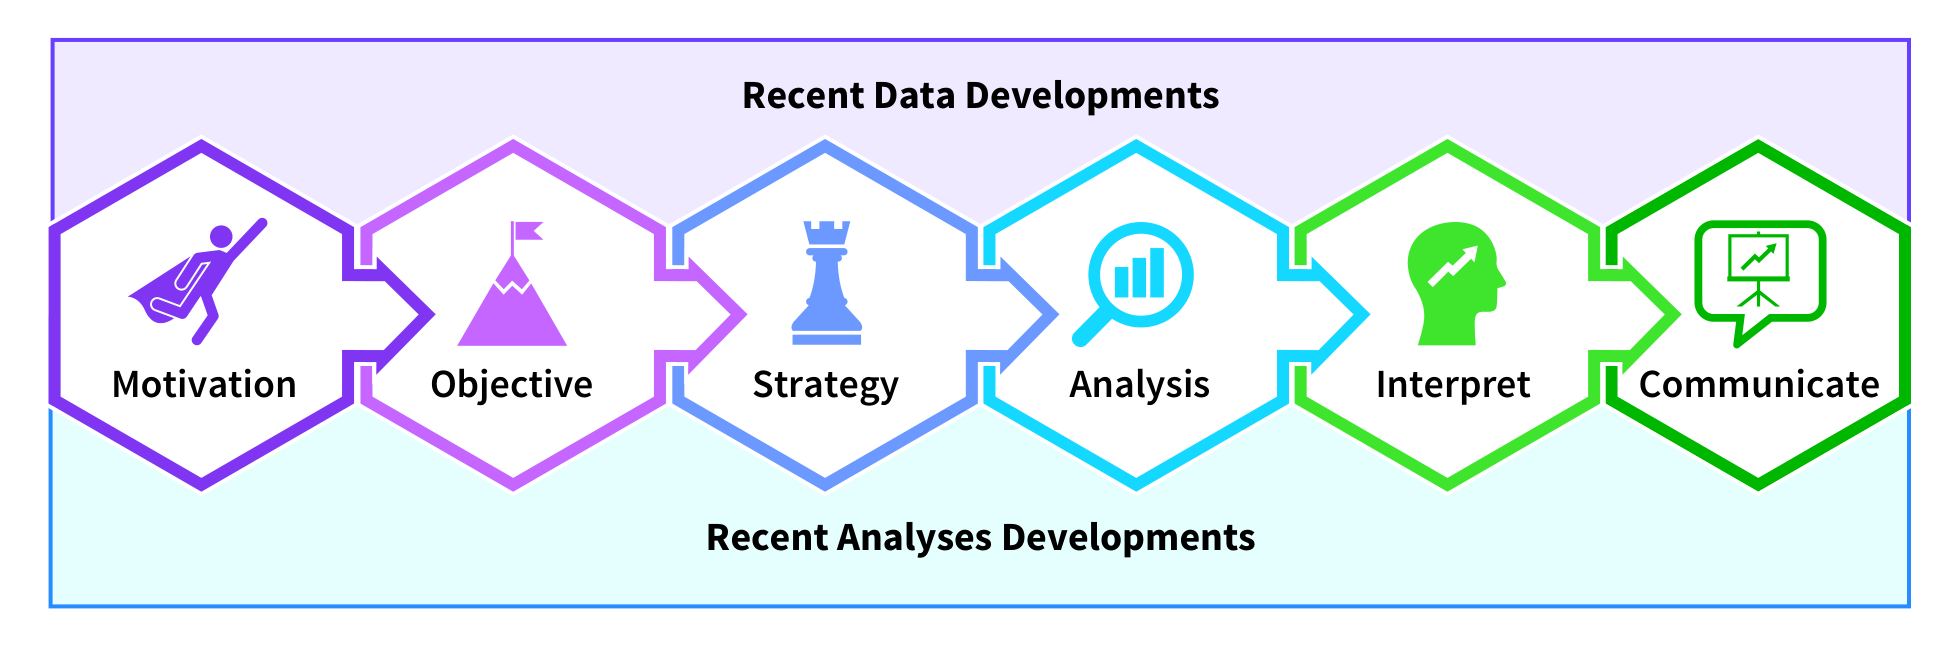
\includegraphics[width=0.95\textwidth,height=0.75\textheight,keepaspectratio]{../textbookForPractice/Figures/Ch_10/Intro 10.0.png}
    \end{figure}
\end{frame}

\begin{frame}{ILLUSTRATION 10.1}

    \begin{figure}[h]
        \centering
        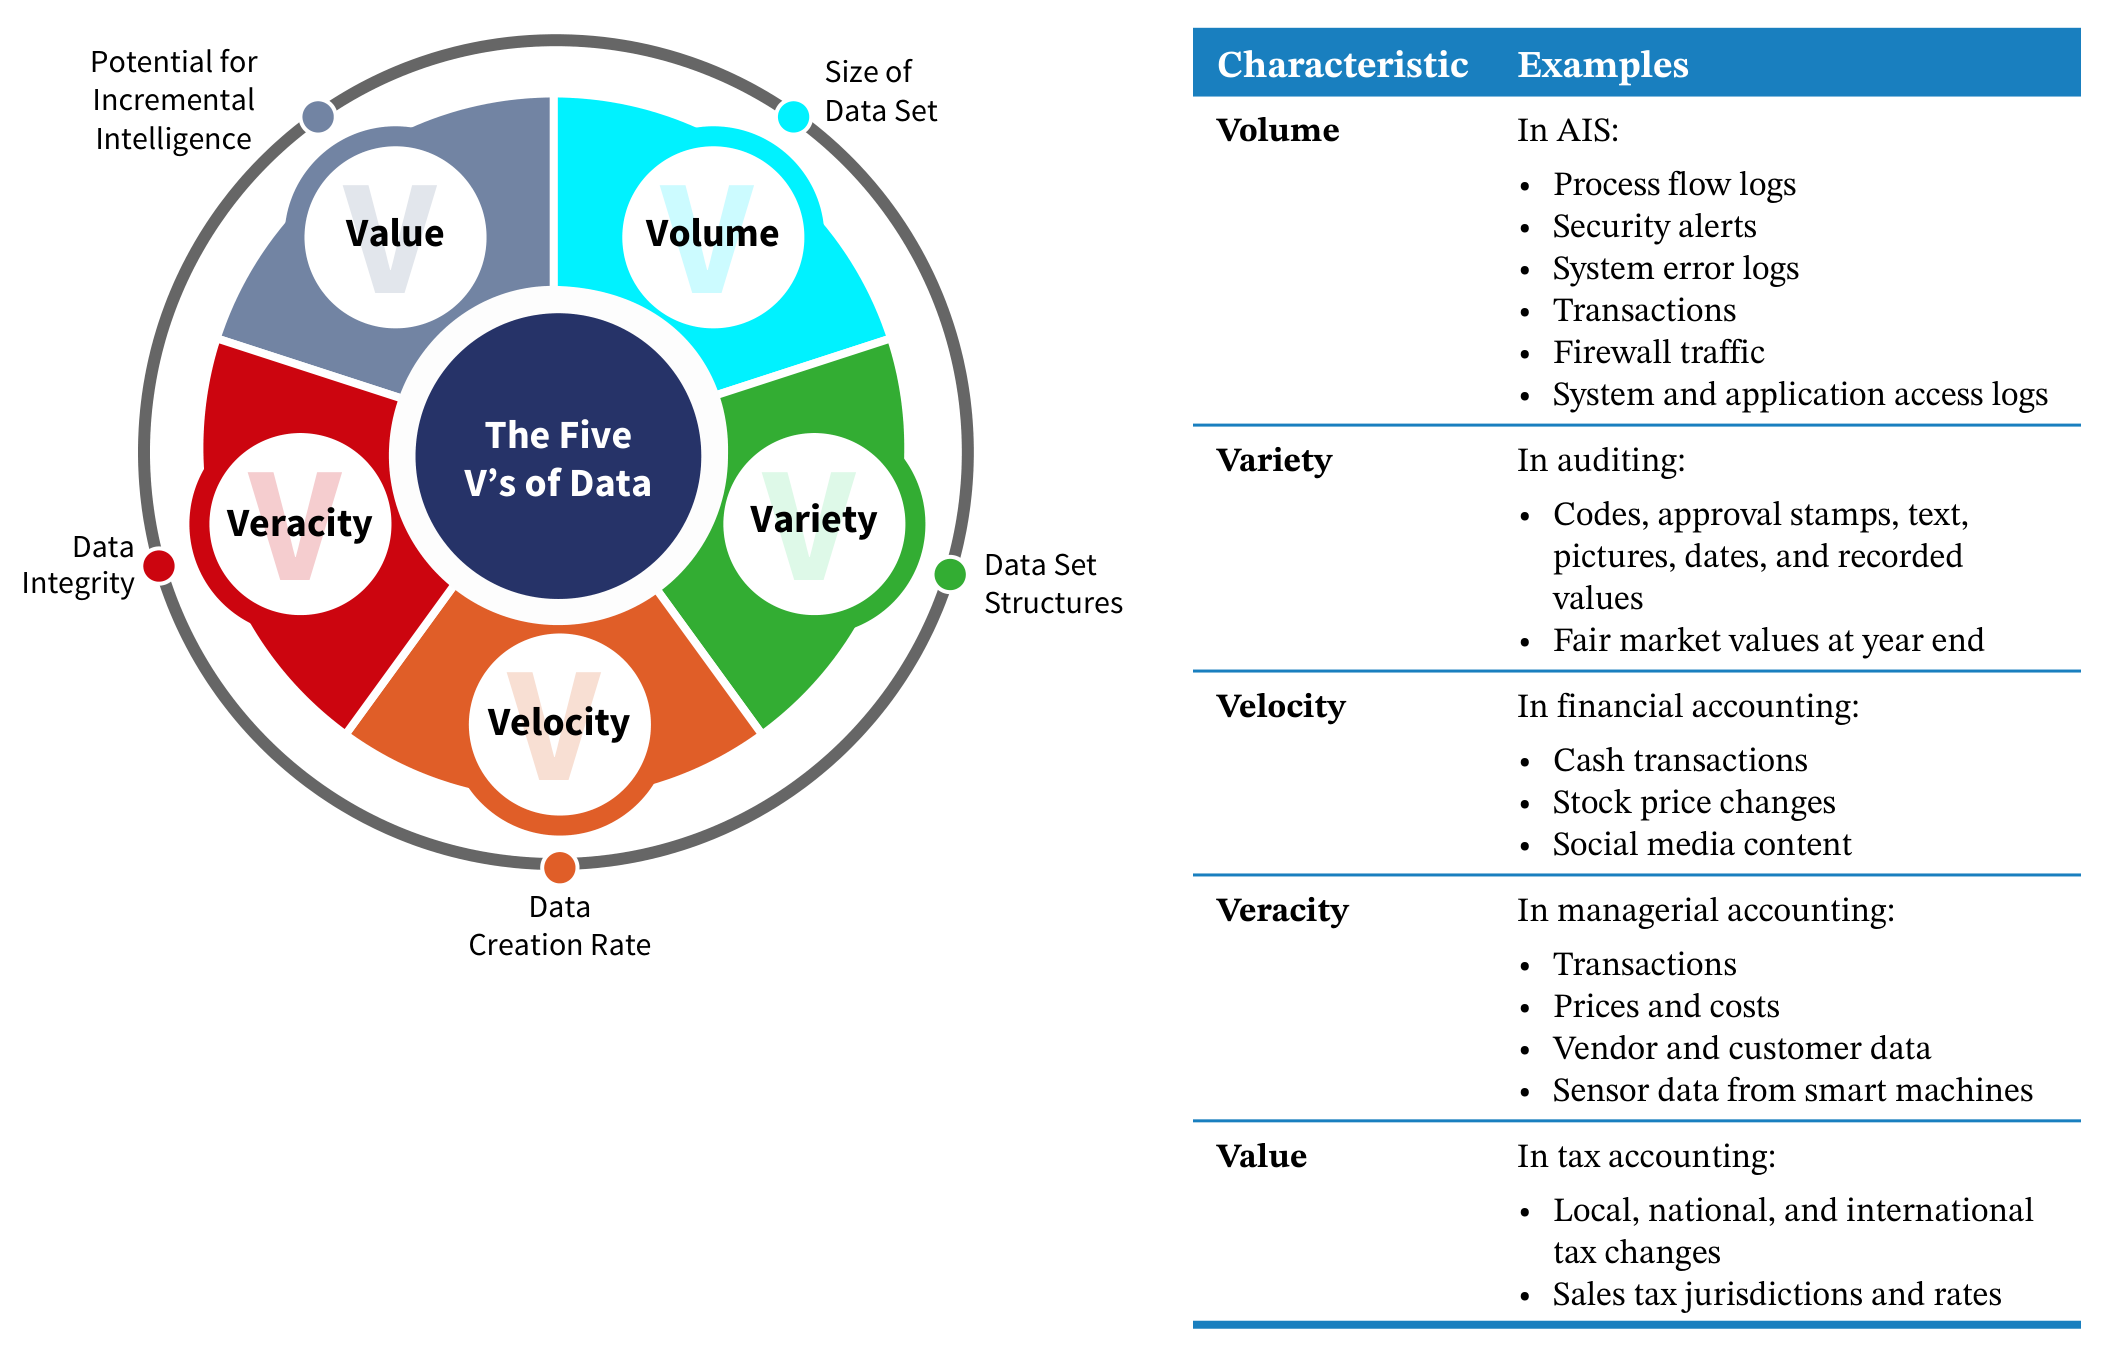
\includegraphics[width=0.95\textwidth,height=0.75\textheight,keepaspectratio]{../textbookForPractice/Figures/Ch_10/ILLUSTRATION 10.1.png}
    \end{figure}
\end{frame}

\begin{frame}{ILLUSTRATION 10.2}

    \begin{figure}[h]
        \centering
        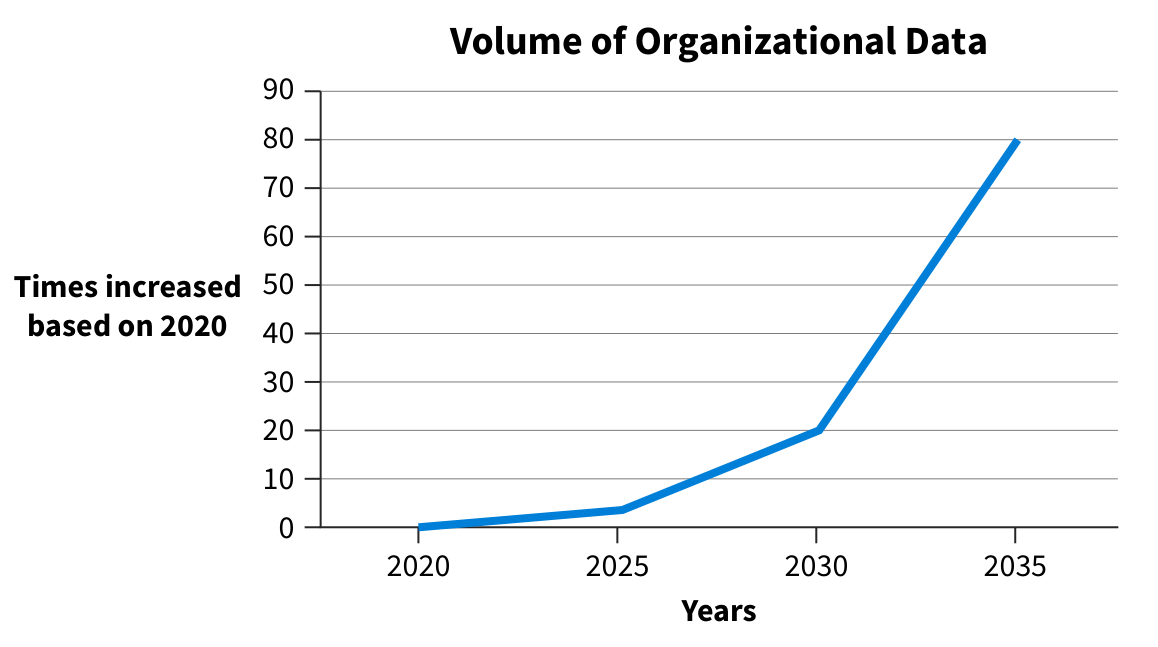
\includegraphics[width=0.95\textwidth,height=0.75\textheight,keepaspectratio]{../textbookForPractice/Figures/Ch_10/ILLUSTRATION 10.2.png}
    \end{figure}
\end{frame}

\begin{frame}{Chương 10: Các Xu hướng Dữ liệu và Phân tích Mới nhất}
\begin{itemize}
    \item \textbf{Mục tiêu:} Khám phá tác động của công nghệ và phân tích dữ liệu tiên tiến đối với nghề kế toán.
    \item \textbf{Trọng tâm:} Hiểu các đặc tính của Big Data và sự chuyển dịch của các công nghệ lõi.
    \item \textbf{Cấu trúc:} Dữ liệu lớn (Big Data), Sự phát triển của công nghệ, Ứng dụng vào các lĩnh vực kế toán.
\end{itemize}
\end{frame}

\begin{frame}{ILLUSTRATION 10.3}

    \begin{figure}[h]
        \centering
        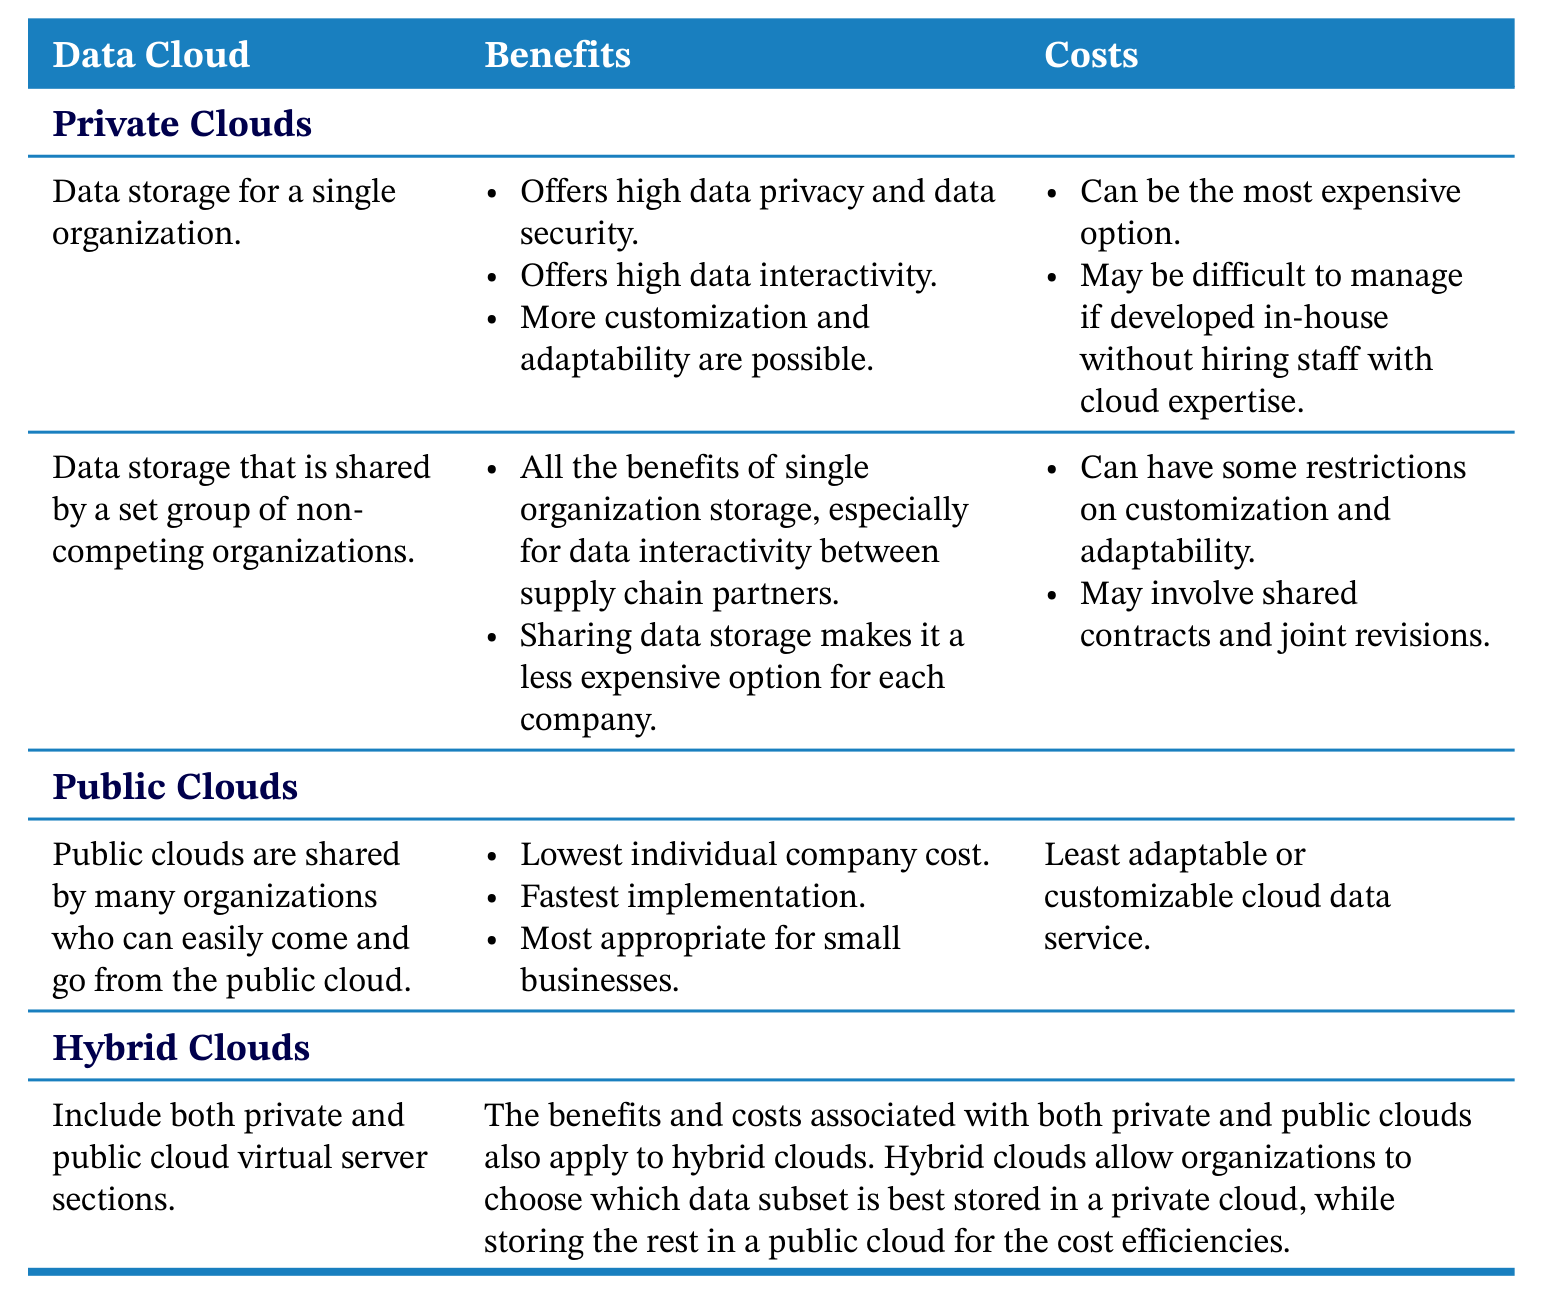
\includegraphics[width=0.95\textwidth,height=0.75\textheight,keepaspectratio]{../textbookForPractice/Figures/Ch_10/ILLUSTRATION 10.3.png}
    \end{figure}
\end{frame}

\begin{frame}{ILLUSTRATION 10.4}

    \begin{figure}[h]
        \centering
        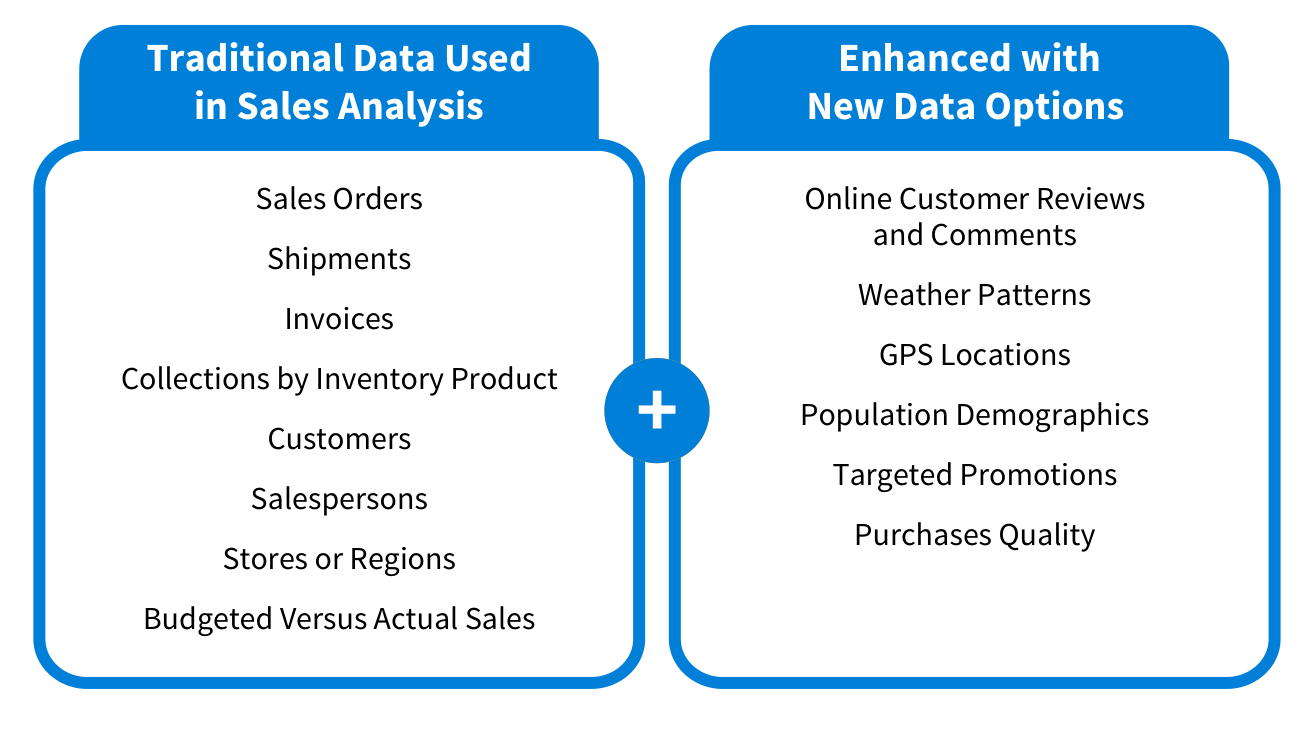
\includegraphics[width=0.95\textwidth,height=0.75\textheight,keepaspectratio]{../textbookForPractice/Figures/Ch_10/ILLUSTRATION 10.4.png}
    \end{figure}
\end{frame}

\begin{frame}{10.1 Đặc điểm của Dữ liệu lớn (5V của Big Data)}
\begin{itemize}
    \item Sự bùng nổ dữ liệu yêu cầu thay đổi trong phương pháp phân tích.
    \item Mô hình 5V giải thích bản chất đa chiều của Dữ liệu lớn:
    \begin{itemize}
        \item Volume (Khối lượng)
        \item Variety (Đa dạng)
        \item Velocity (Tốc độ)
        \item Veracity (Tính xác thực)
        \item Value (Giá trị)
    \end{itemize}
\end{itemize}
\end{frame}

\begin{frame}{ILLUSTRATION 10.5}

    \begin{figure}[h]
        \centering
        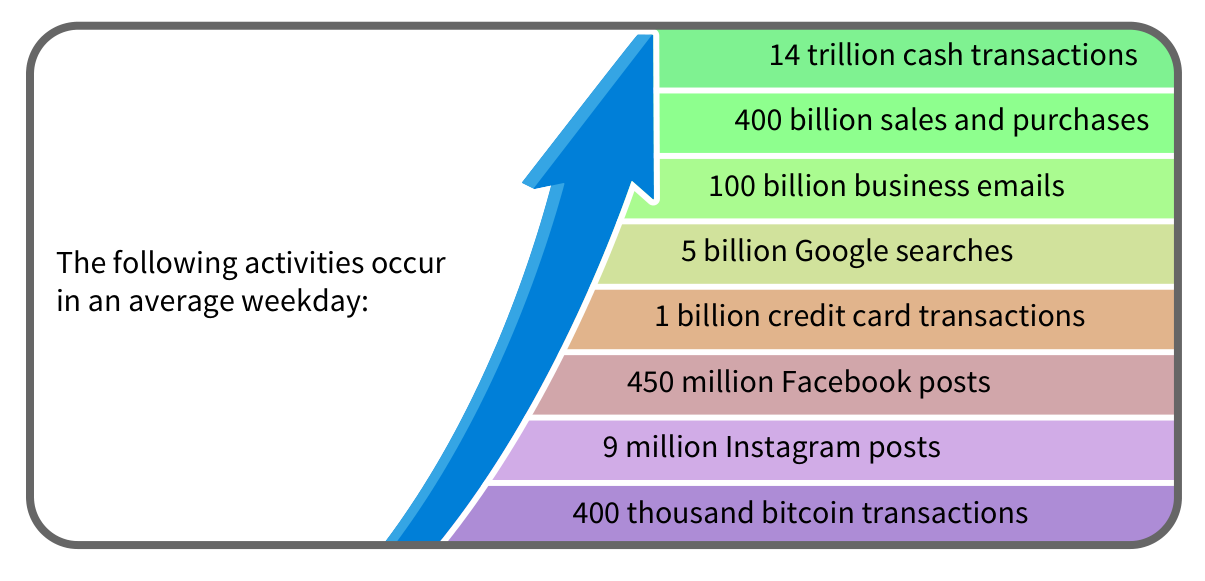
\includegraphics[width=0.95\textwidth,height=0.75\textheight,keepaspectratio]{../textbookForPractice/Figures/Ch_10/ILLUSTRATION 10.5.png}
    \end{figure}
\end{frame}

\begin{frame}{ILLUSTRATION 10.6}

    \begin{figure}[h]
        \centering
        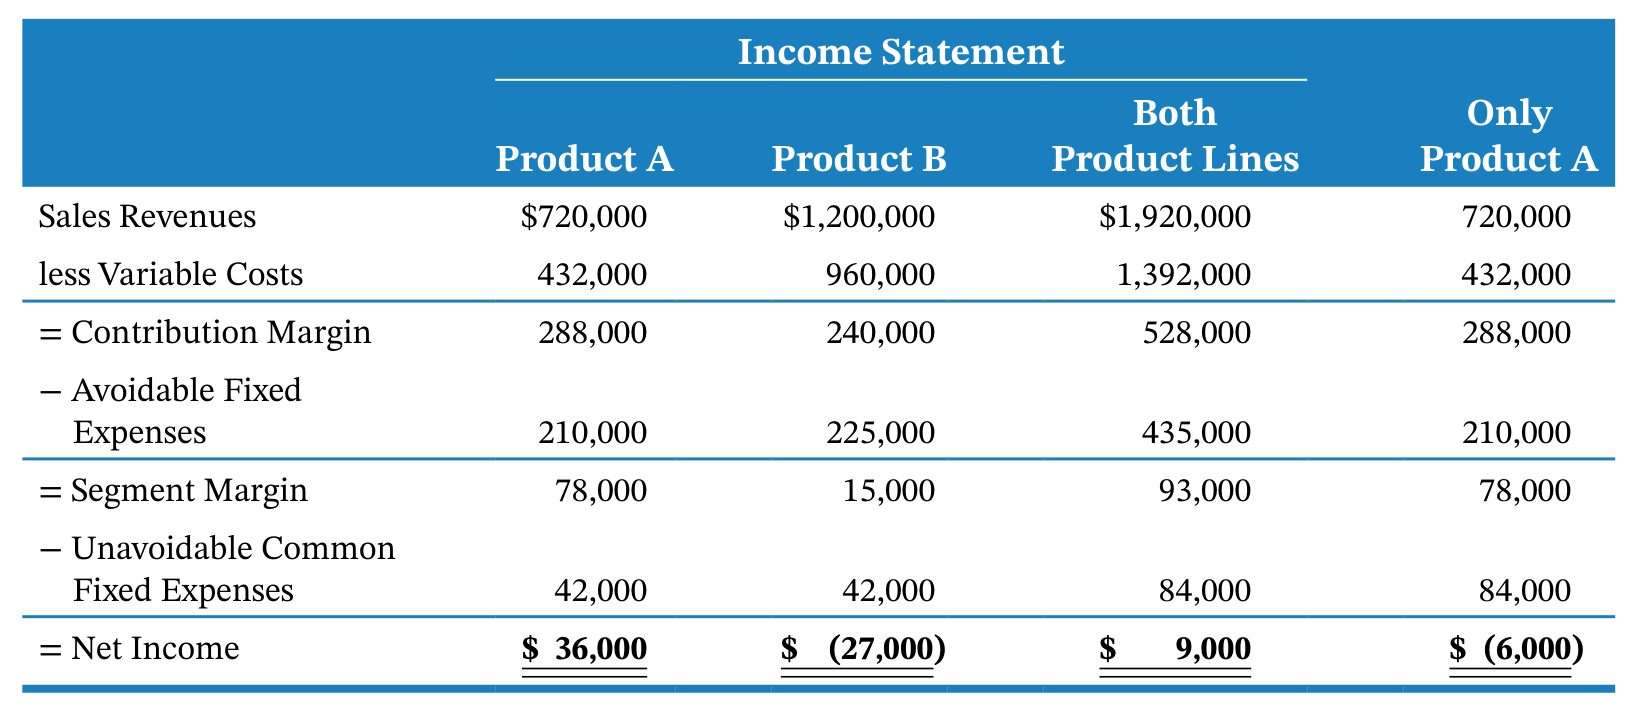
\includegraphics[width=0.95\textwidth,height=0.75\textheight,keepaspectratio]{../textbookForPractice/Figures/Ch_10/ILLUSTRATION 10.6.png}
    \end{figure}
\end{frame}

\begin{frame}{Volume (Khối lượng) \& Variety (Đa dạng)}
\begin{itemize}
    \item \textbf{Volume:} Lượng dữ liệu vượt ra khỏi khả năng xử lý của Excel hoặc SQL thông thường. Được tính bằng Terabyte, Petabyte,...
    \item \textbf{Variety:}
    \begin{itemize}
        \item Dữ liệu có cấu trúc (Bảng tính, CSDL)
        \item Dữ liệu bán cấu trúc (XML, JSON, XBRL)
        \item Dữ liệu phi cấu trúc (Văn bản, Hình ảnh, Âm thanh) chiếm đến 80\% tổng lượng dữ liệu hiện nay.
    \end{itemize}
\end{itemize}
\end{frame}

\begin{frame}{ILLUSTRATION 10.7}

    \begin{figure}[h]
        \centering
        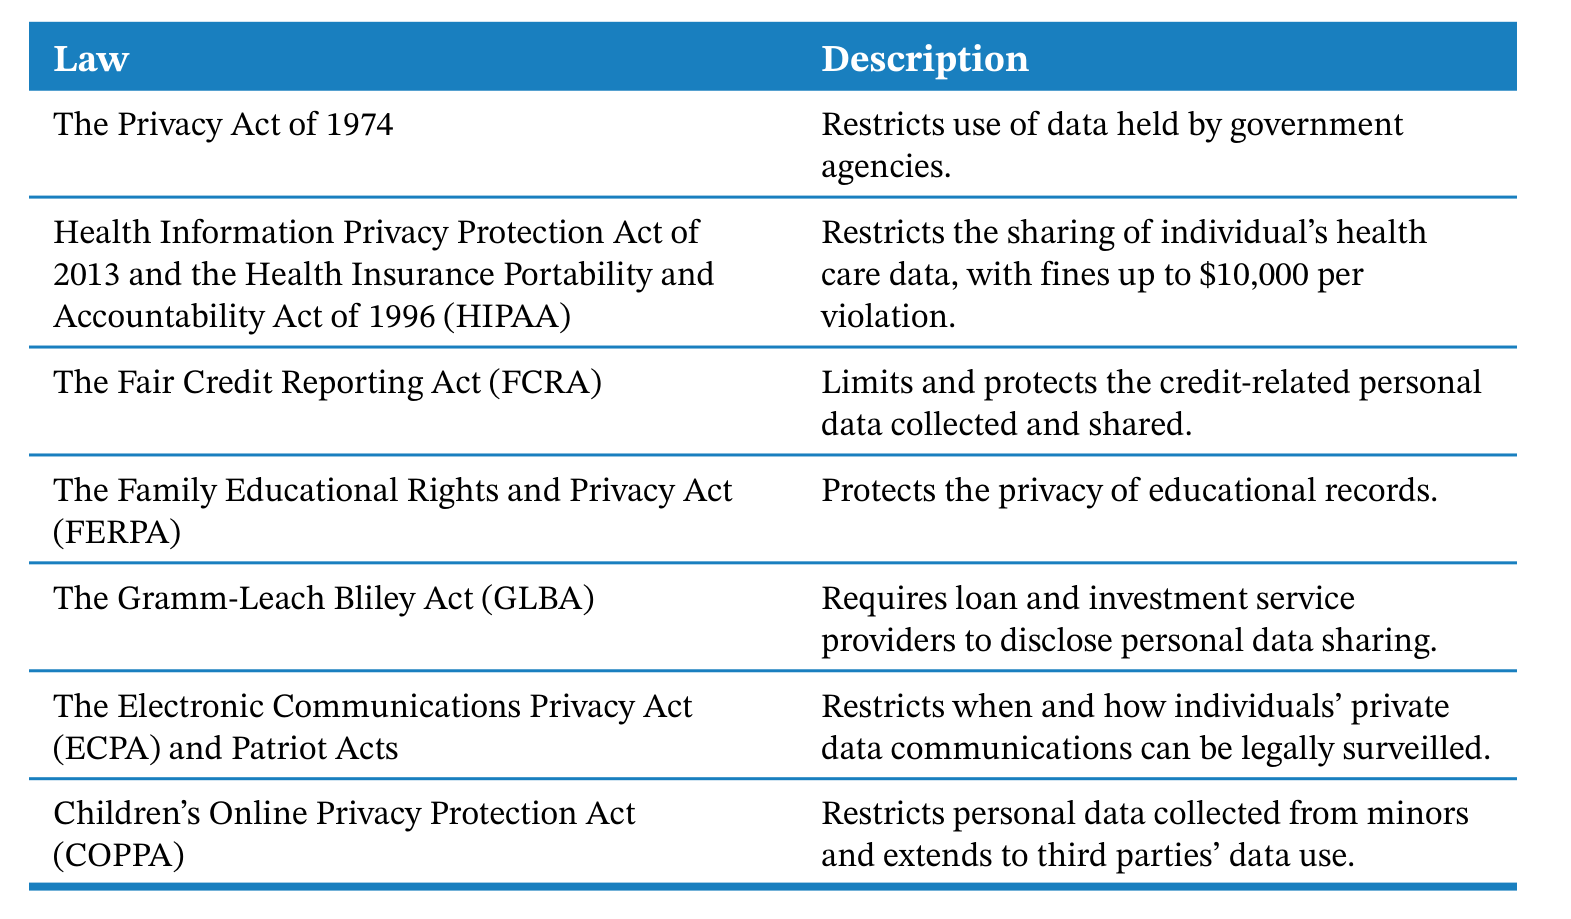
\includegraphics[width=0.95\textwidth,height=0.75\textheight,keepaspectratio]{../textbookForPractice/Figures/Ch_10/ILLUSTRATION 10.7.png}
    \end{figure}
\end{frame}

\begin{frame}{ILLUSTRATION 10.8}

    \begin{figure}[h]
        \centering
        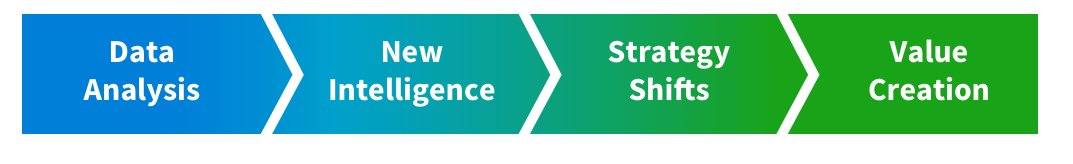
\includegraphics[width=0.95\textwidth,height=0.75\textheight,keepaspectratio]{../textbookForPractice/Figures/Ch_10/ILLUSTRATION 10.8.png}
    \end{figure}
\end{frame}

\begin{frame}{Velocity (Tốc độ) \& Veracity (Tính xác thực)}
\begin{itemize}
    \item \textbf{Velocity:} Tốc độ sinh ra và luân chuyển của dữ liệu. Doanh nghiệp cần xử lý dữ liệu theo thời gian thực (Real-time).
    \item \textbf{Veracity:} Mức độ đáng tin cậy. Dữ liệu từ mạng xã hội có thể bị nhiễu và sai lệch (bias), dẫn đến rủi ro ra quyết định sai lầm.
\end{itemize}
\end{frame}

\begin{frame}{ILLUSTRATION 10.9}

    \begin{figure}[h]
        \centering
        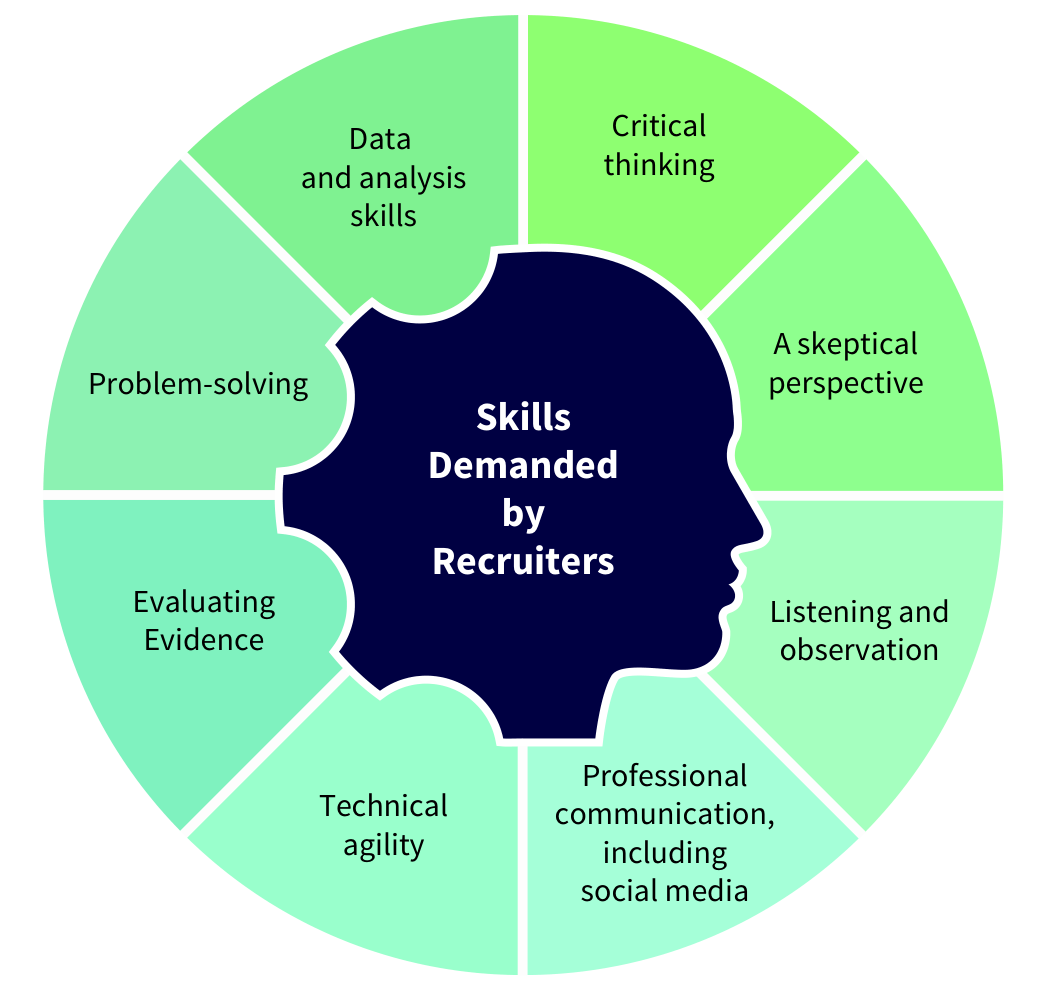
\includegraphics[width=0.95\textwidth,height=0.75\textheight,keepaspectratio]{../textbookForPractice/Figures/Ch_10/ILLUSTRATION 10.9.png}
    \end{figure}
\end{frame}

\begin{frame}{ILLUSTRATION 10.10}

    \begin{figure}[h]
        \centering
        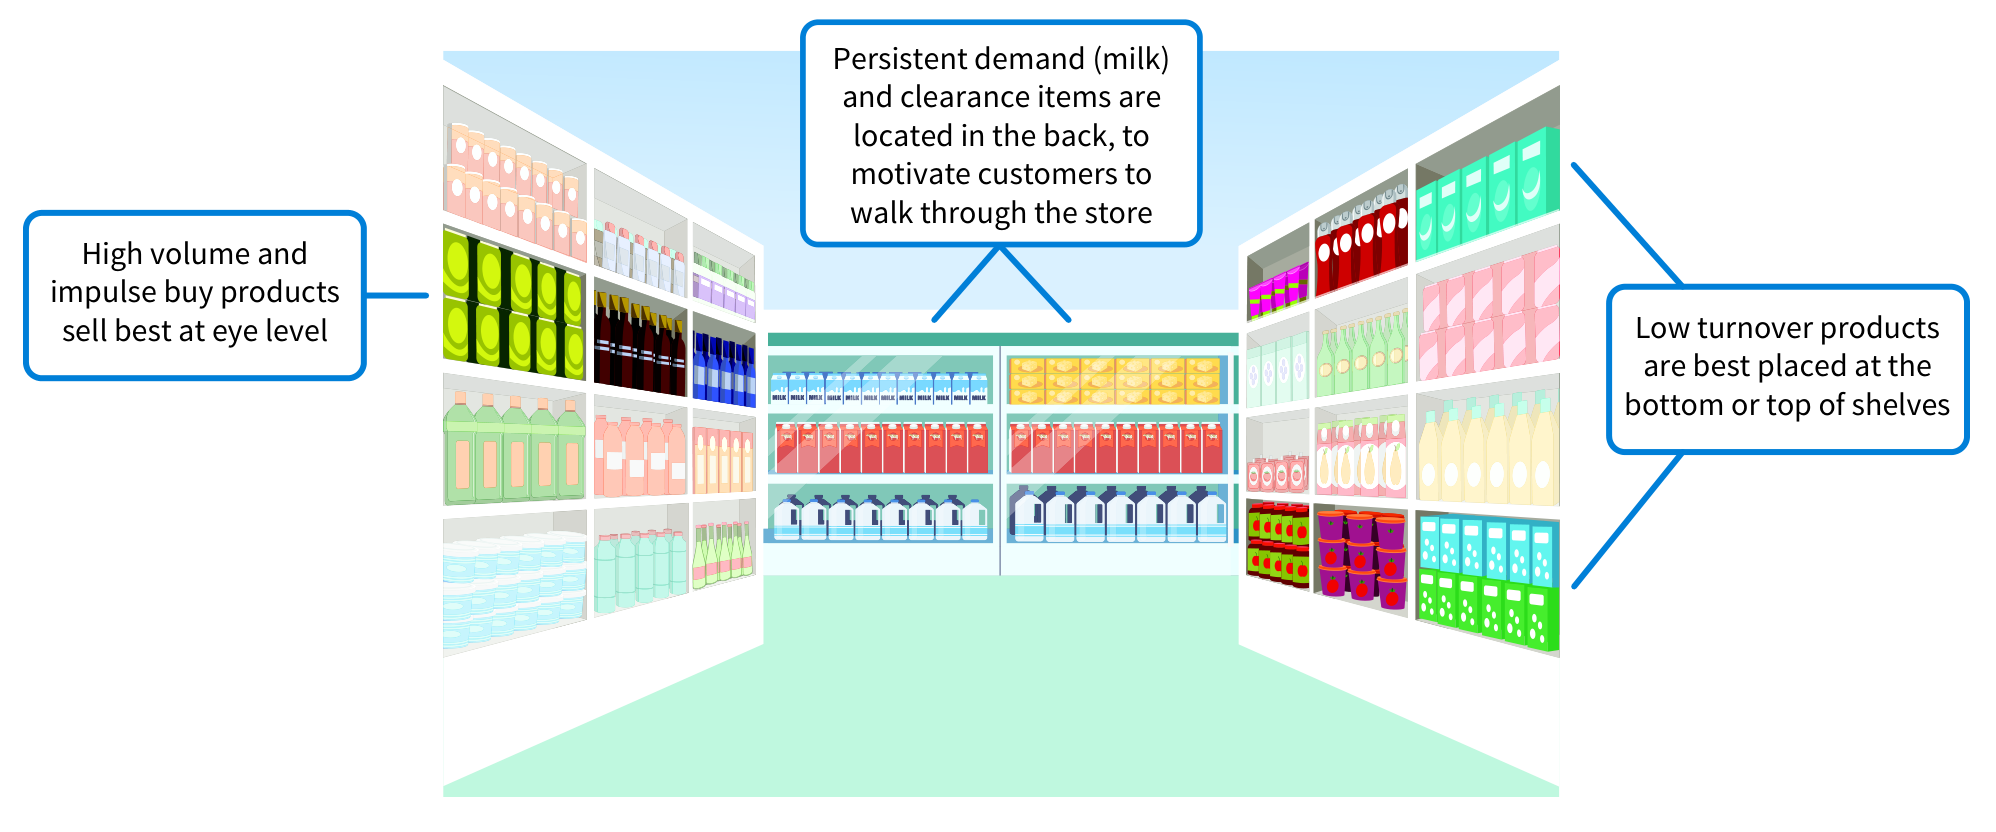
\includegraphics[width=0.95\textwidth,height=0.75\textheight,keepaspectratio]{../textbookForPractice/Figures/Ch_10/ILLUSTRATION 10.10.png}
    \end{figure}
\end{frame}

\begin{frame}{Value (Giá trị)}
\begin{itemize}
    \item \textbf{Value:} Tất cả 4V trước đều vô nghĩa nếu không thể trích xuất ra insight có giá trị (Value) cho doanh nghiệp.
    \item Đối với kế toán, Value thể hiện ở khả năng:
    \begin{itemize}
        \item Dự báo dòng tiền chính xác hơn.
        \item Nhận diện gian lận nhanh hơn.
        \item Tiết kiệm chi phí vận hành.
    \end{itemize}
\end{itemize}
\end{frame}

\begin{frame}{ILLUSTRATION 10.11}

    \begin{figure}[h]
        \centering
        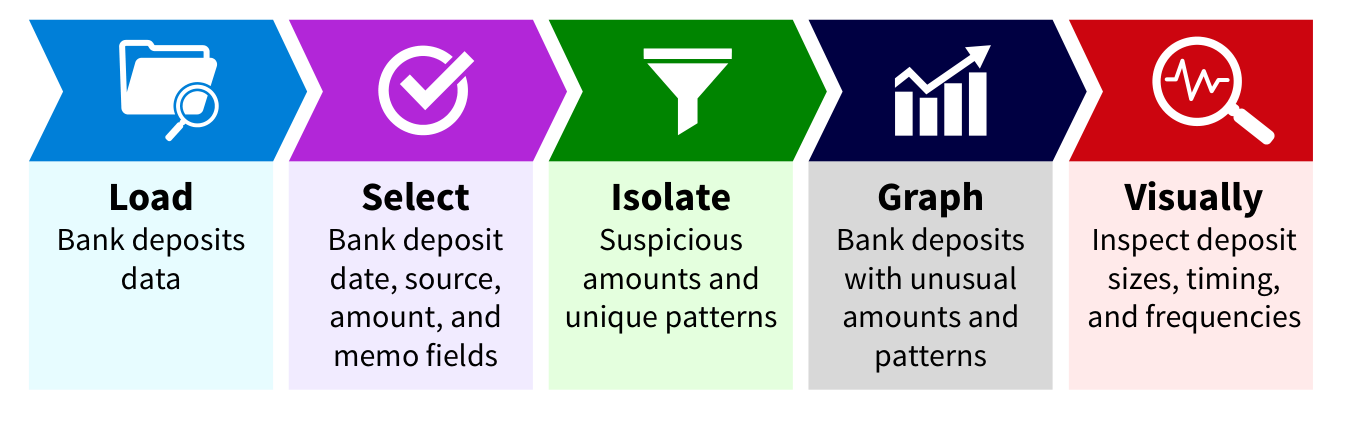
\includegraphics[width=0.95\textwidth,height=0.75\textheight,keepaspectratio]{../textbookForPractice/Figures/Ch_10/ILLUSTRATION 10.11.png}
    \end{figure}
\end{frame}

\begin{frame}{ILLUSTRATION 10.12}

    \begin{figure}[h]
        \centering
        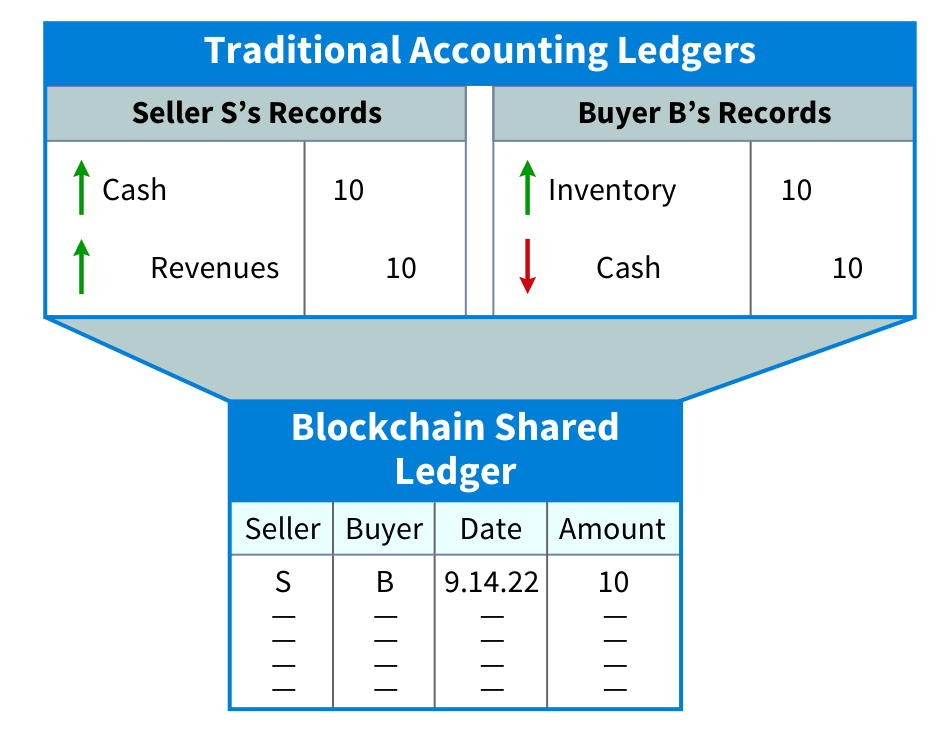
\includegraphics[width=0.95\textwidth,height=0.75\textheight,keepaspectratio]{../textbookForPractice/Figures/Ch_10/ILLUSTRATION 10.12.png}
    \end{figure}
\end{frame}

\begin{frame}{Đạo đức Dữ liệu (Data Ethics)}
\begin{itemize}
    \item \textbf{Quyền riêng tư (Privacy):} Bảo mật thông tin nhận dạng cá nhân (PII) trong quá trình phân tích.
    \item \textbf{Tính minh bạch (Transparency):} Người dùng cần biết thuật toán AI đưa ra quyết định dựa trên điều gì.
    \item \textbf{Thiên lệch (Bias):} Dữ liệu lịch sử mang định kiến sẽ dạy cho AI đưa ra những quyết định phân biệt đối xử.
\end{itemize}
\end{frame}

\begin{frame}{ILLUSTRATION 10.13}

    \begin{figure}[h]
        \centering
        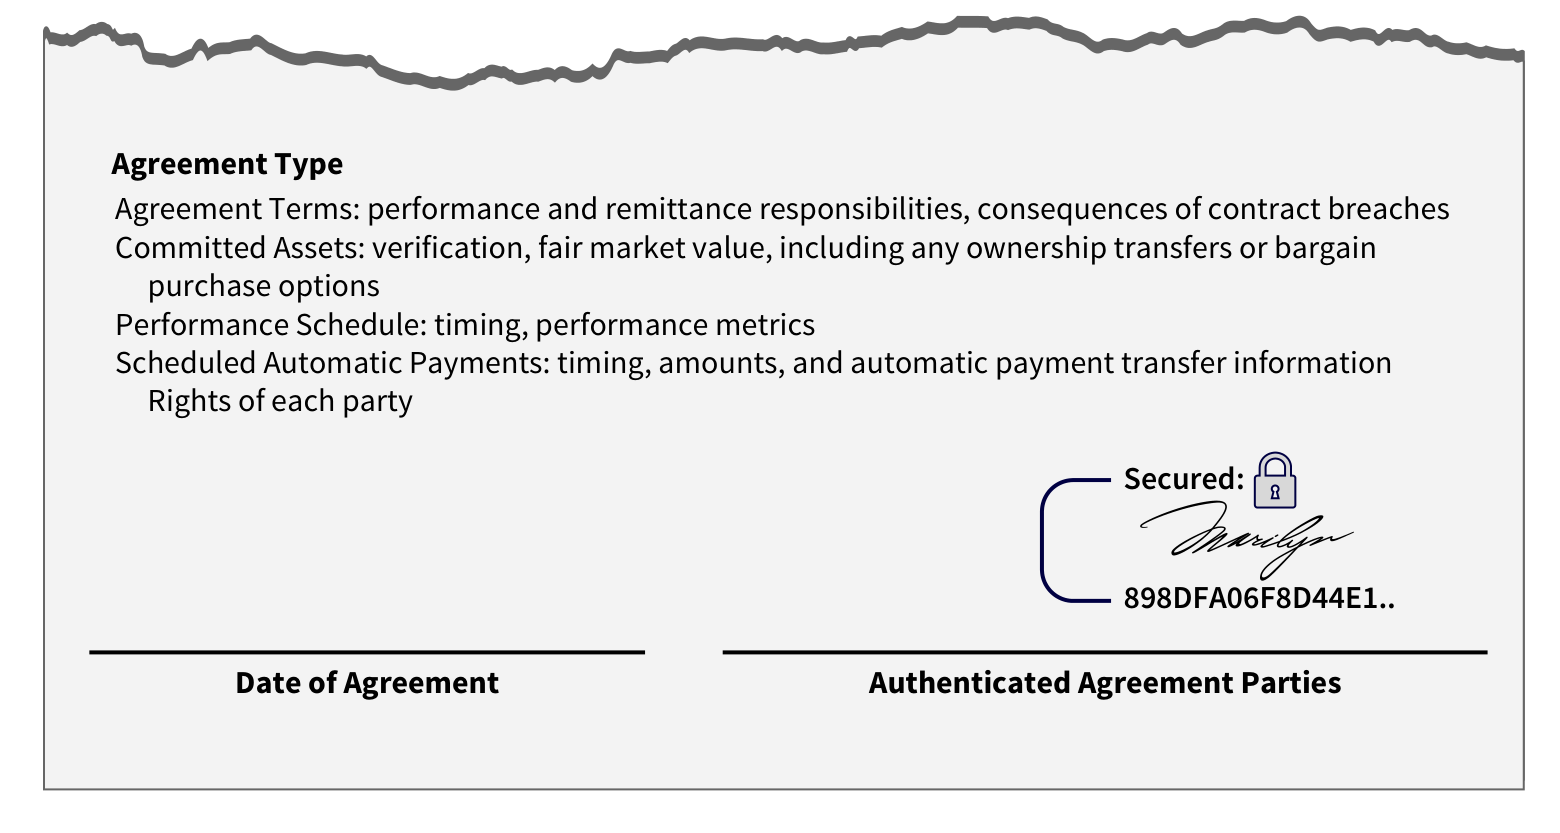
\includegraphics[width=0.95\textwidth,height=0.75\textheight,keepaspectratio]{../textbookForPractice/Figures/Ch_10/ILLUSTRATION 10.13.png}
    \end{figure}
\end{frame}

\begin{frame}{ILLUSTRATION 10.14}

    \begin{figure}[h]
        \centering
        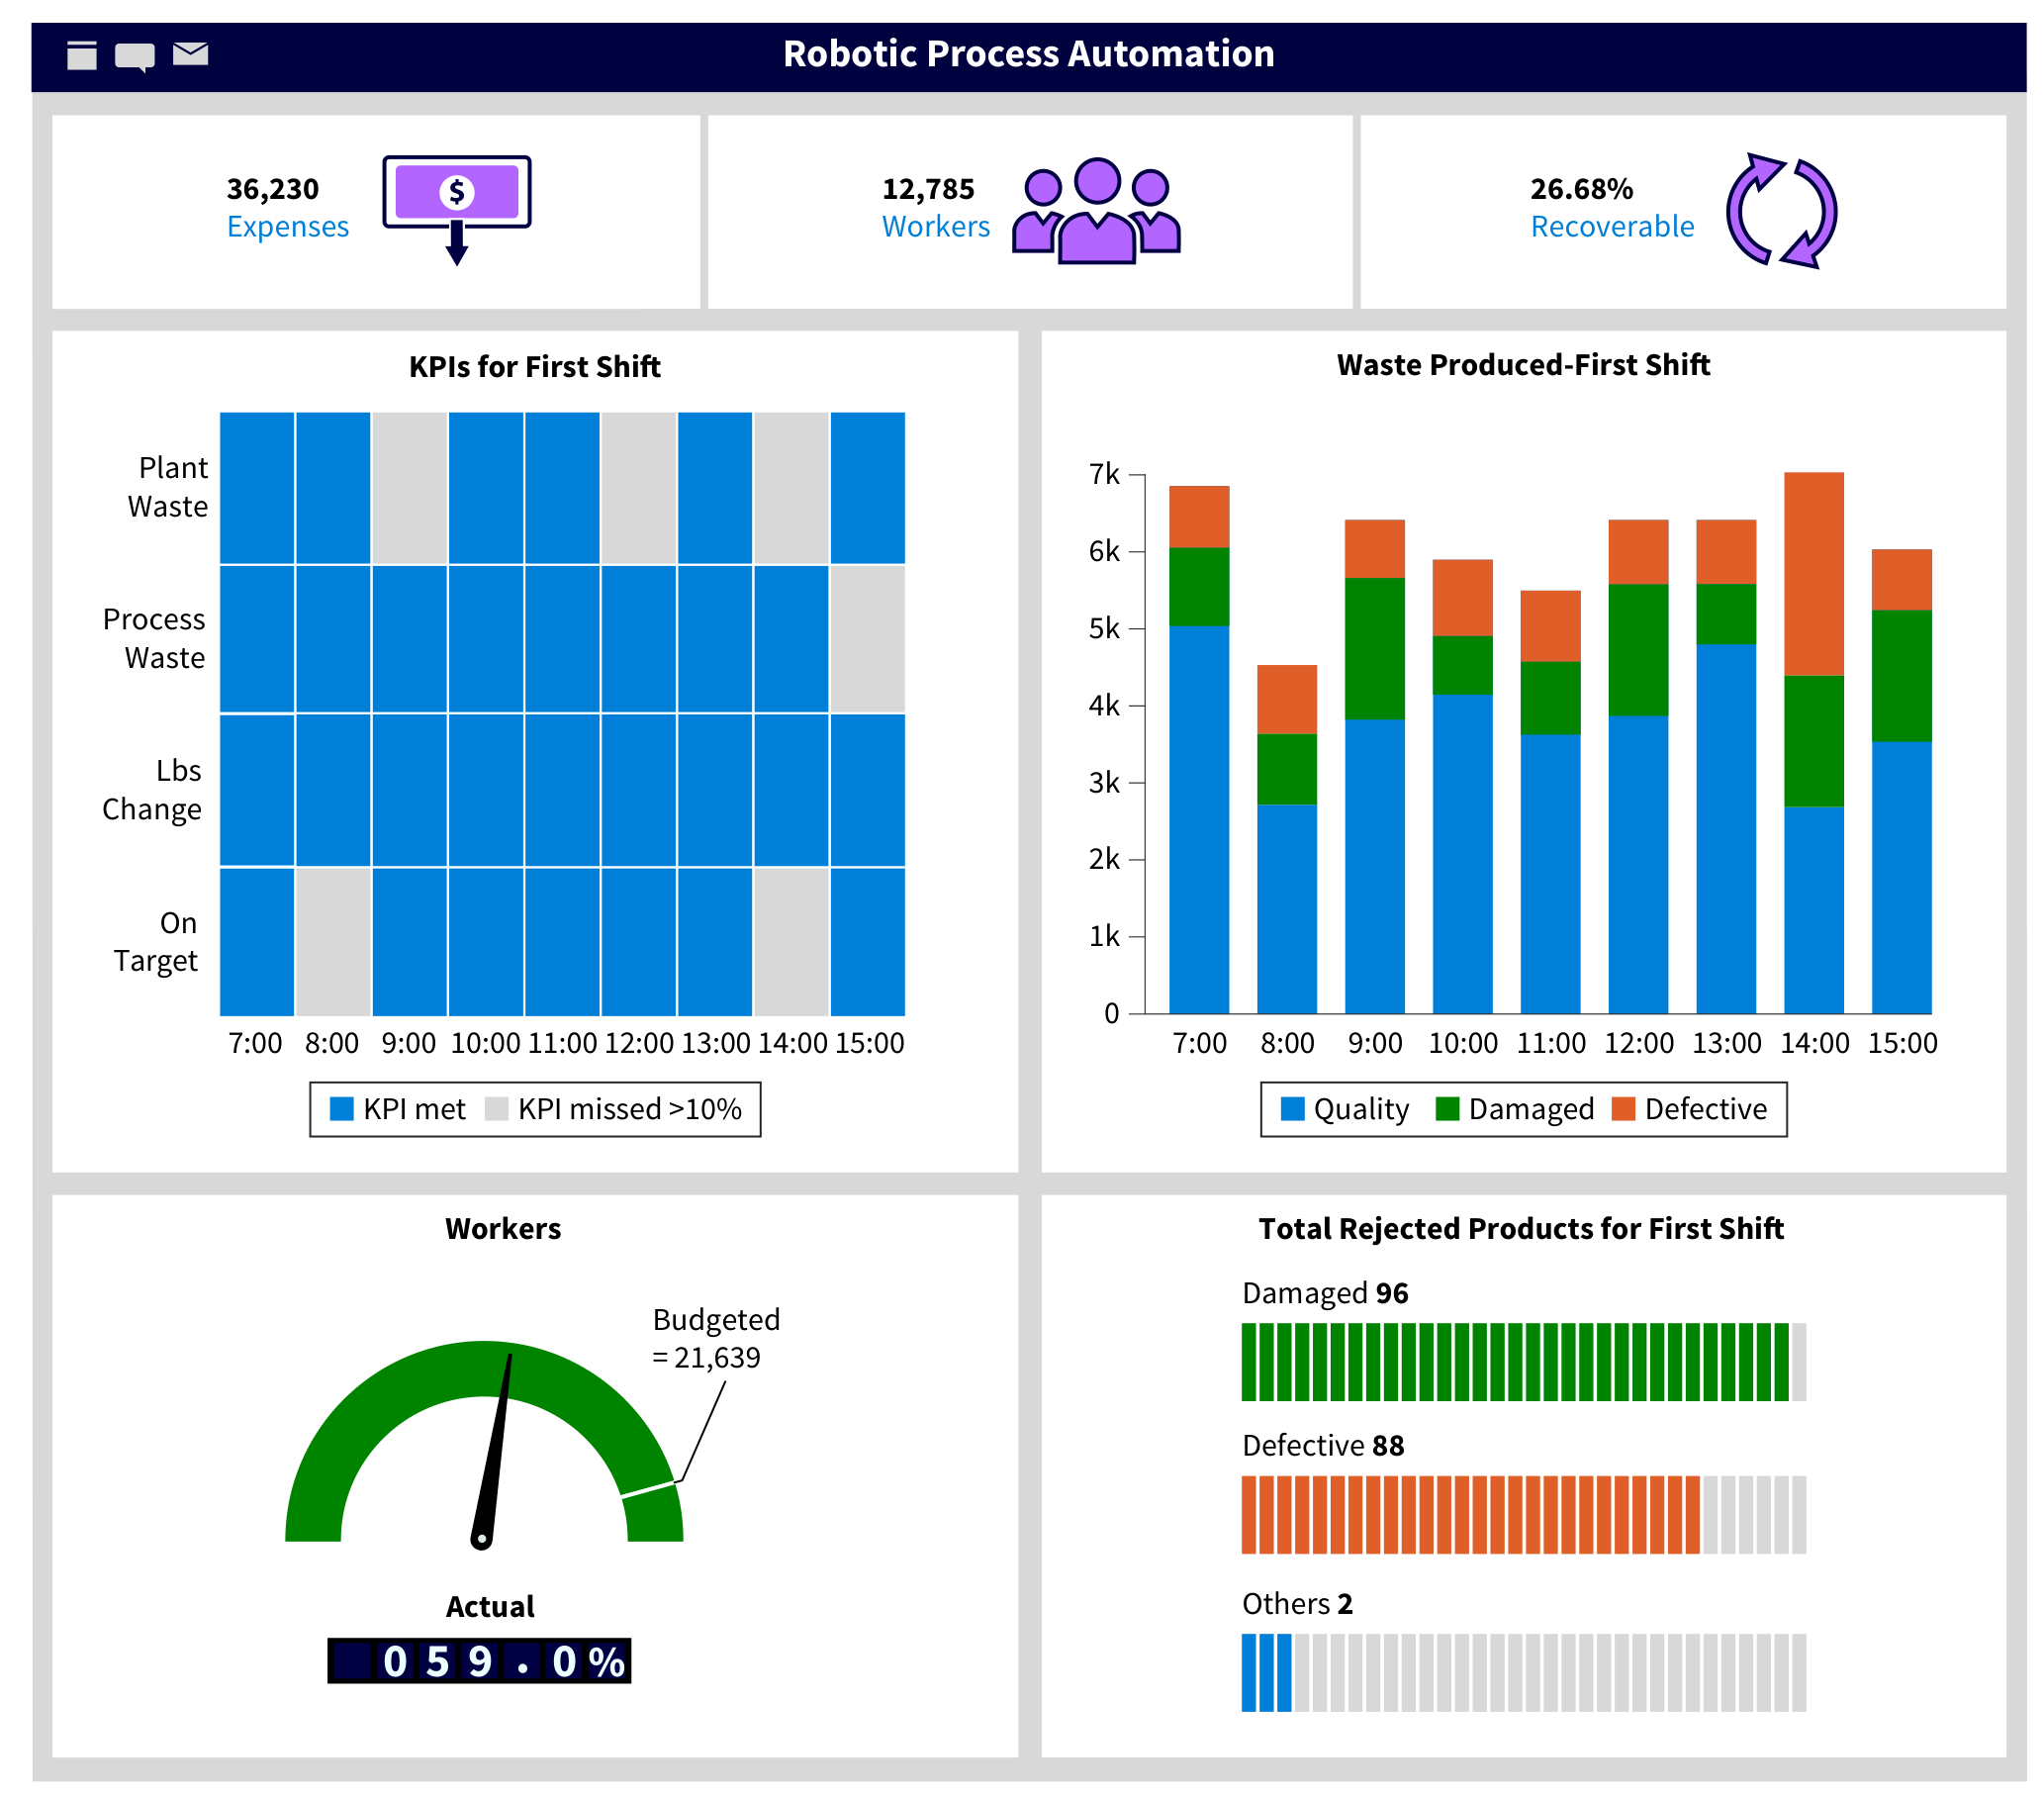
\includegraphics[width=0.95\textwidth,height=0.75\textheight,keepaspectratio]{../textbookForPractice/Figures/Ch_10/ILLUSTRATION 10.14.png}
    \end{figure}
\end{frame}

\begin{frame}{10.2 Công Nghệ Thay Đổi Phân Tích Dữ Liệu}
\begin{itemize}
    \item \textbf{Value Creation (Mục tiêu tạo giá trị):} Công nghệ không chỉ để lưu trữ mà phải tự động hóa, phân tích sâu và cung cấp dự đoán.
    \item Sự hội tụ của Cloud Computing, AI và Blockchain đang tái định hình cách bộ phận Kế toán làm việc hàng ngày.
\end{itemize}
\end{frame}

\begin{frame}{ILLUSTRATION 10.15}

    \begin{figure}[h]
        \centering
        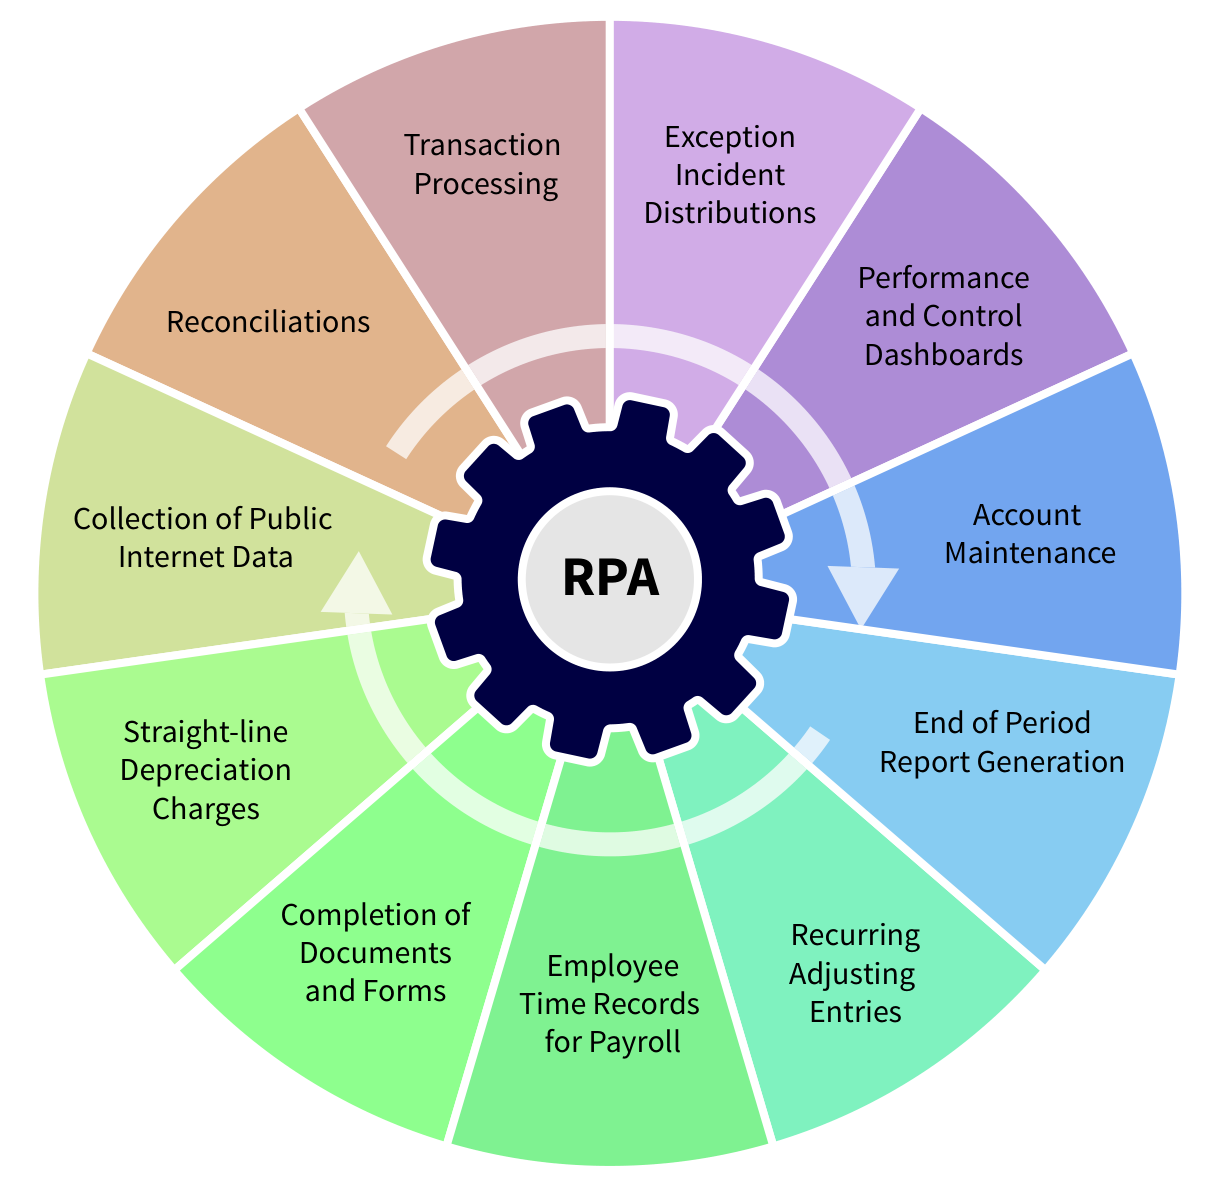
\includegraphics[width=0.95\textwidth,height=0.75\textheight,keepaspectratio]{../textbookForPractice/Figures/Ch_10/ILLUSTRATION 10.15.png}
    \end{figure}
\end{frame}

\begin{frame}{ILLUSTRATION 10.16}

    \begin{figure}[h]
        \centering
        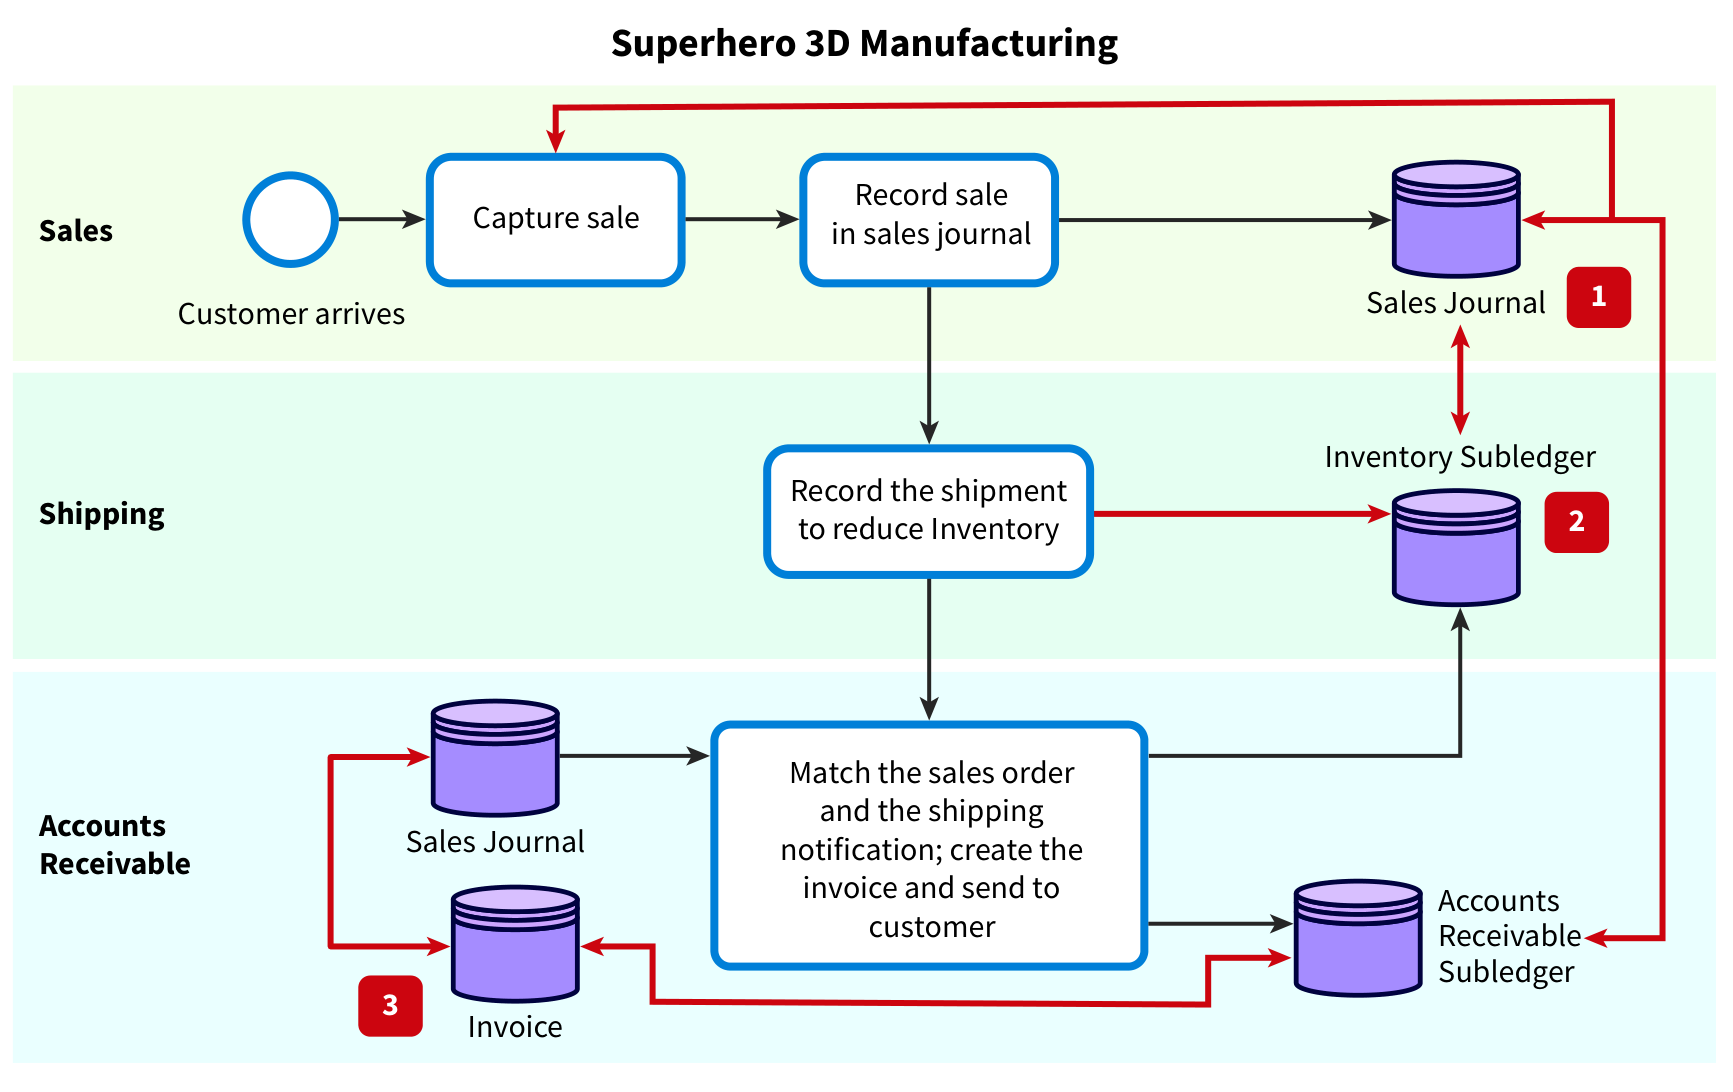
\includegraphics[width=0.95\textwidth,height=0.75\textheight,keepaspectratio]{../textbookForPractice/Figures/Ch_10/ILLUSTRATION 10.16.png}
    \end{figure}
\end{frame}

\begin{frame}{Khai phá Dữ liệu \& Hợp đồng Thông minh}
\begin{itemize}
    \item \textbf{Khai phá Dữ liệu (Data Mining):} Ứng dụng thống kê và học máy để tìm kiếm mô hình (pattern) ẩn trong cơ sở dữ liệu lớn.
    \item \textbf{Hợp đồng Thông minh (Smart Contracts):} Code chạy trên blockchain tự động thực thi các điều khoản hợp đồng khi điều kiện được thỏa mãn (VD: tự động thanh toán khi hàng được giao).
\end{itemize}
\end{frame}

\begin{frame}{ILLUSTRATION 10.17}

    \begin{figure}[h]
        \centering
        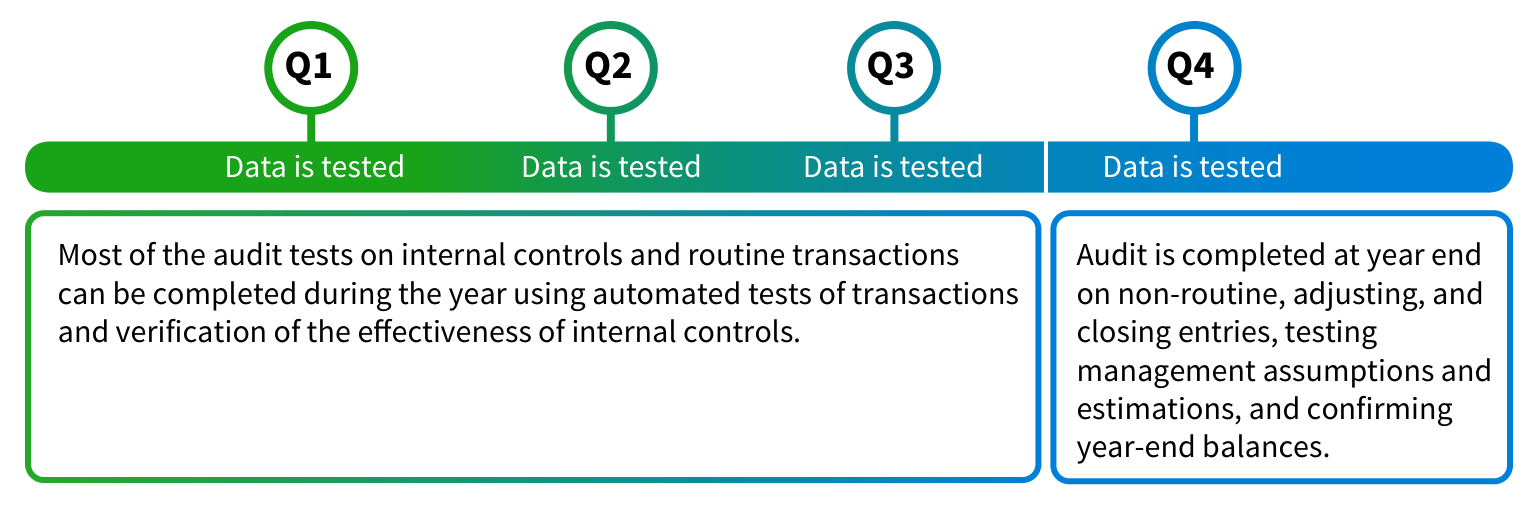
\includegraphics[width=0.95\textwidth,height=0.75\textheight,keepaspectratio]{../textbookForPractice/Figures/Ch_10/ILLUSTRATION 10.17.png}
    \end{figure}
\end{frame}

\begin{frame}{ILLUSTRATION 10.18}

    \begin{figure}[h]
        \centering
        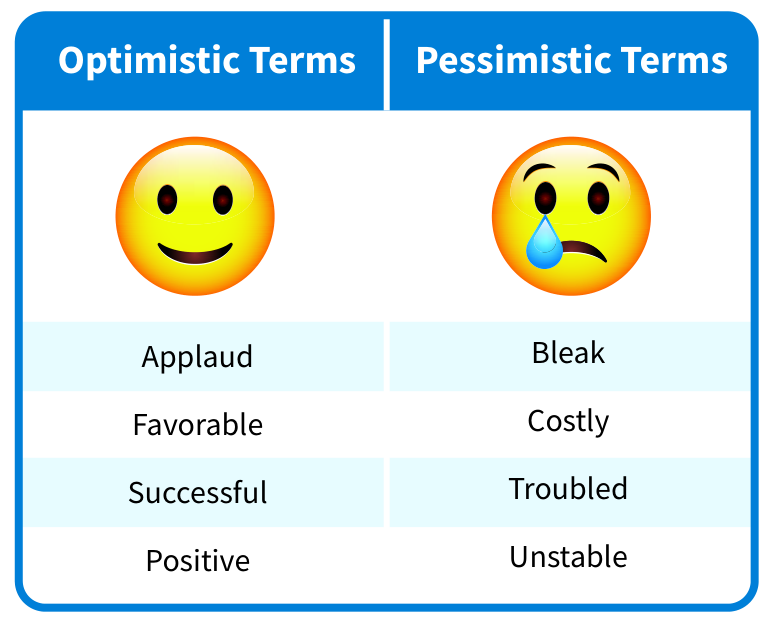
\includegraphics[width=0.95\textwidth,height=0.75\textheight,keepaspectratio]{../textbookForPractice/Figures/Ch_10/ILLUSTRATION 10.18.png}
    \end{figure}
\end{frame}

\begin{frame}{Tự Động Hóa Quy Trình Bằng Robot (RPA)}
\begin{itemize}
    \item \textbf{RPA (Robotic Process Automation):} Sử dụng phần mềm (bot) để tự động hóa các tác vụ lặp đi lặp lại có quy tắc cố định (VD: nhập liệu hóa đơn, đối chiếu ngân hàng).
    \item \textbf{Lợi ích:} Giảm thiểu lỗi sai (human error), giải phóng nhân sự kế toán cho công việc phân tích.
\end{itemize}
\end{frame}

\begin{frame}{ILLUSTRATION 10.19}

    \begin{figure}[h]
        \centering
        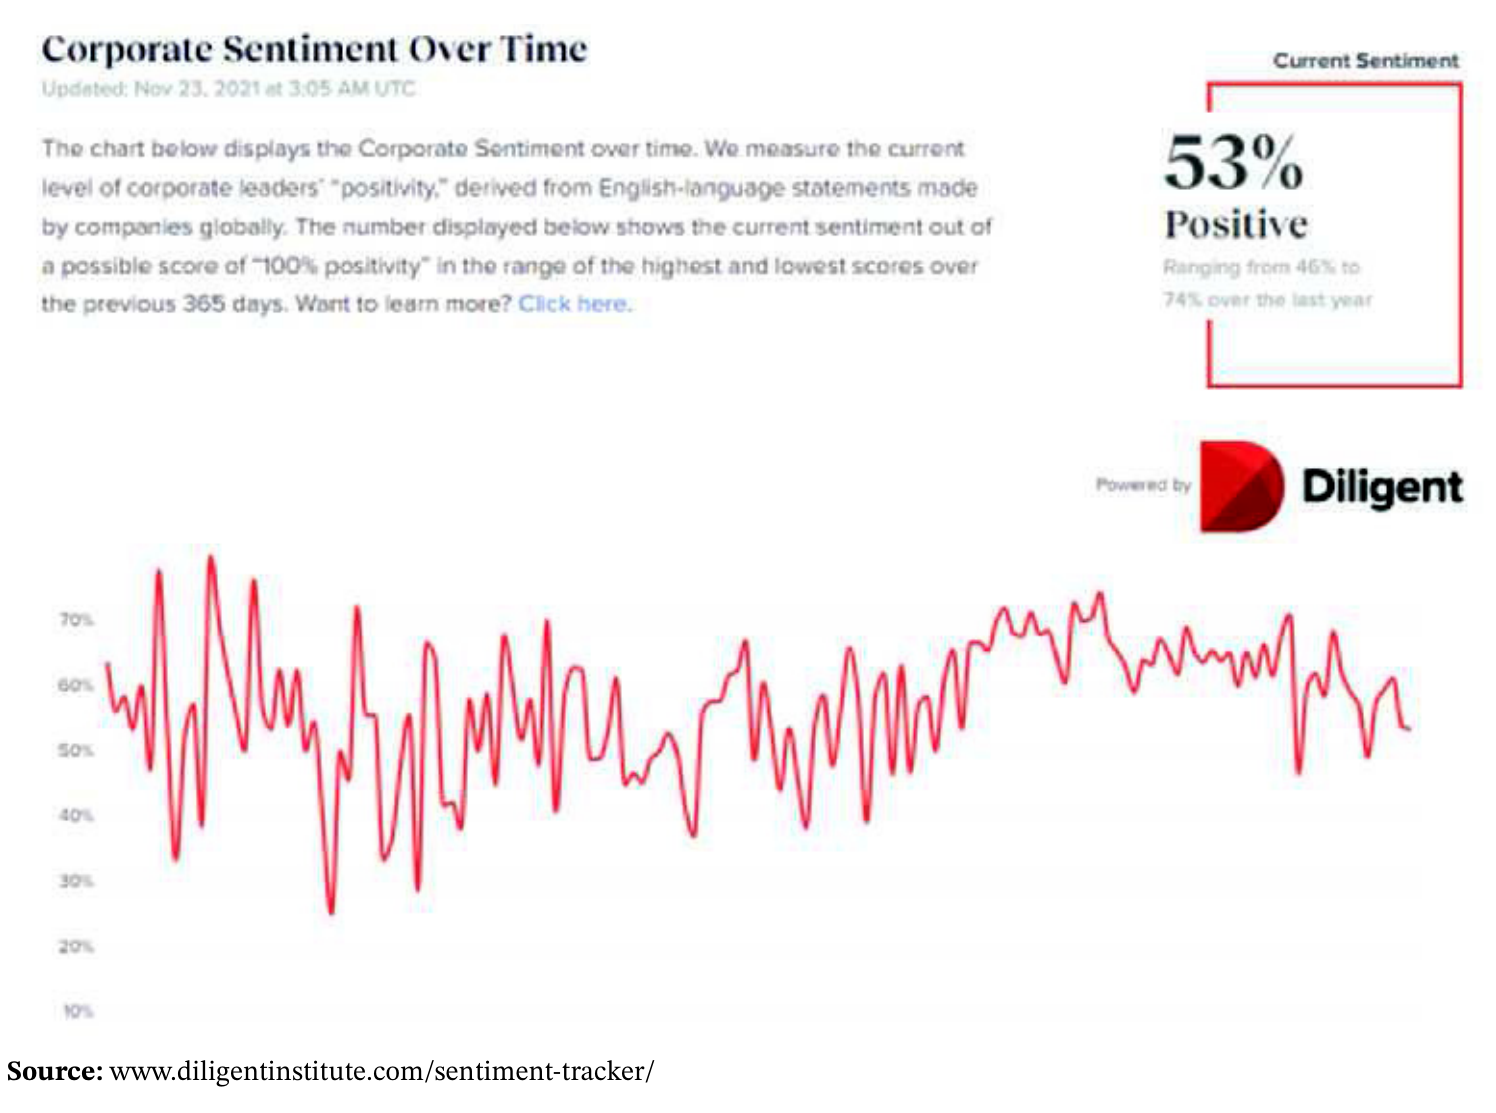
\includegraphics[width=0.95\textwidth,height=0.75\textheight,keepaspectratio]{../textbookForPractice/Figures/Ch_10/ILLUSTRATION 10.19.png}
    \end{figure}
\end{frame}

\begin{frame}{ILLUSTRATION 10.20}

    \begin{figure}[h]
        \centering
        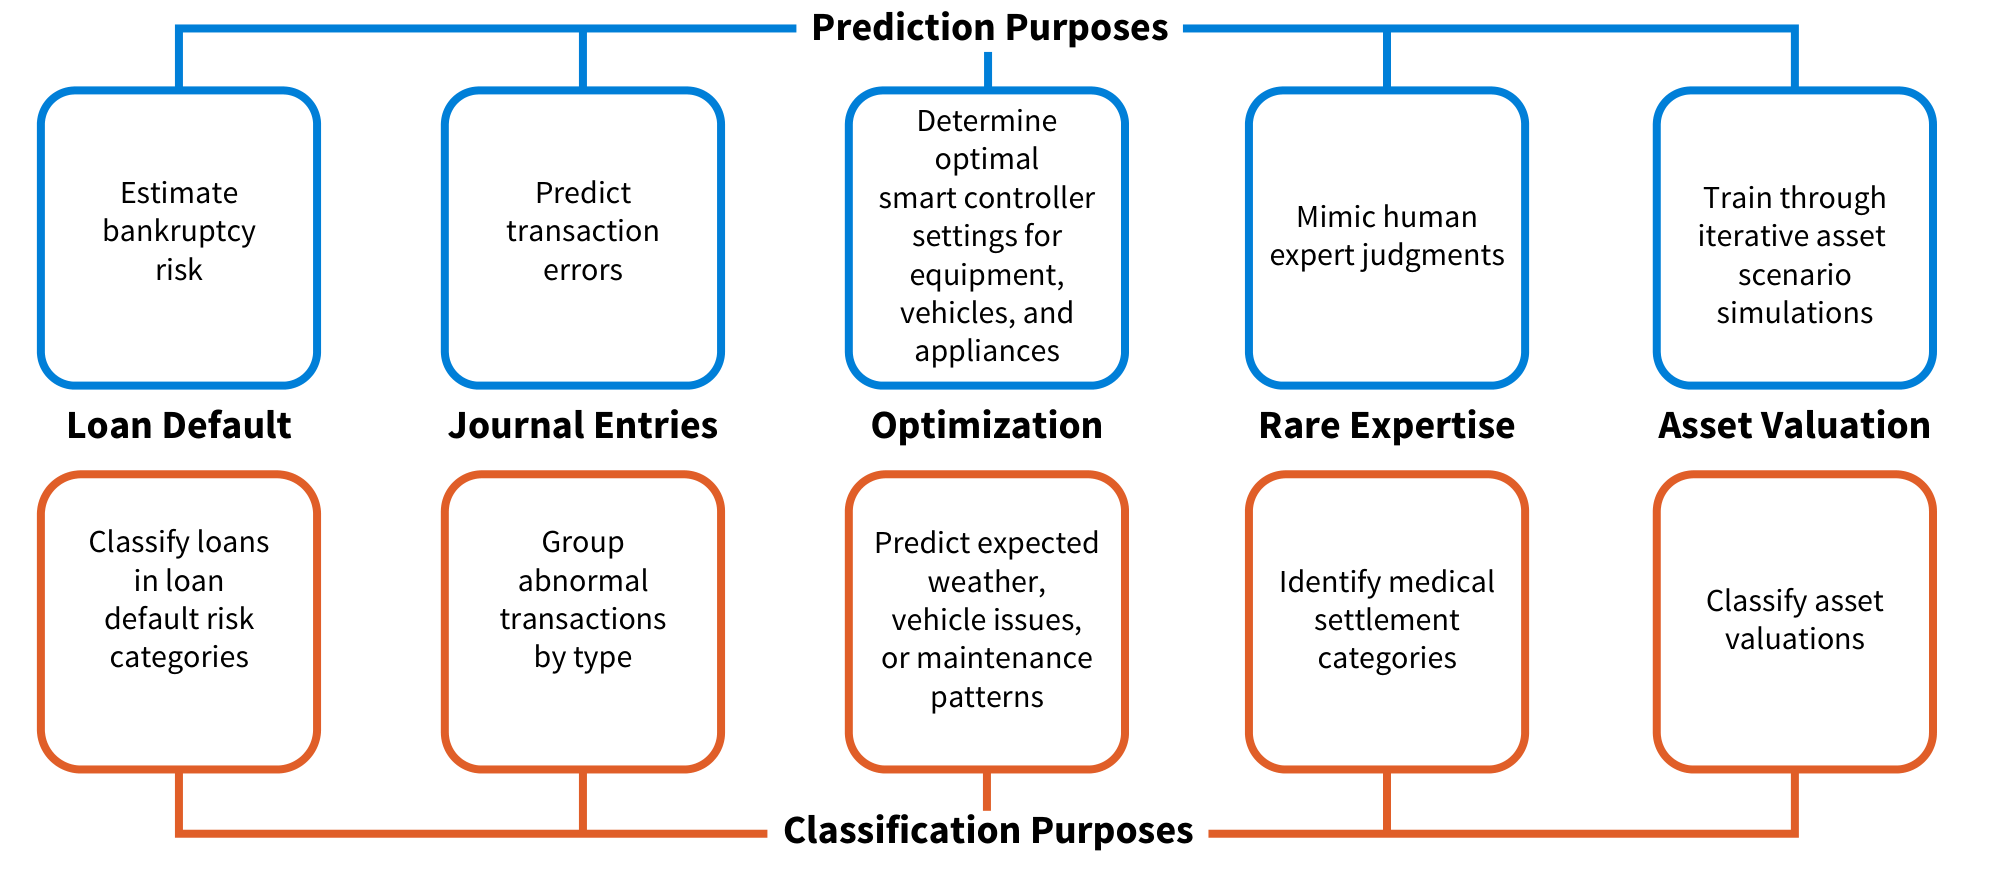
\includegraphics[width=0.95\textwidth,height=0.75\textheight,keepaspectratio]{../textbookForPractice/Figures/Ch_10/ILLUSTRATION 10.20.png}
    \end{figure}
\end{frame}

\begin{frame}{Khai Phá Quy Trình (Process Mining)}
\begin{itemize}
    \item \textbf{Process Mining:} Kỹ thuật phân tích nhật ký sự kiện (event logs) từ hệ thống (ERP) để phát hiện quy trình thực tế diễn ra như thế nào.
    \item \textbf{Ứng dụng:} Tìm ra các điểm nghẽn (bottleneck) trong quy trình phê duyệt tài chính, hoặc các bước thừa thãi gây lãng phí.
\end{itemize}
\end{frame}

\begin{frame}{ILLUSTRATION 10.21}

    \begin{figure}[h]
        \centering
        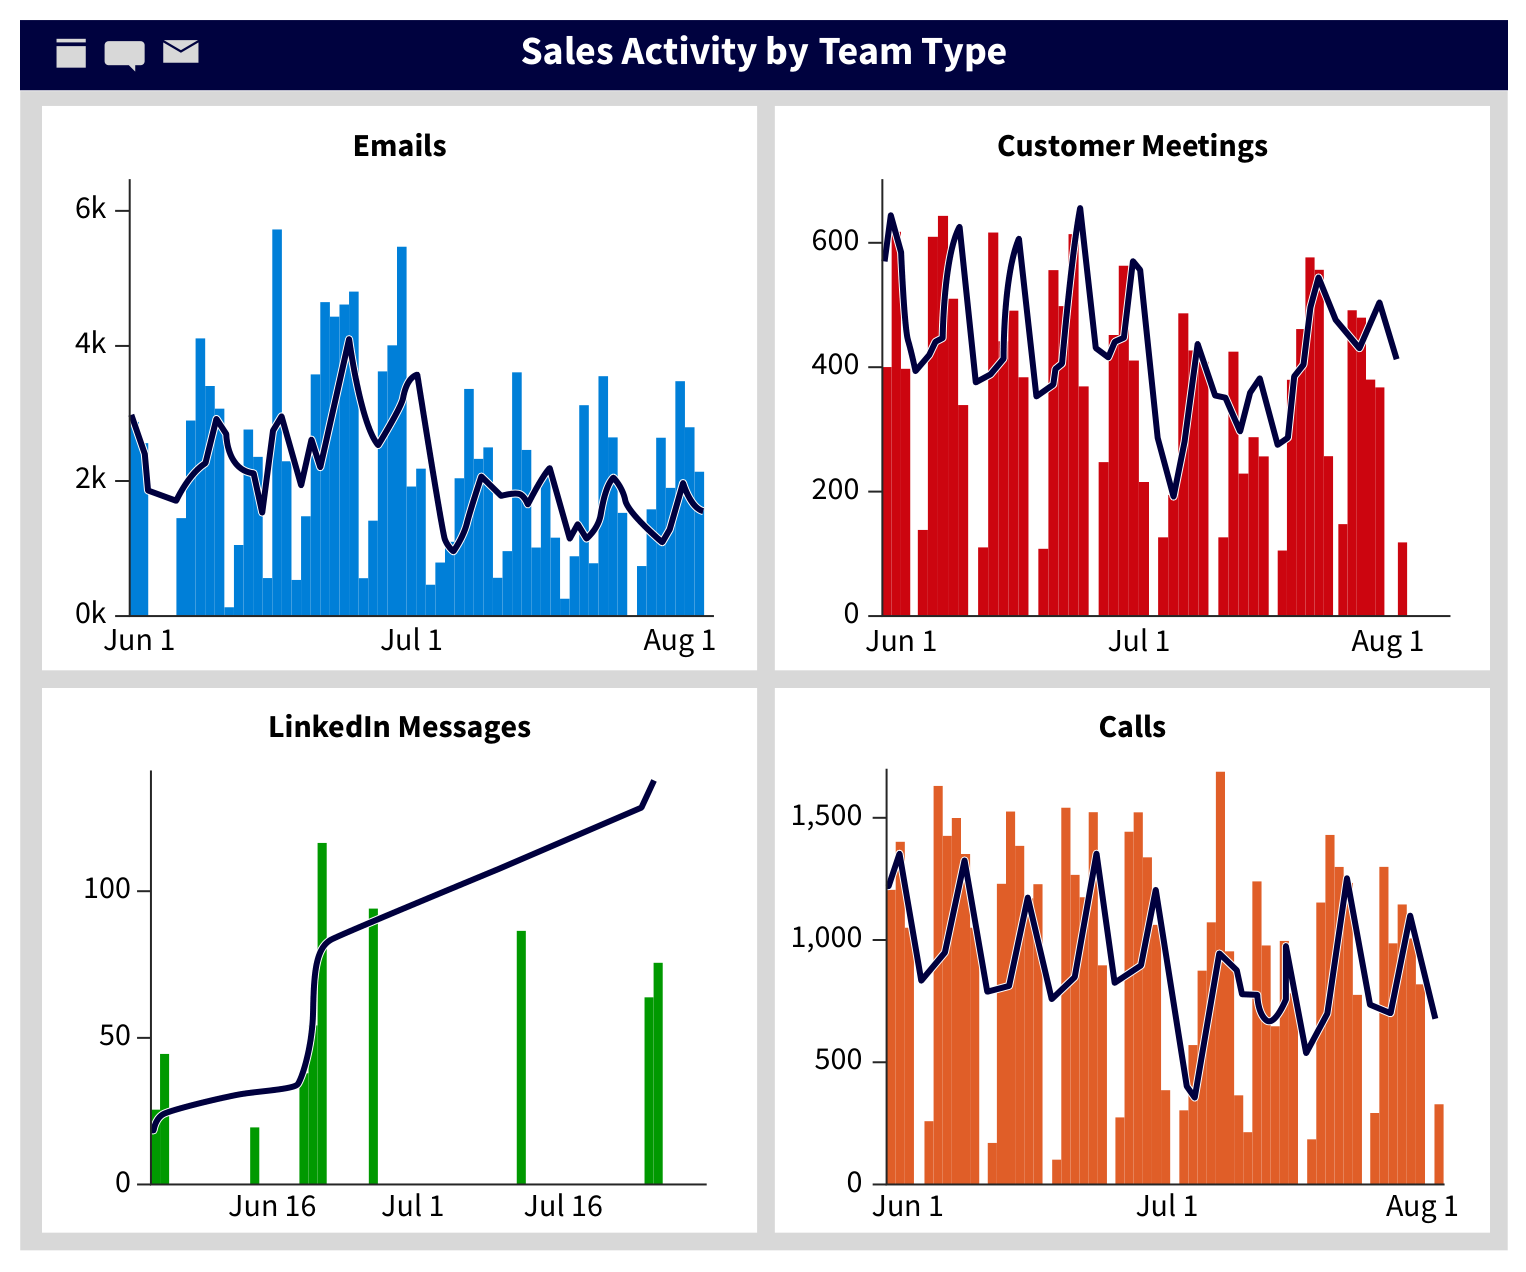
\includegraphics[width=0.95\textwidth,height=0.75\textheight,keepaspectratio]{../textbookForPractice/Figures/Ch_10/ILLUSTRATION 10.21.png}
    \end{figure}
\end{frame}

\begin{frame}{ILLUSTRATION 10.22}

    \begin{figure}[h]
        \centering
        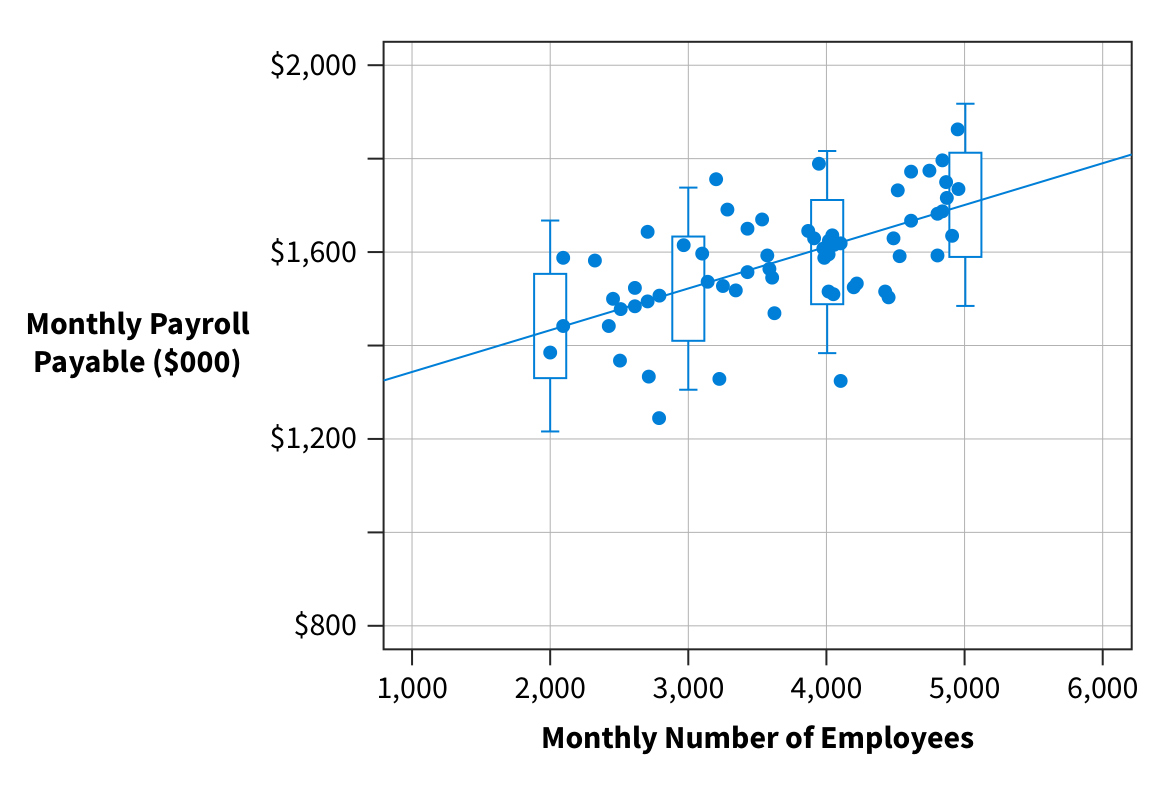
\includegraphics[width=0.95\textwidth,height=0.75\textheight,keepaspectratio]{../textbookForPractice/Figures/Ch_10/ILLUSTRATION 10.22.png}
    \end{figure}
\end{frame}

\begin{frame}{Kiểm Toán Liên Tục (Continuous Auditing)}
\begin{itemize}
    \item \textbf{Khái niệm:} Tự động hóa quá trình giám sát giao dịch tài chính liên tục theo thời gian thực.
    \item \textbf{Cách hoạt động:} Hệ thống cài đặt các ngưỡng báo động (alarms). Bất cứ giao dịch nào vi phạm rule (VD: giao dịch trong ngày nghỉ) sẽ bị đánh dấu ngay lập tức.
\end{itemize}
\end{frame}

\begin{frame}{ILLUSTRATION 10.23}

    \begin{figure}[h]
        \centering
        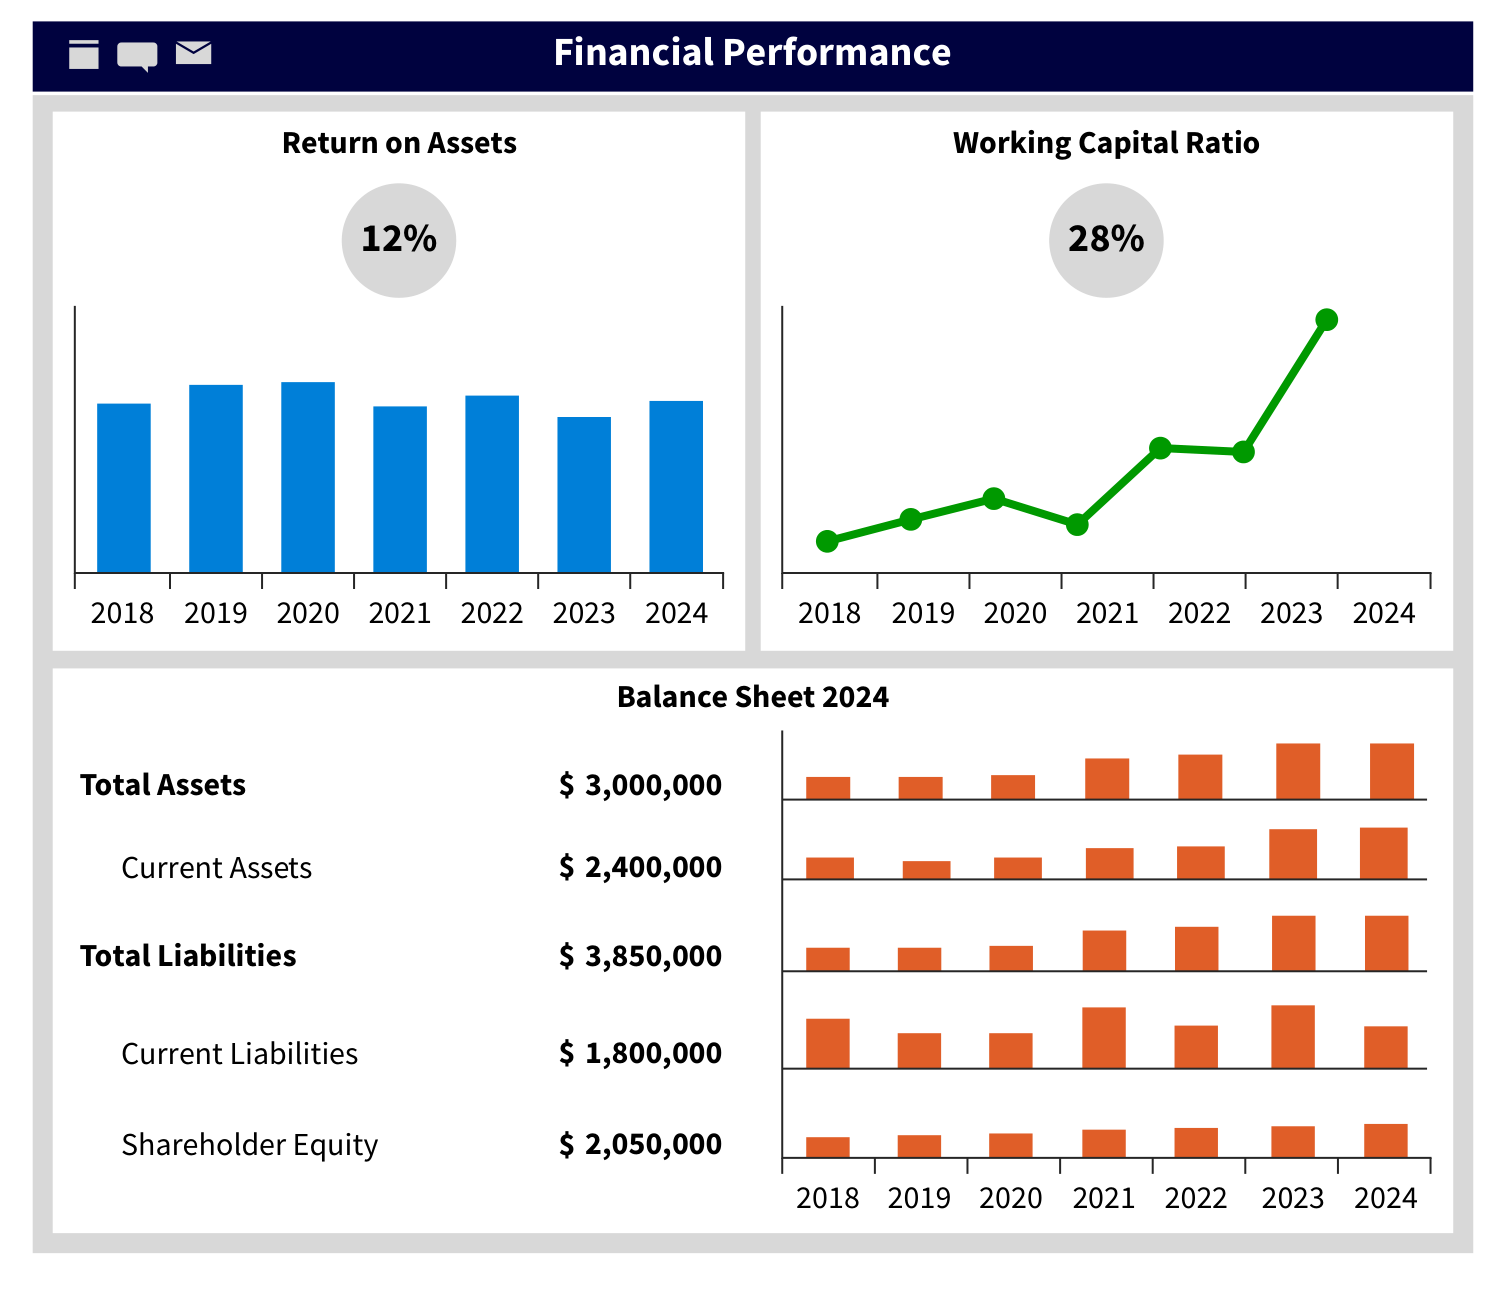
\includegraphics[width=0.95\textwidth,height=0.75\textheight,keepaspectratio]{../textbookForPractice/Figures/Ch_10/ILLUSTRATION 10.23.png}
    \end{figure}
\end{frame}

\begin{frame}{ILLUSTRATION 10.24}

    \begin{figure}[h]
        \centering
        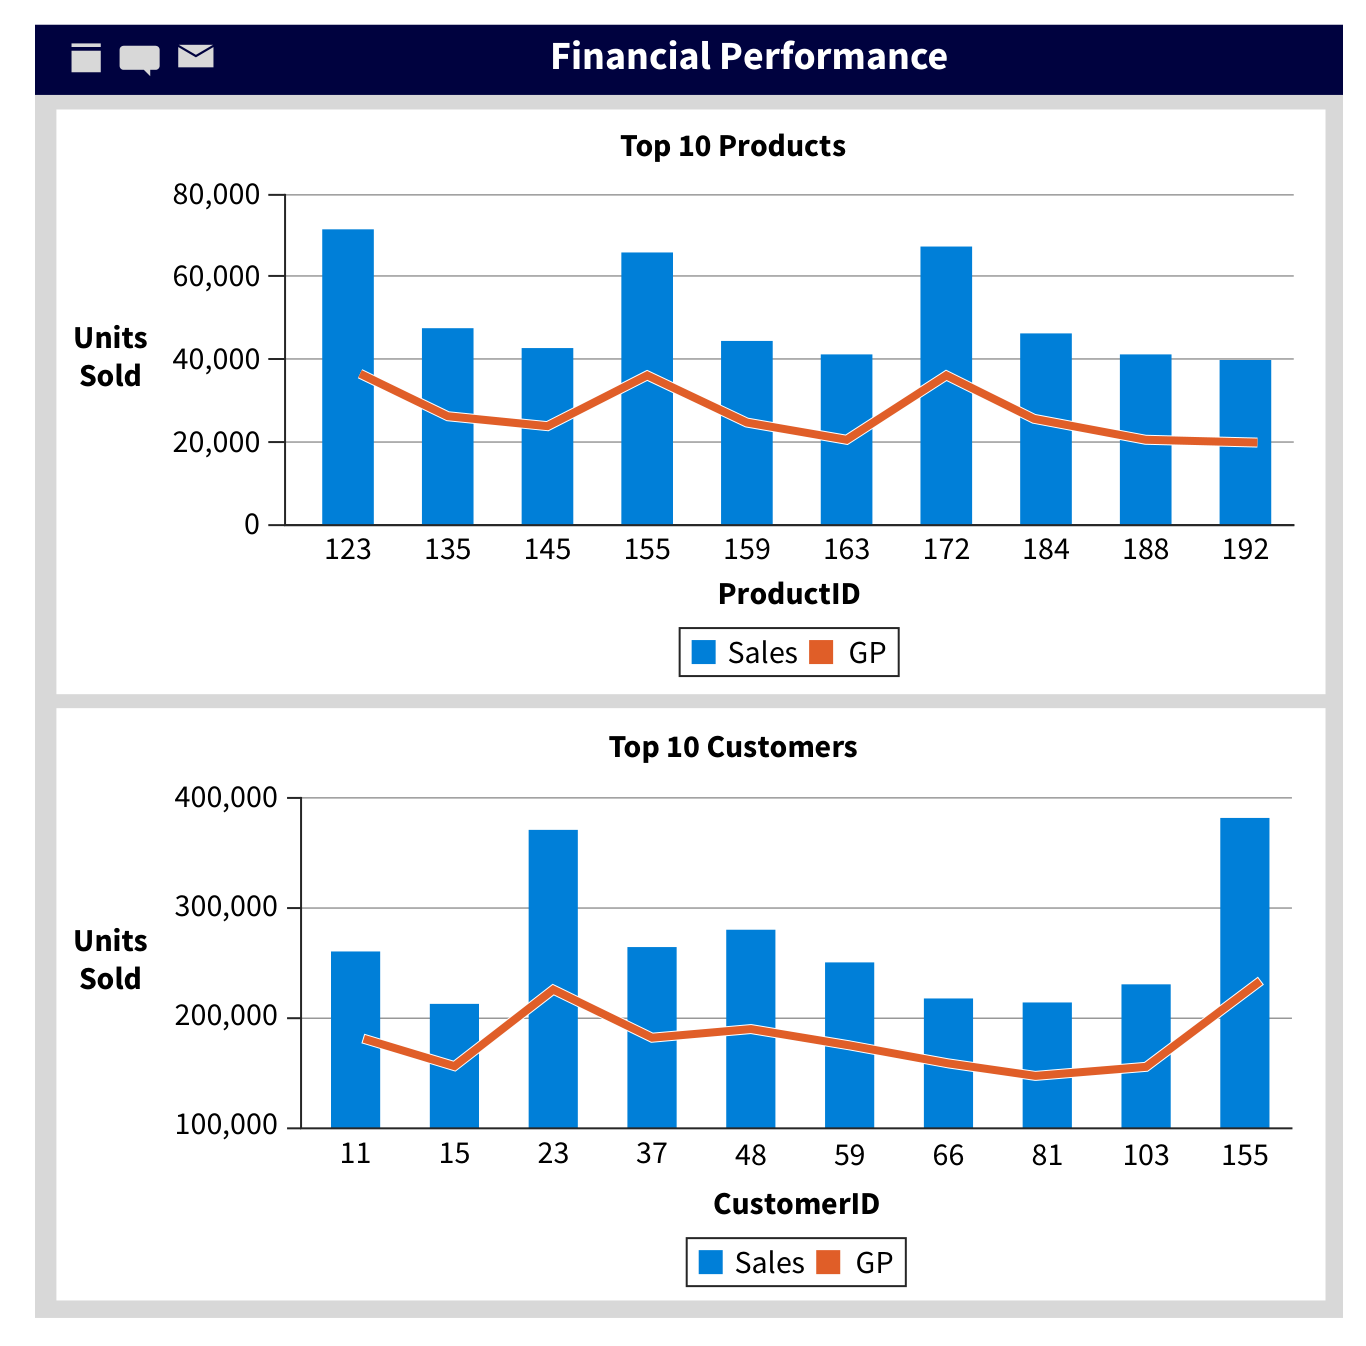
\includegraphics[width=0.95\textwidth,height=0.75\textheight,keepaspectratio]{../textbookForPractice/Figures/Ch_10/ILLUSTRATION 10.24.png}
    \end{figure}
\end{frame}

\begin{frame}{Phân Tích Văn Bản (Textual Analysis)}
\begin{itemize}
    \item \textbf{Textual Analysis:} Sử dụng NLP (Xử lý ngôn ngữ tự nhiên) để trích xuất thông tin từ tài liệu phi cấu trúc (Báo cáo thường niên 10-K, Biên bản họp).
    \item \textbf{Phân tích cảm xúc (Sentiment Analysis):} Đo lường tông giọng lạc quan hay bi quan của Ban giám đốc để dự báo hiệu quả tương lai.
\end{itemize}
\end{frame}

\begin{frame}{ILLUSTRATION 10.25}

    \begin{figure}[h]
        \centering
        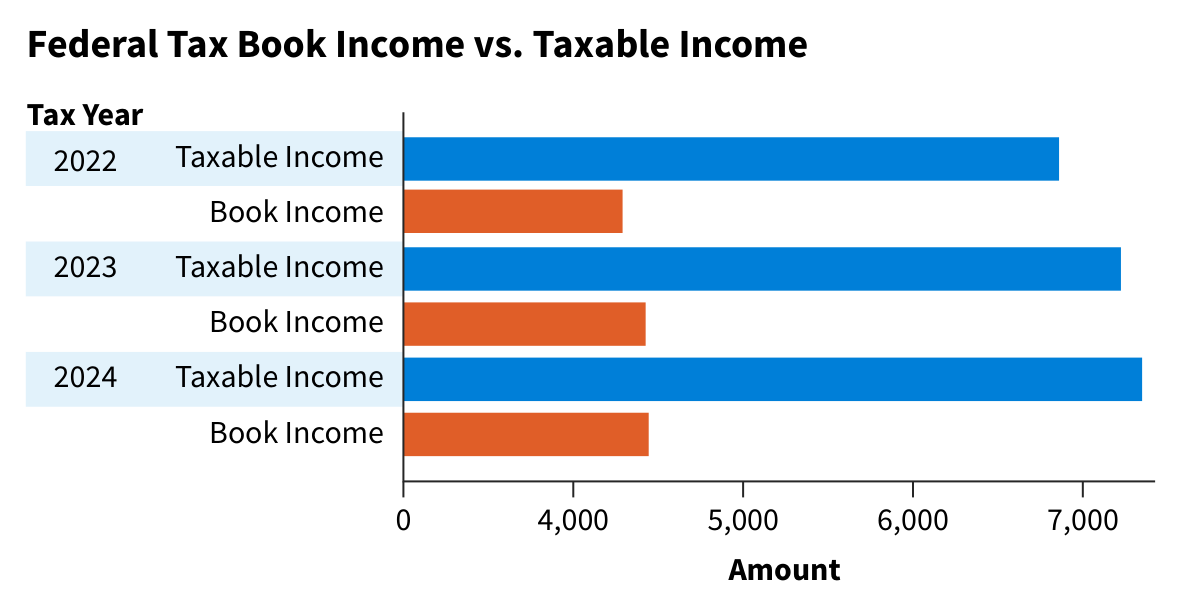
\includegraphics[width=0.95\textwidth,height=0.75\textheight,keepaspectratio]{../textbookForPractice/Figures/Ch_10/ILLUSTRATION 10.25.png}
    \end{figure}
\end{frame}

\begin{frame}{ILLUSTRATION 10.26}

    \begin{figure}[h]
        \centering
        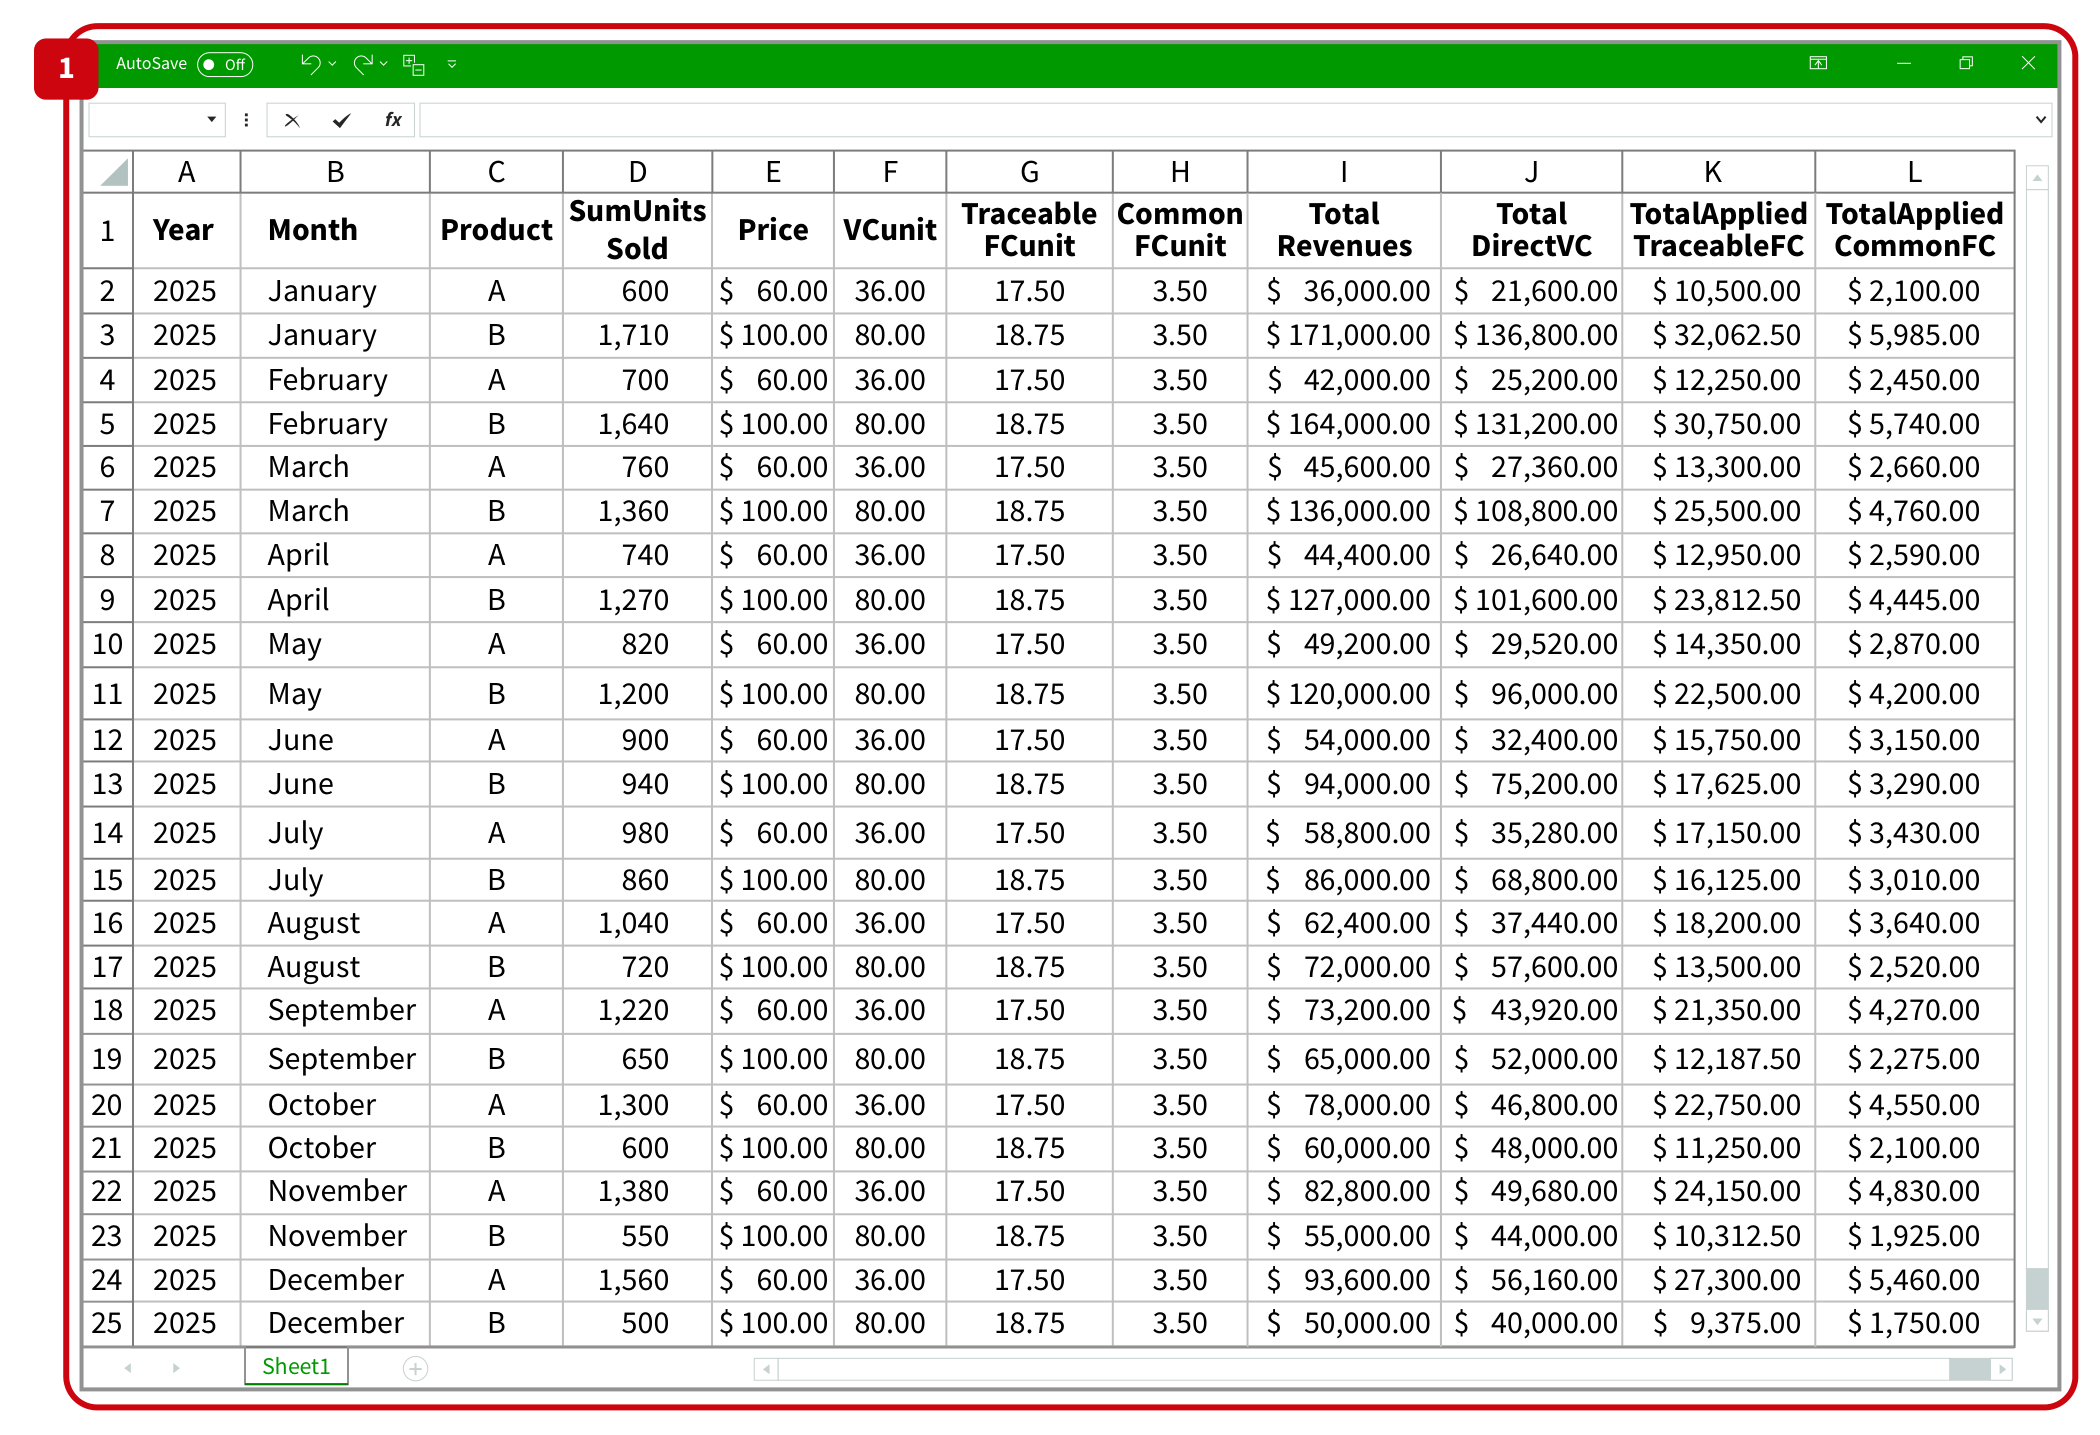
\includegraphics[width=0.95\textwidth,height=0.75\textheight,keepaspectratio]{../textbookForPractice/Figures/Ch_10/ILLUSTRATION 10.26.png}
    \end{figure}
\end{frame}

\begin{frame}{Trí Tuệ Nhân Tạo (AI) \& Công Nghệ Nhận Thức}
\begin{itemize}
    \item \textbf{Công nghệ nhận thức (Cognitive Technologies):} Giúp phần mềm có khả năng nhìn (Computer Vision), nghe, đọc và đưa ra quyết định như con người.
    \item \textbf{Machine Learning (Học máy):} Thuật toán có khả năng tự cải thiện theo thời gian mà không cần lập trình lại tường minh (VD: Nhận diện chứng từ giả).
\end{itemize}
\end{frame}

\begin{frame}{ILLUSTRATION 10.27}

    \begin{figure}[h]
        \centering
        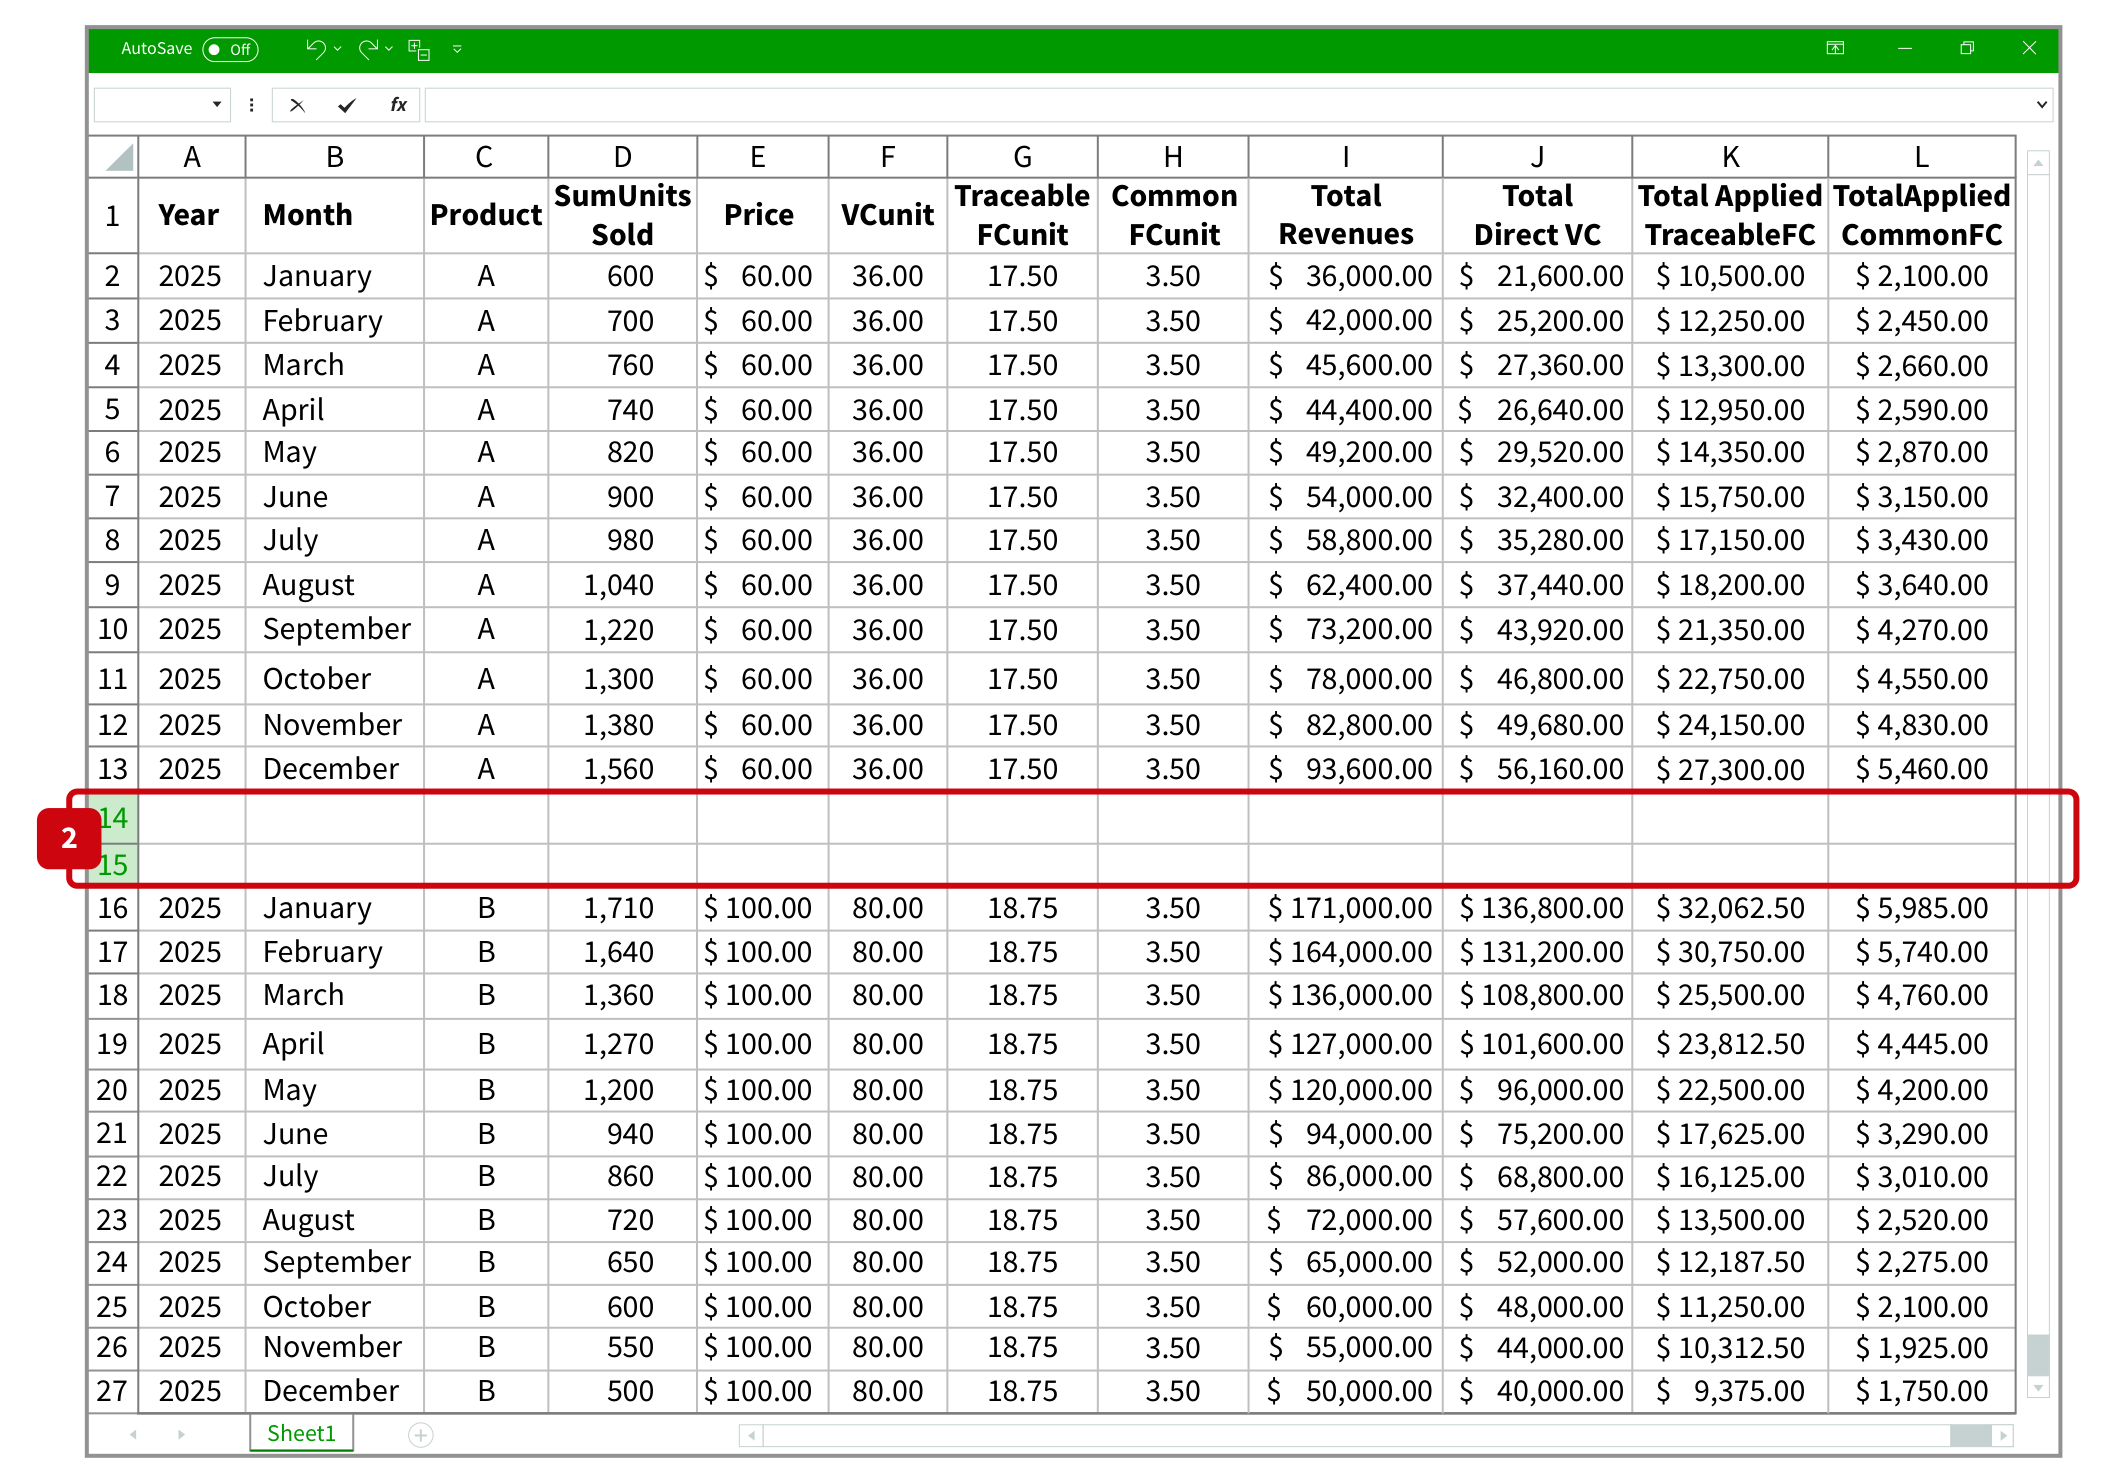
\includegraphics[width=0.95\textwidth,height=0.75\textheight,keepaspectratio]{../textbookForPractice/Figures/Ch_10/ILLUSTRATION 10.27.png}
    \end{figure}
\end{frame}

\begin{frame}{ILLUSTRATION 10.28}

    \begin{figure}[h]
        \centering
        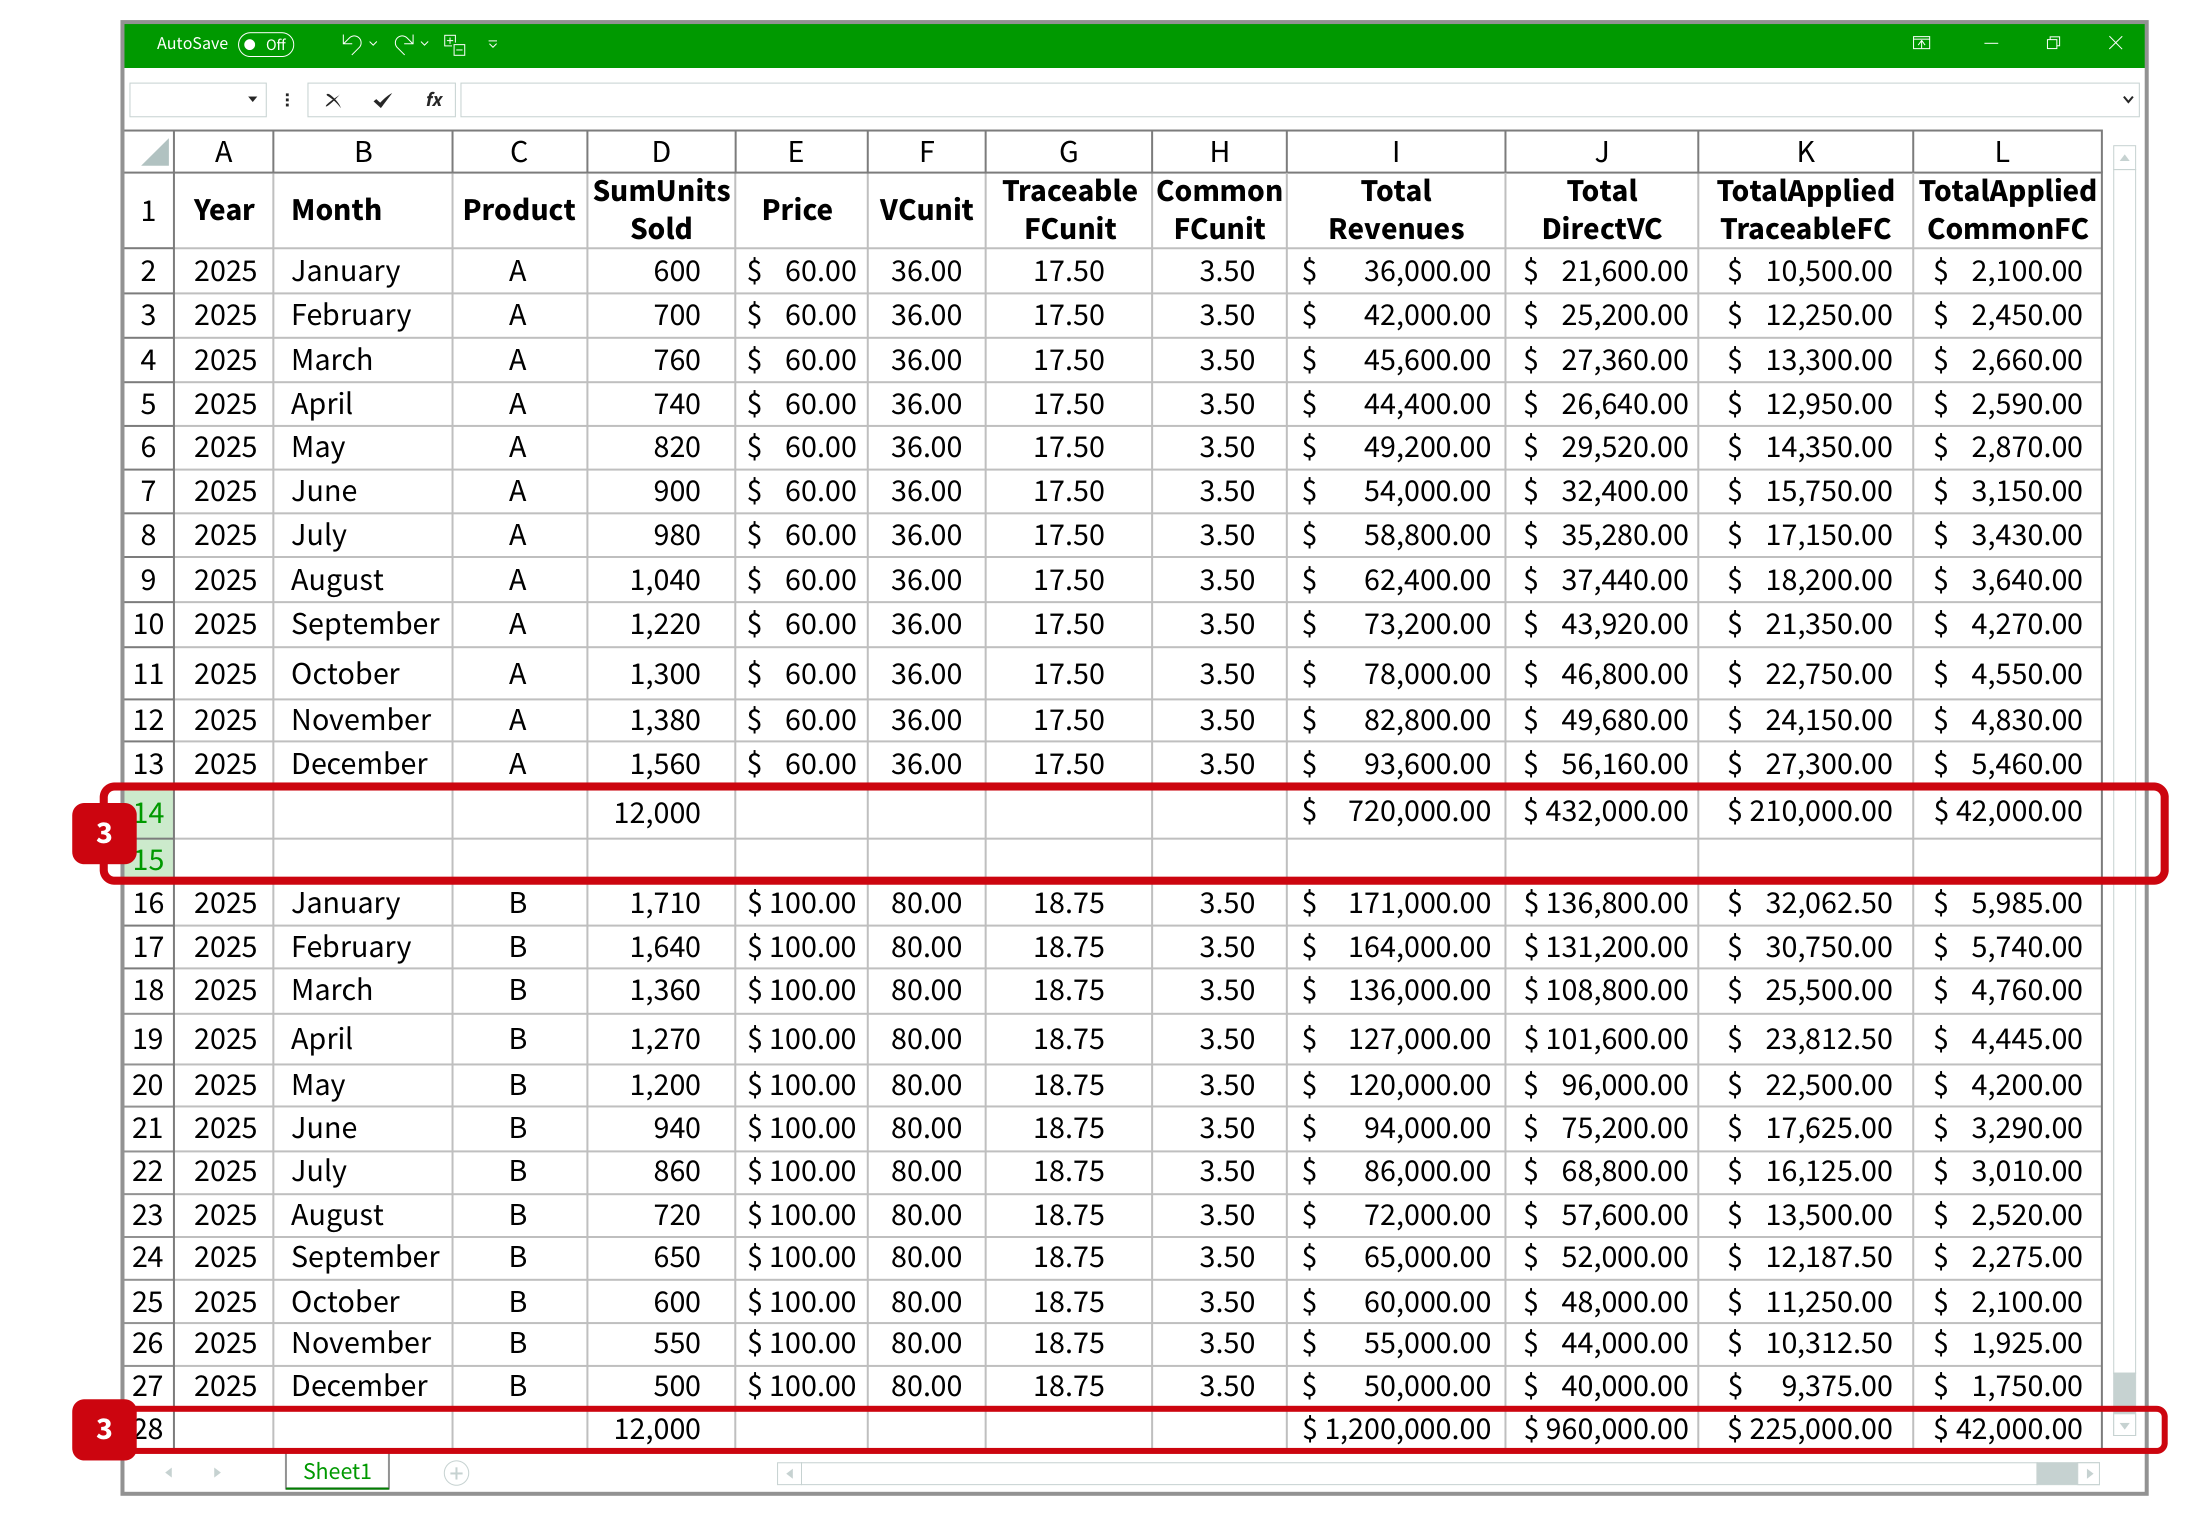
\includegraphics[width=0.95\textwidth,height=0.75\textheight,keepaspectratio]{../textbookForPractice/Figures/Ch_10/ILLUSTRATION 10.28.png}
    \end{figure}
\end{frame}

\begin{frame}{10.3 Công Nghệ Gia Tăng Giá Trị Kế Toán}
\begin{itemize}
    \item Sự thay đổi diễn ra ở tất cả các lĩnh vực cốt lõi của ngành:
    \begin{itemize}
        \item Hệ thống Thông tin Kế toán (AIS)
        \item Kiểm toán (Auditing)
        \item Kế toán Tài chính (Financial Accounting)
        \item Kế toán Quản trị (Managerial Accounting)
        \item Kế toán Thuế (Tax Accounting)
    \end{itemize}
\end{itemize}
\end{frame}

\begin{frame}{ILLUSTRATION 10.29}

    \begin{figure}[h]
        \centering
        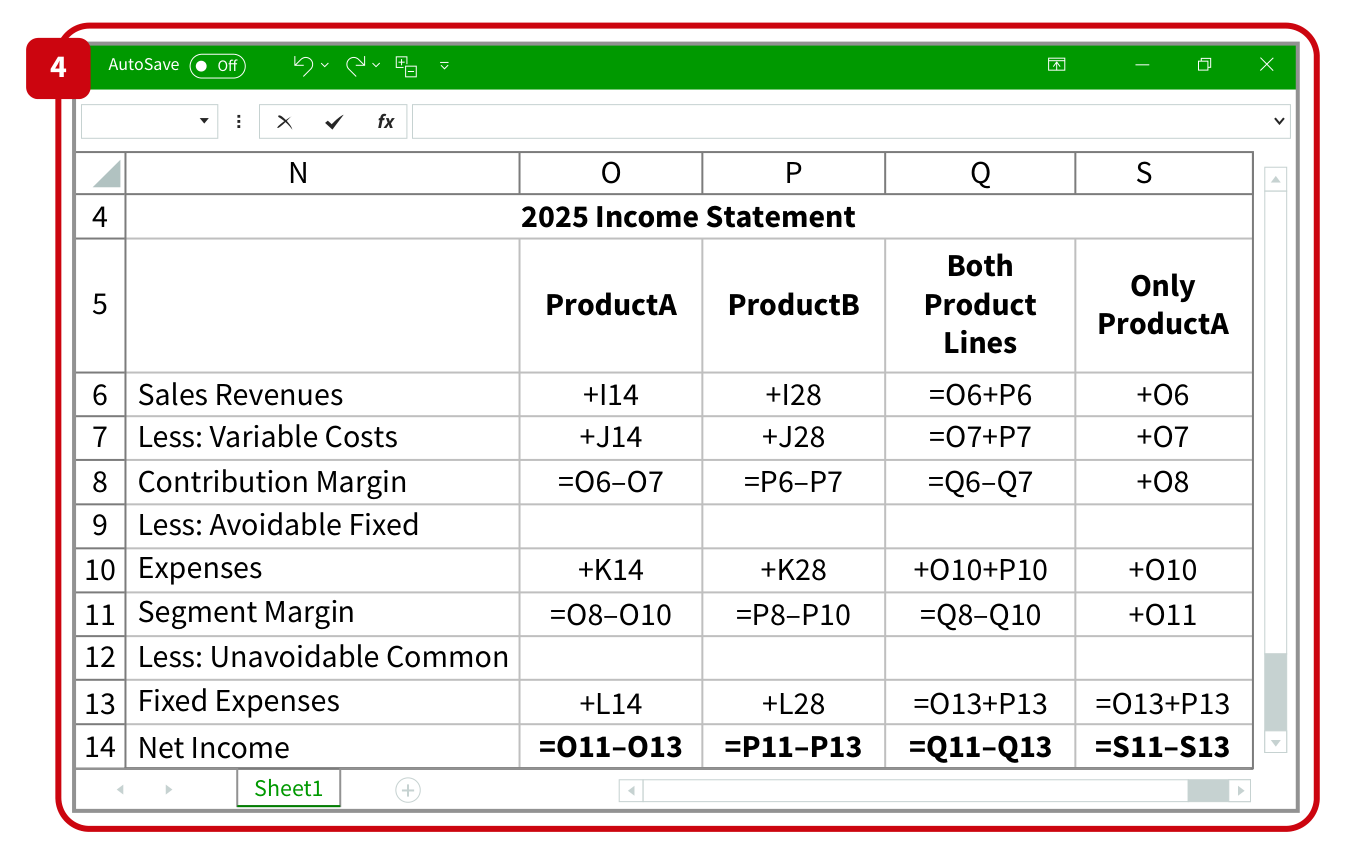
\includegraphics[width=0.95\textwidth,height=0.75\textheight,keepaspectratio]{../textbookForPractice/Figures/Ch_10/ILLUSTRATION 10.29.png}
    \end{figure}
\end{frame}

\begin{frame}{ILLUSTRATION 10.30}

    \begin{figure}[h]
        \centering
        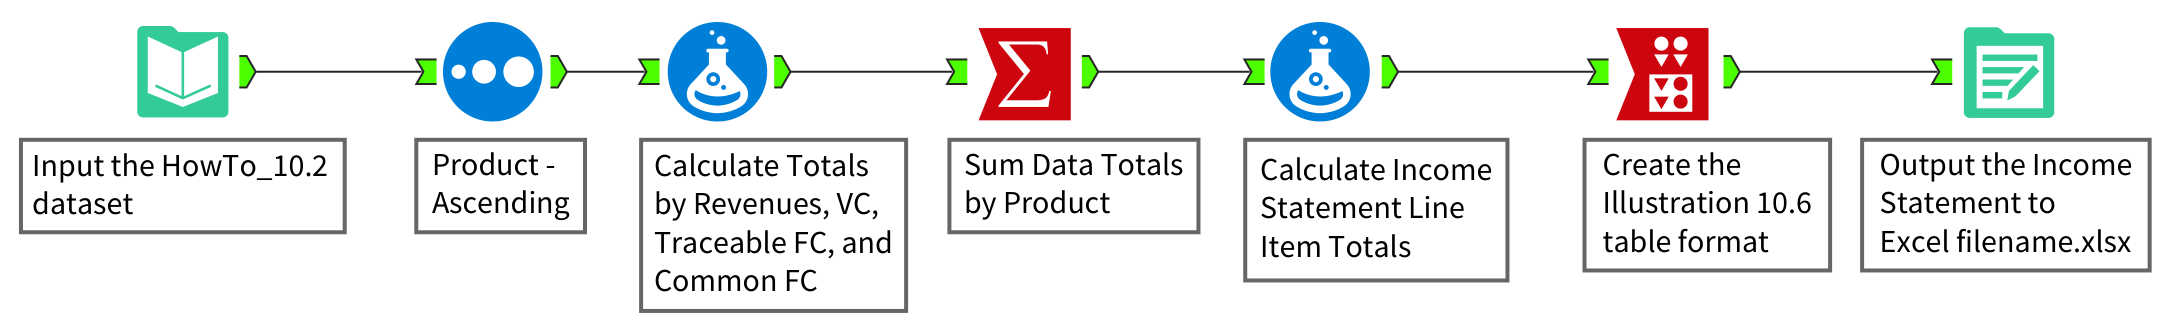
\includegraphics[width=0.95\textwidth,height=0.75\textheight,keepaspectratio]{../textbookForPractice/Figures/Ch_10/ILLUSTRATION 10.30.png}
    \end{figure}
\end{frame}

\begin{frame}{Hệ thống Thông tin Kế toán (AIS)}
\begin{itemize}
    \item Hệ thống ERP hiện đại (như SAP, Oracle) đã tích hợp sẵn AI.
    \item \textbf{Vai trò của Kế toán:} Trở thành người giám sát, đảm bảo chất lượng dữ liệu đầu vào và thiết lập các rule chuẩn cho RPA tự động chạy.
\end{itemize}
\end{frame}

\begin{frame}{ILLUSTRATION 10.31}

    \begin{figure}[h]
        \centering
        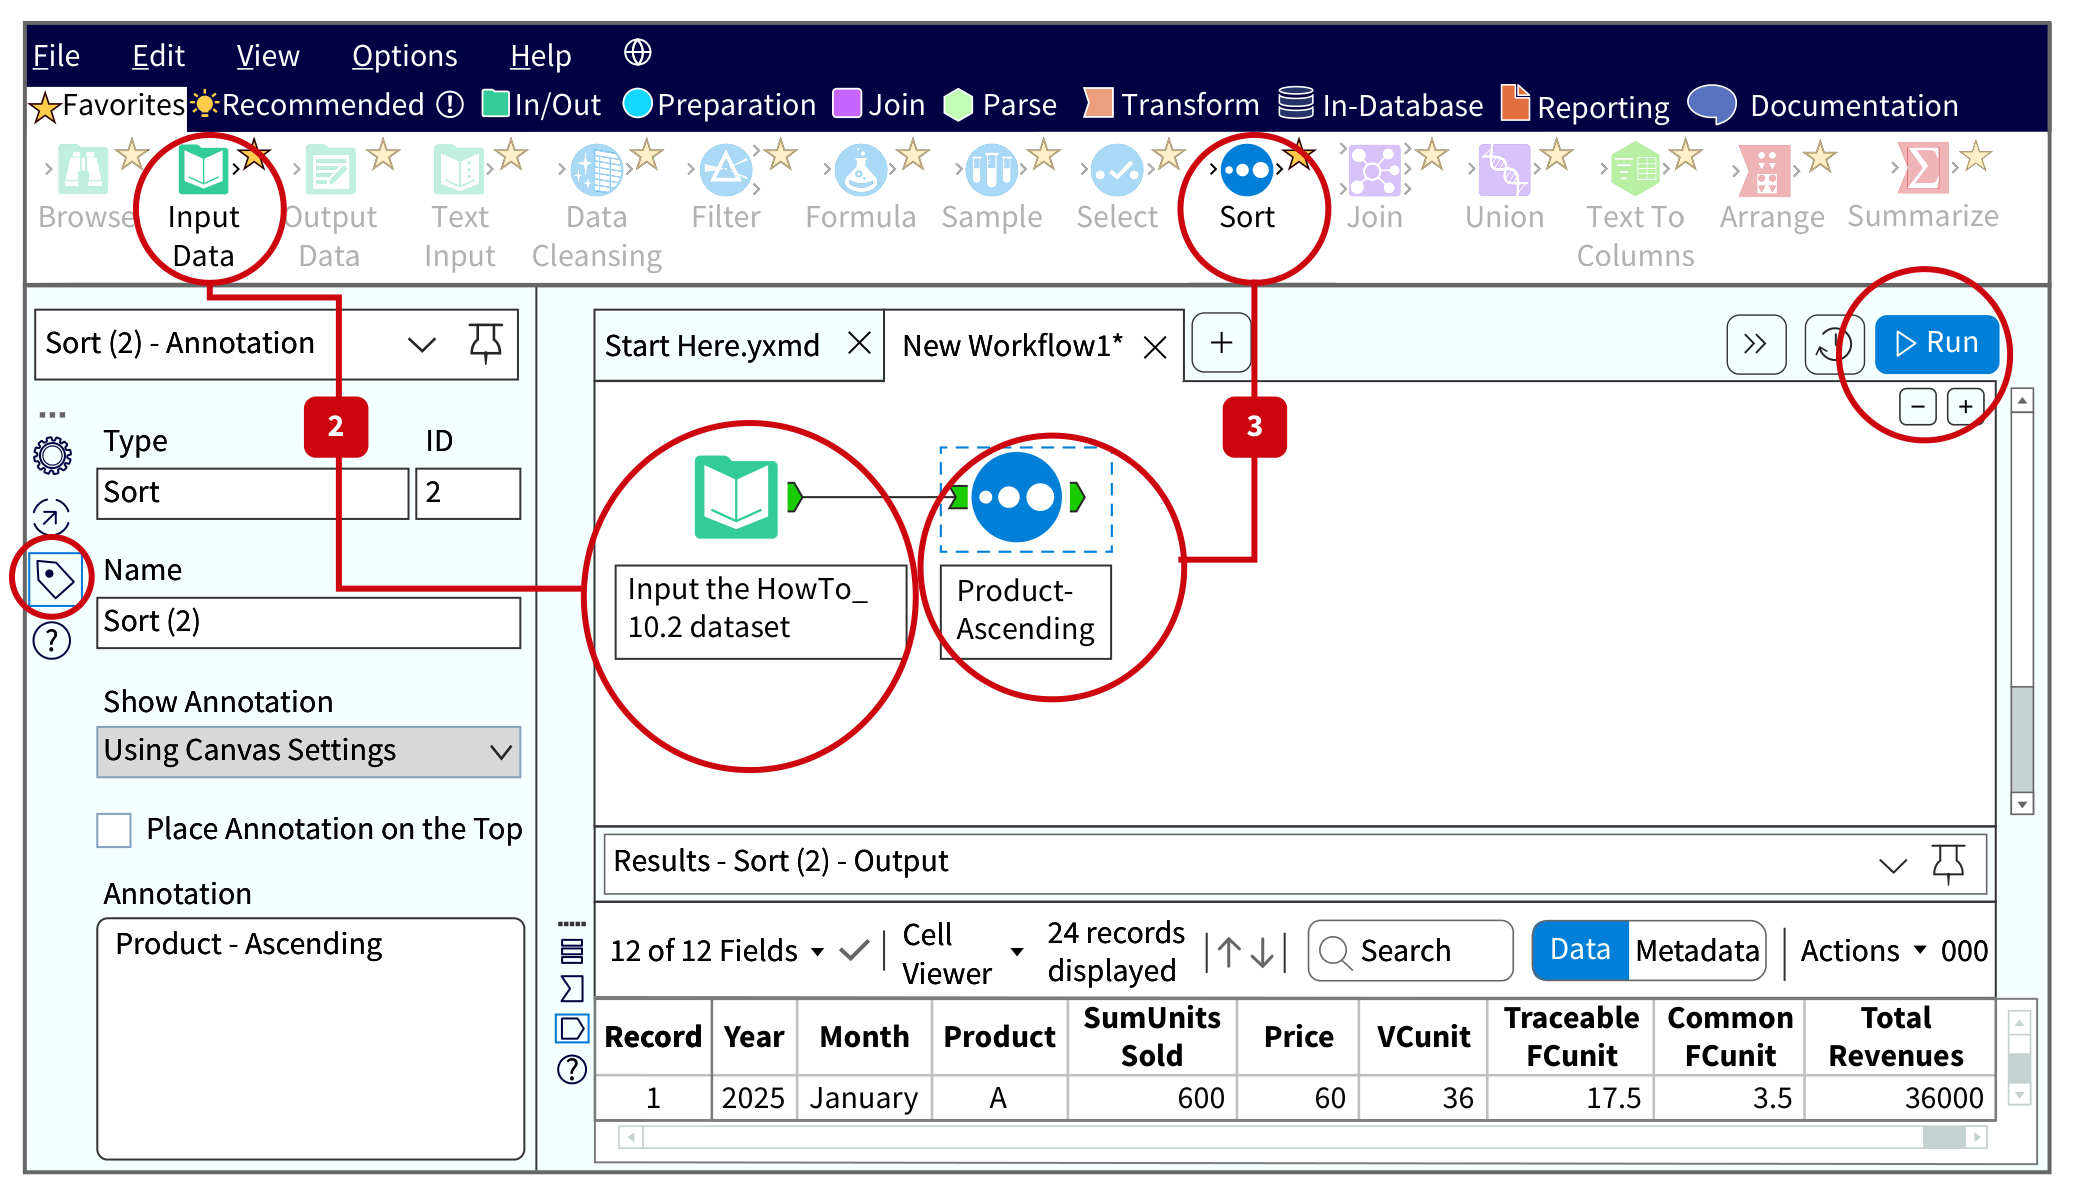
\includegraphics[width=0.95\textwidth,height=0.75\textheight,keepaspectratio]{../textbookForPractice/Figures/Ch_10/ILLUSTRATION 10.31.png}
    \end{figure}
\end{frame}

\begin{frame}{ILLUSTRATION 10.32}

    \begin{figure}[h]
        \centering
        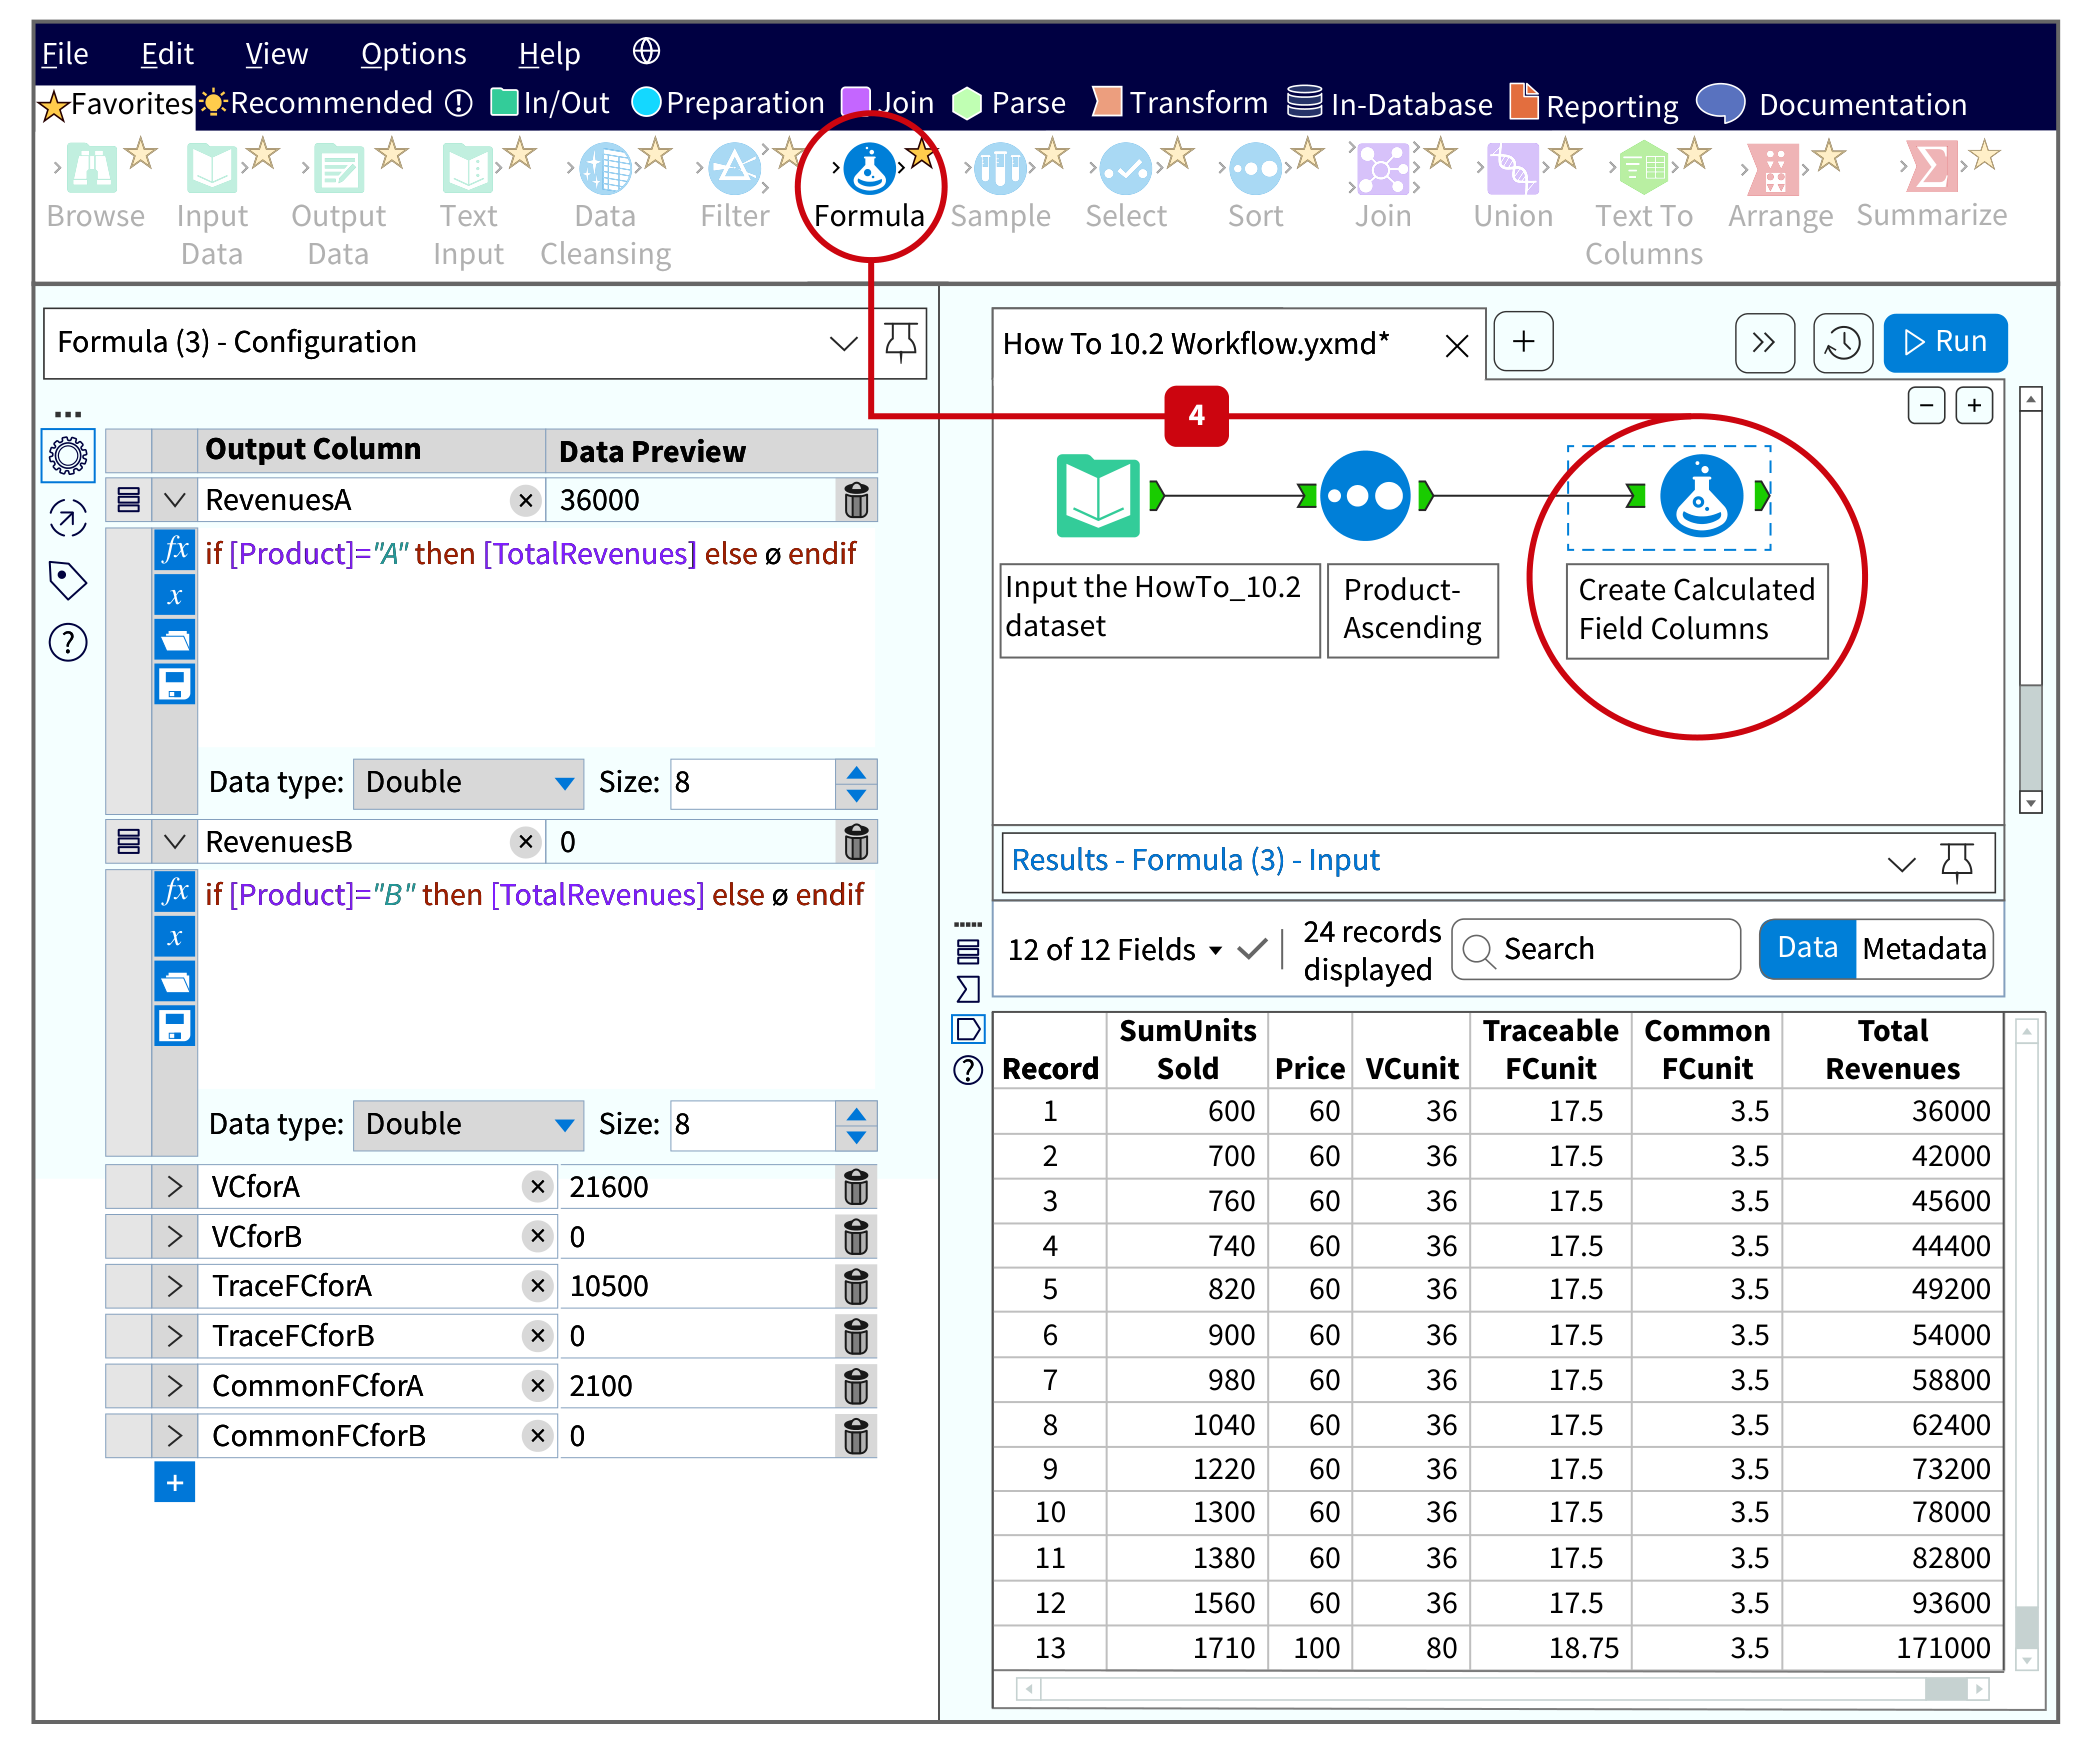
\includegraphics[width=0.95\textwidth,height=0.75\textheight,keepaspectratio]{../textbookForPractice/Figures/Ch_10/ILLUSTRATION 10.32.png}
    \end{figure}
\end{frame}

\begin{frame}{Kiểm toán (Auditing)}
\begin{itemize}
    \item Không còn kiểm tra chọn mẫu. Phân tích dữ liệu cho phép kiểm tra 100\% tổng thể dữ liệu giao dịch.
    \item Nhận diện rủi ro chủ động bằng học máy thay vì phản ứng thụ động sau khi kỳ kế toán kết thúc.
\end{itemize}
\end{frame}

\begin{frame}{ILLUSTRATION 10.33}

    \begin{figure}[h]
        \centering
        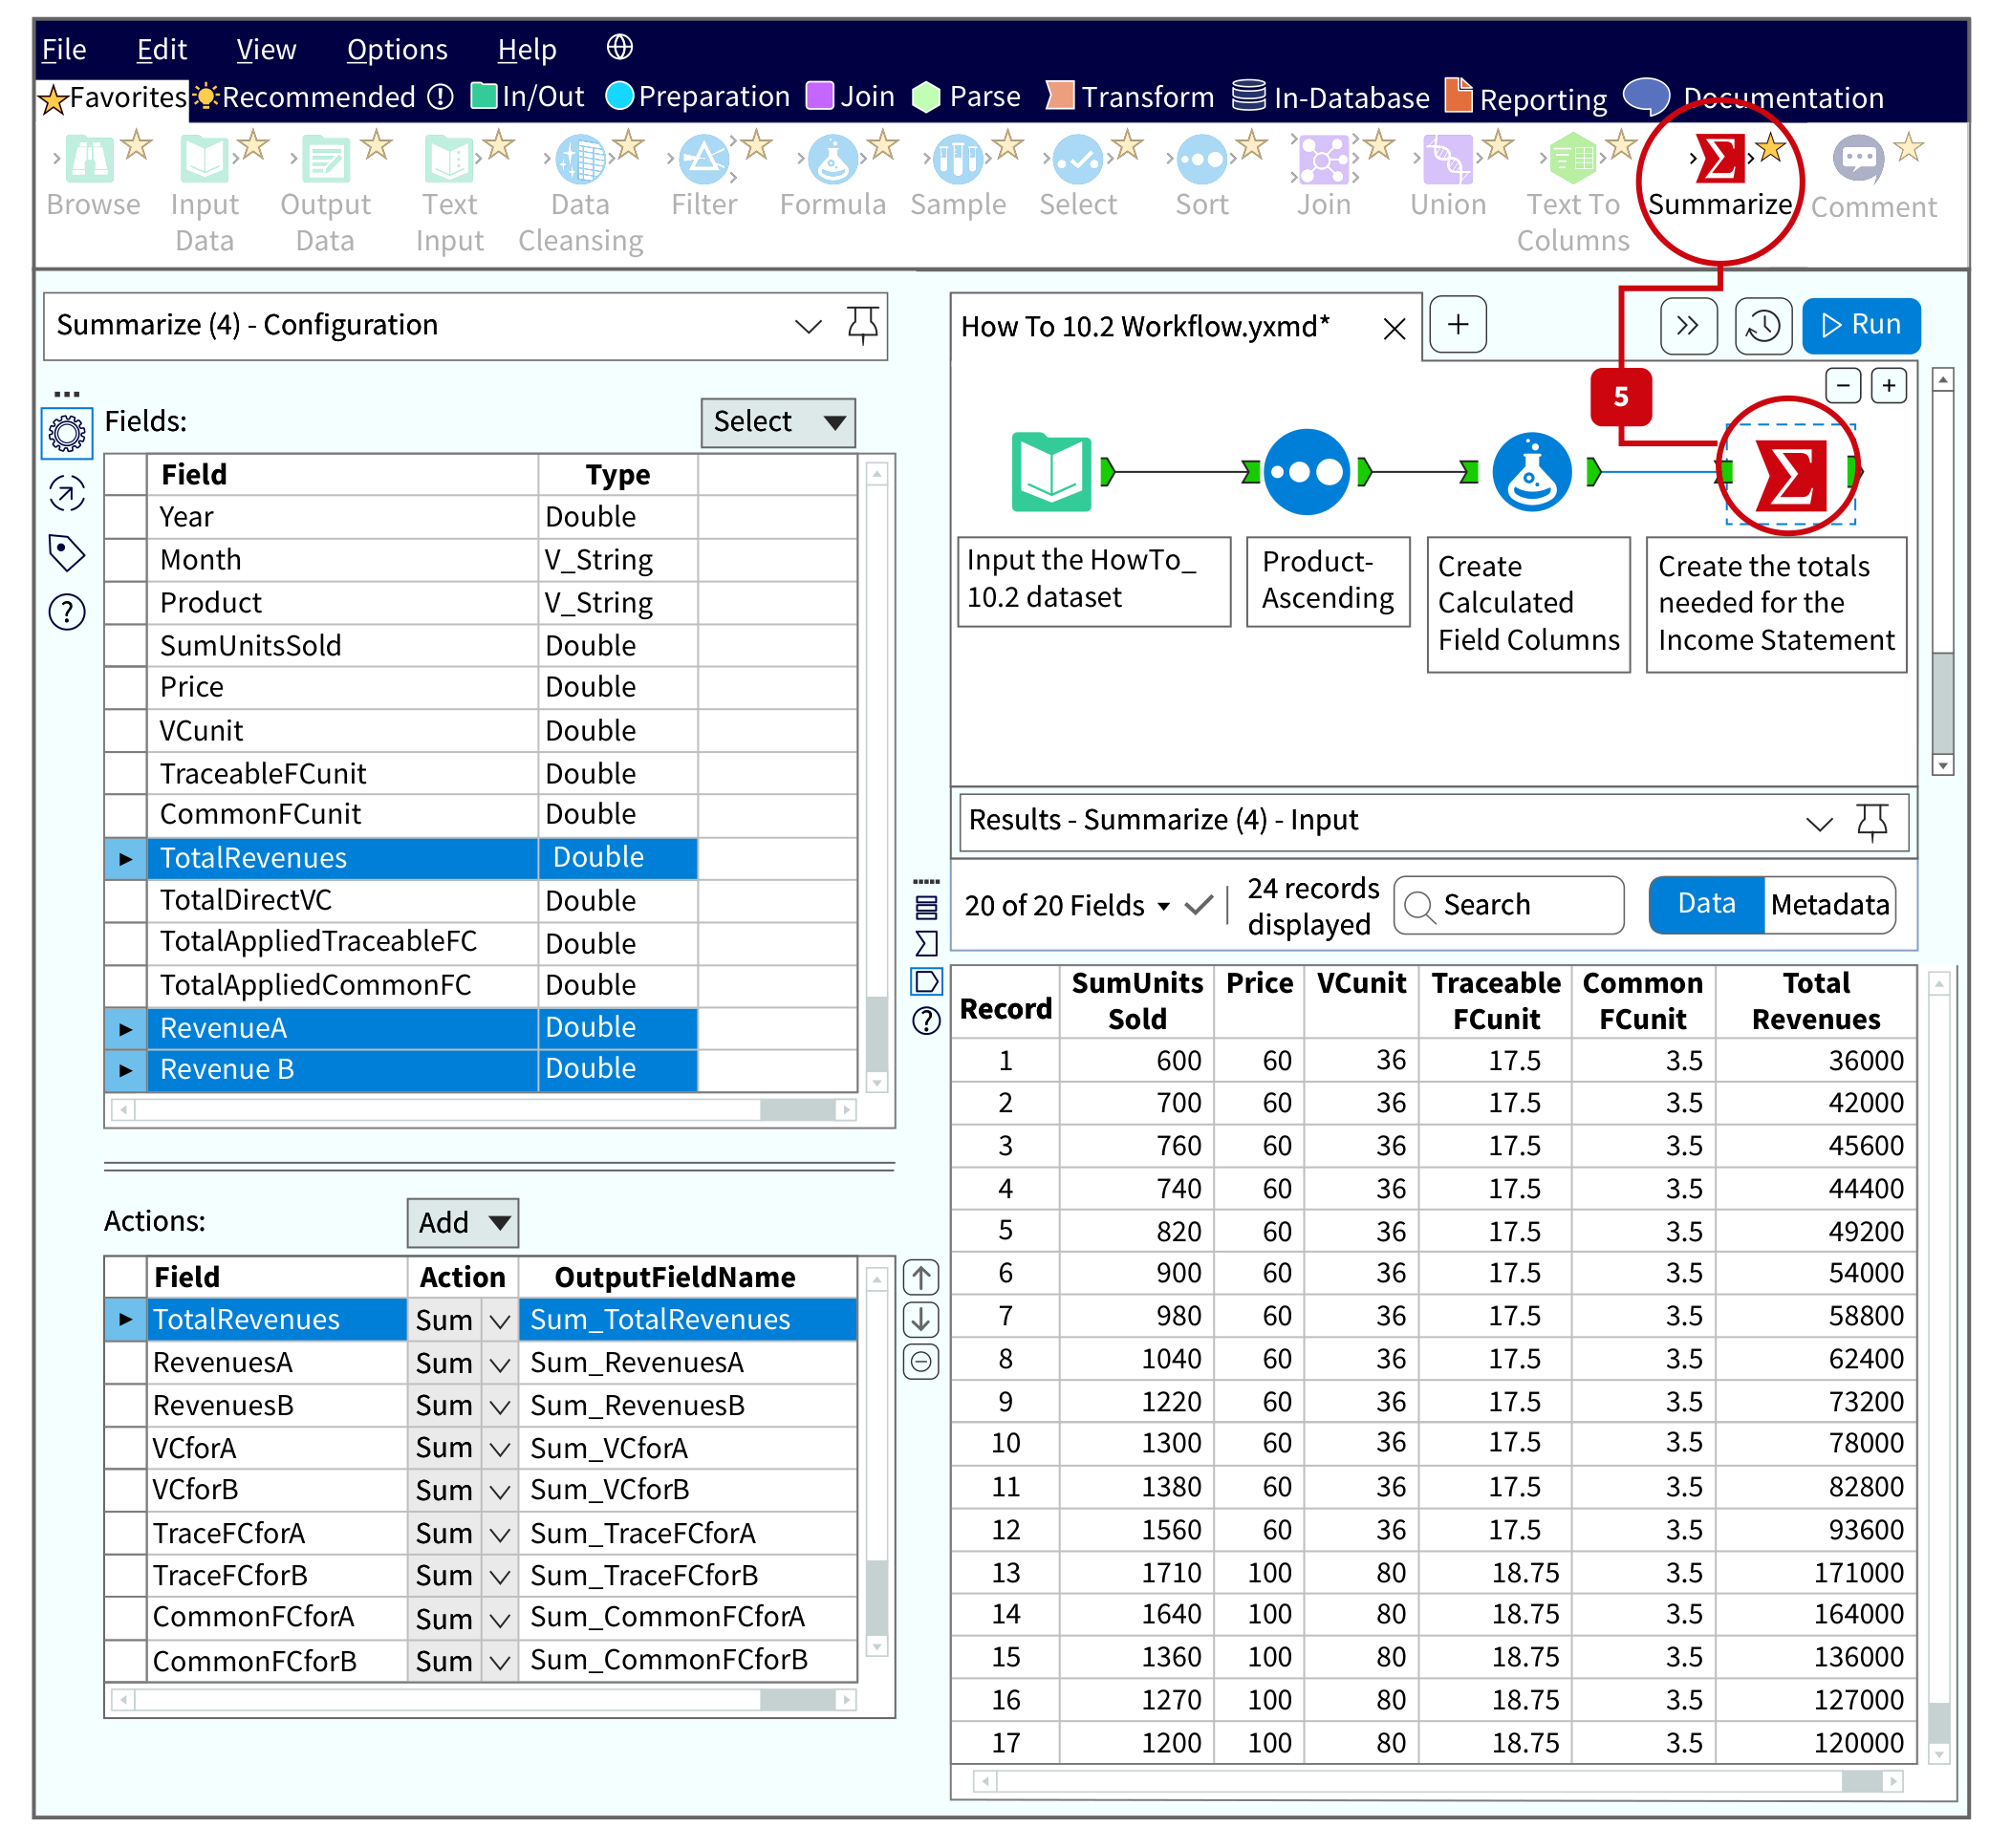
\includegraphics[width=0.95\textwidth,height=0.75\textheight,keepaspectratio]{../textbookForPractice/Figures/Ch_10/ILLUSTRATION 10.33.png}
    \end{figure}
\end{frame}

\begin{frame}{ILLUSTRATION 10.34}

    \begin{figure}[h]
        \centering
        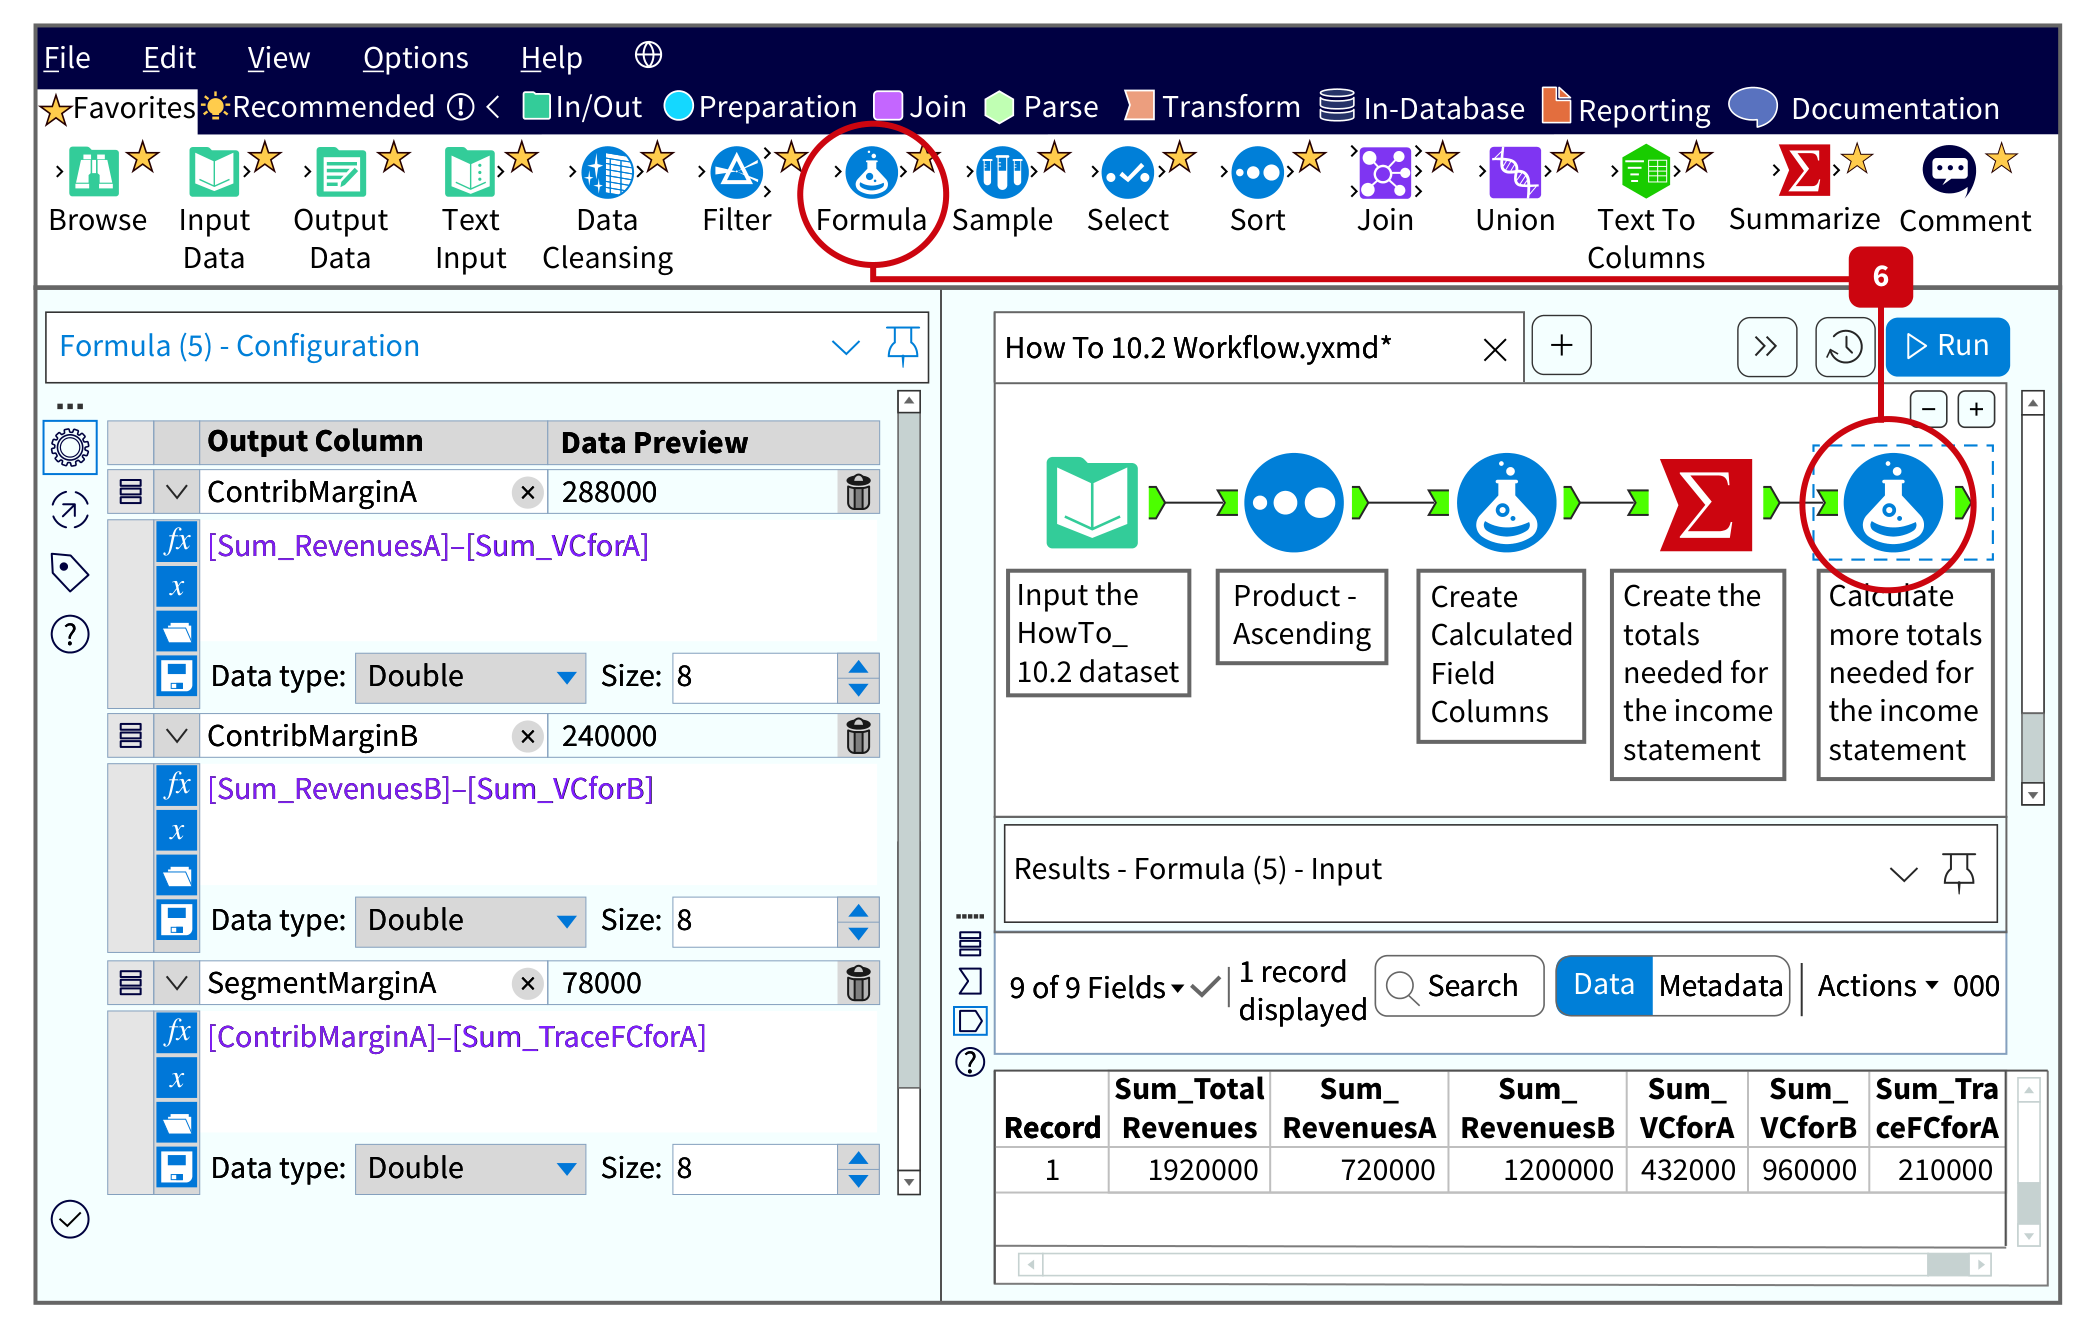
\includegraphics[width=0.95\textwidth,height=0.75\textheight,keepaspectratio]{../textbookForPractice/Figures/Ch_10/ILLUSTRATION 10.34.png}
    \end{figure}
\end{frame}

\begin{frame}{Kế toán Tài chính}
\begin{itemize}
    \item Phân tích văn bản trên hàng ngàn BCTC 10-K của đối thủ trong vài giây để đưa ra báo cáo so sánh.
    \item Hỗ trợ lập BCTC chuẩn XBRL tự động và phát hiện bất thường trước khi nộp lên Ủy ban Chứng khoán.
\end{itemize}
\end{frame}

\begin{frame}{ILLUSTRATION 10.35A}

    \begin{figure}[h]
        \centering
        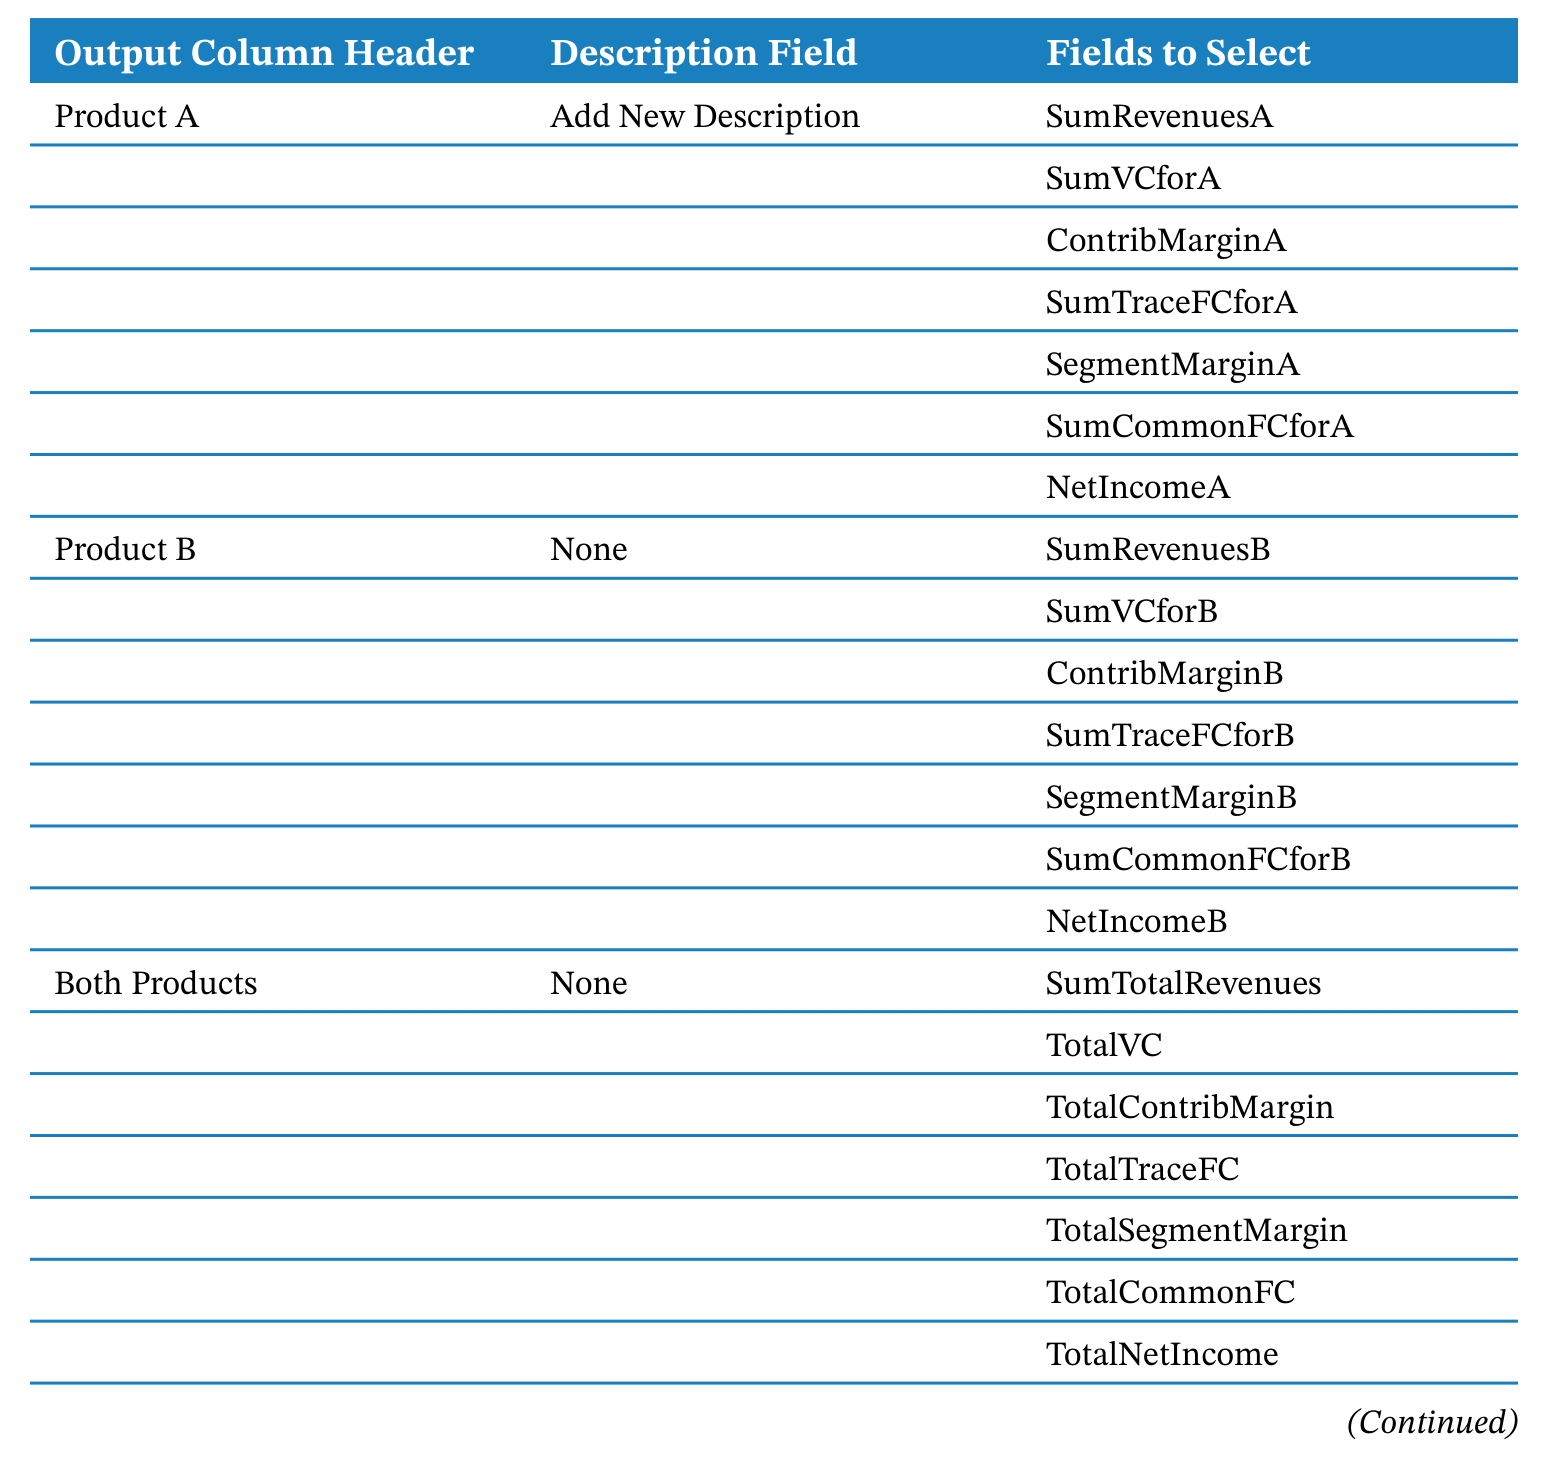
\includegraphics[width=0.95\textwidth,height=0.75\textheight,keepaspectratio]{../textbookForPractice/Figures/Ch_10/ILLUSTRATION 10.35A.png}
    \end{figure}
\end{frame}

\begin{frame}{Kế toán Quản trị}
\begin{itemize}
    \item Thay vì chỉ nhìn vào quá khứ (Descriptive), Kế toán Quản trị chuyển sang Dự báo (Predictive) và Đề xuất (Prescriptive).
    \item Ứng dụng Process Mining để tối ưu hóa chi phí vận hành chuỗi cung ứng.
\end{itemize}
\end{frame}

\begin{frame}{ILLUSTRATION 10.35B}

    \begin{figure}[h]
        \centering
        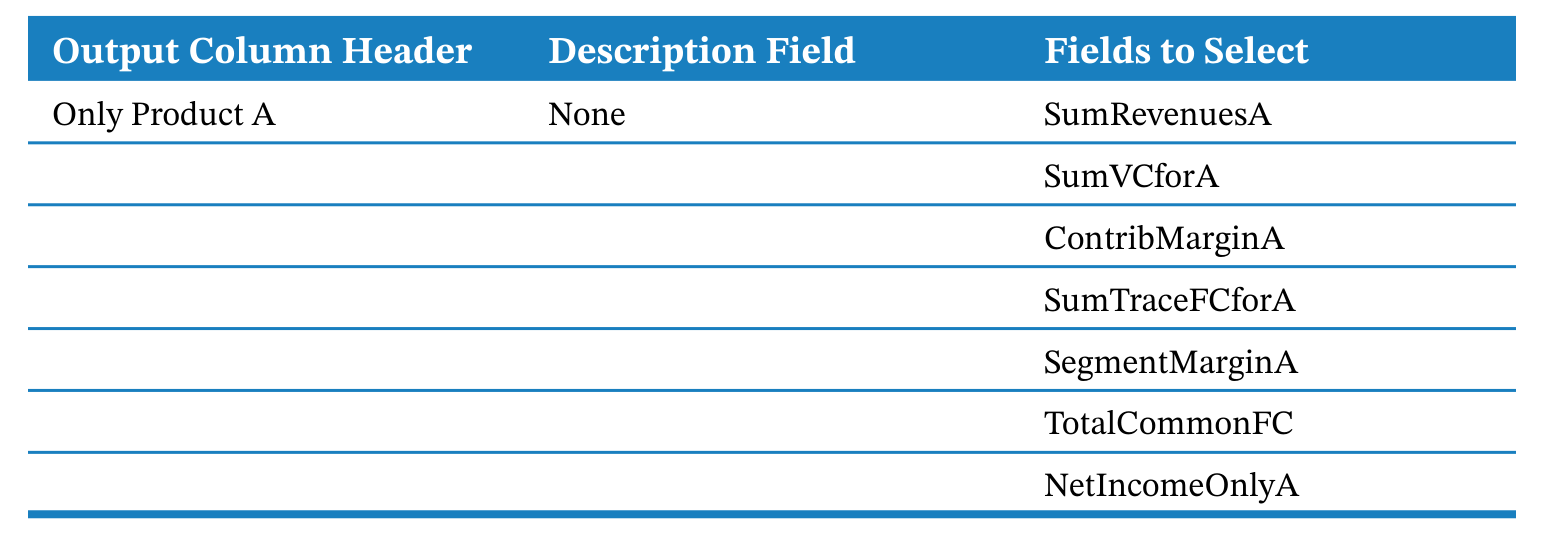
\includegraphics[width=0.95\textwidth,height=0.75\textheight,keepaspectratio]{../textbookForPractice/Figures/Ch_10/ILLUSTRATION 10.35B.png}
    \end{figure}
\end{frame}

\begin{frame}{Kế toán Thuế}
\begin{itemize}
    \item RPA tự động điền tờ khai và đối chiếu quy định pháp luật thay đổi liên tục.
    \item Phân tích rủi ro hồ sơ bị thanh tra thuế để doanh nghiệp có phương án giải trình sớm.
\end{itemize}
\end{frame}

\begin{frame}{ILLUSTRATION 10.36}

    \begin{figure}[h]
        \centering
        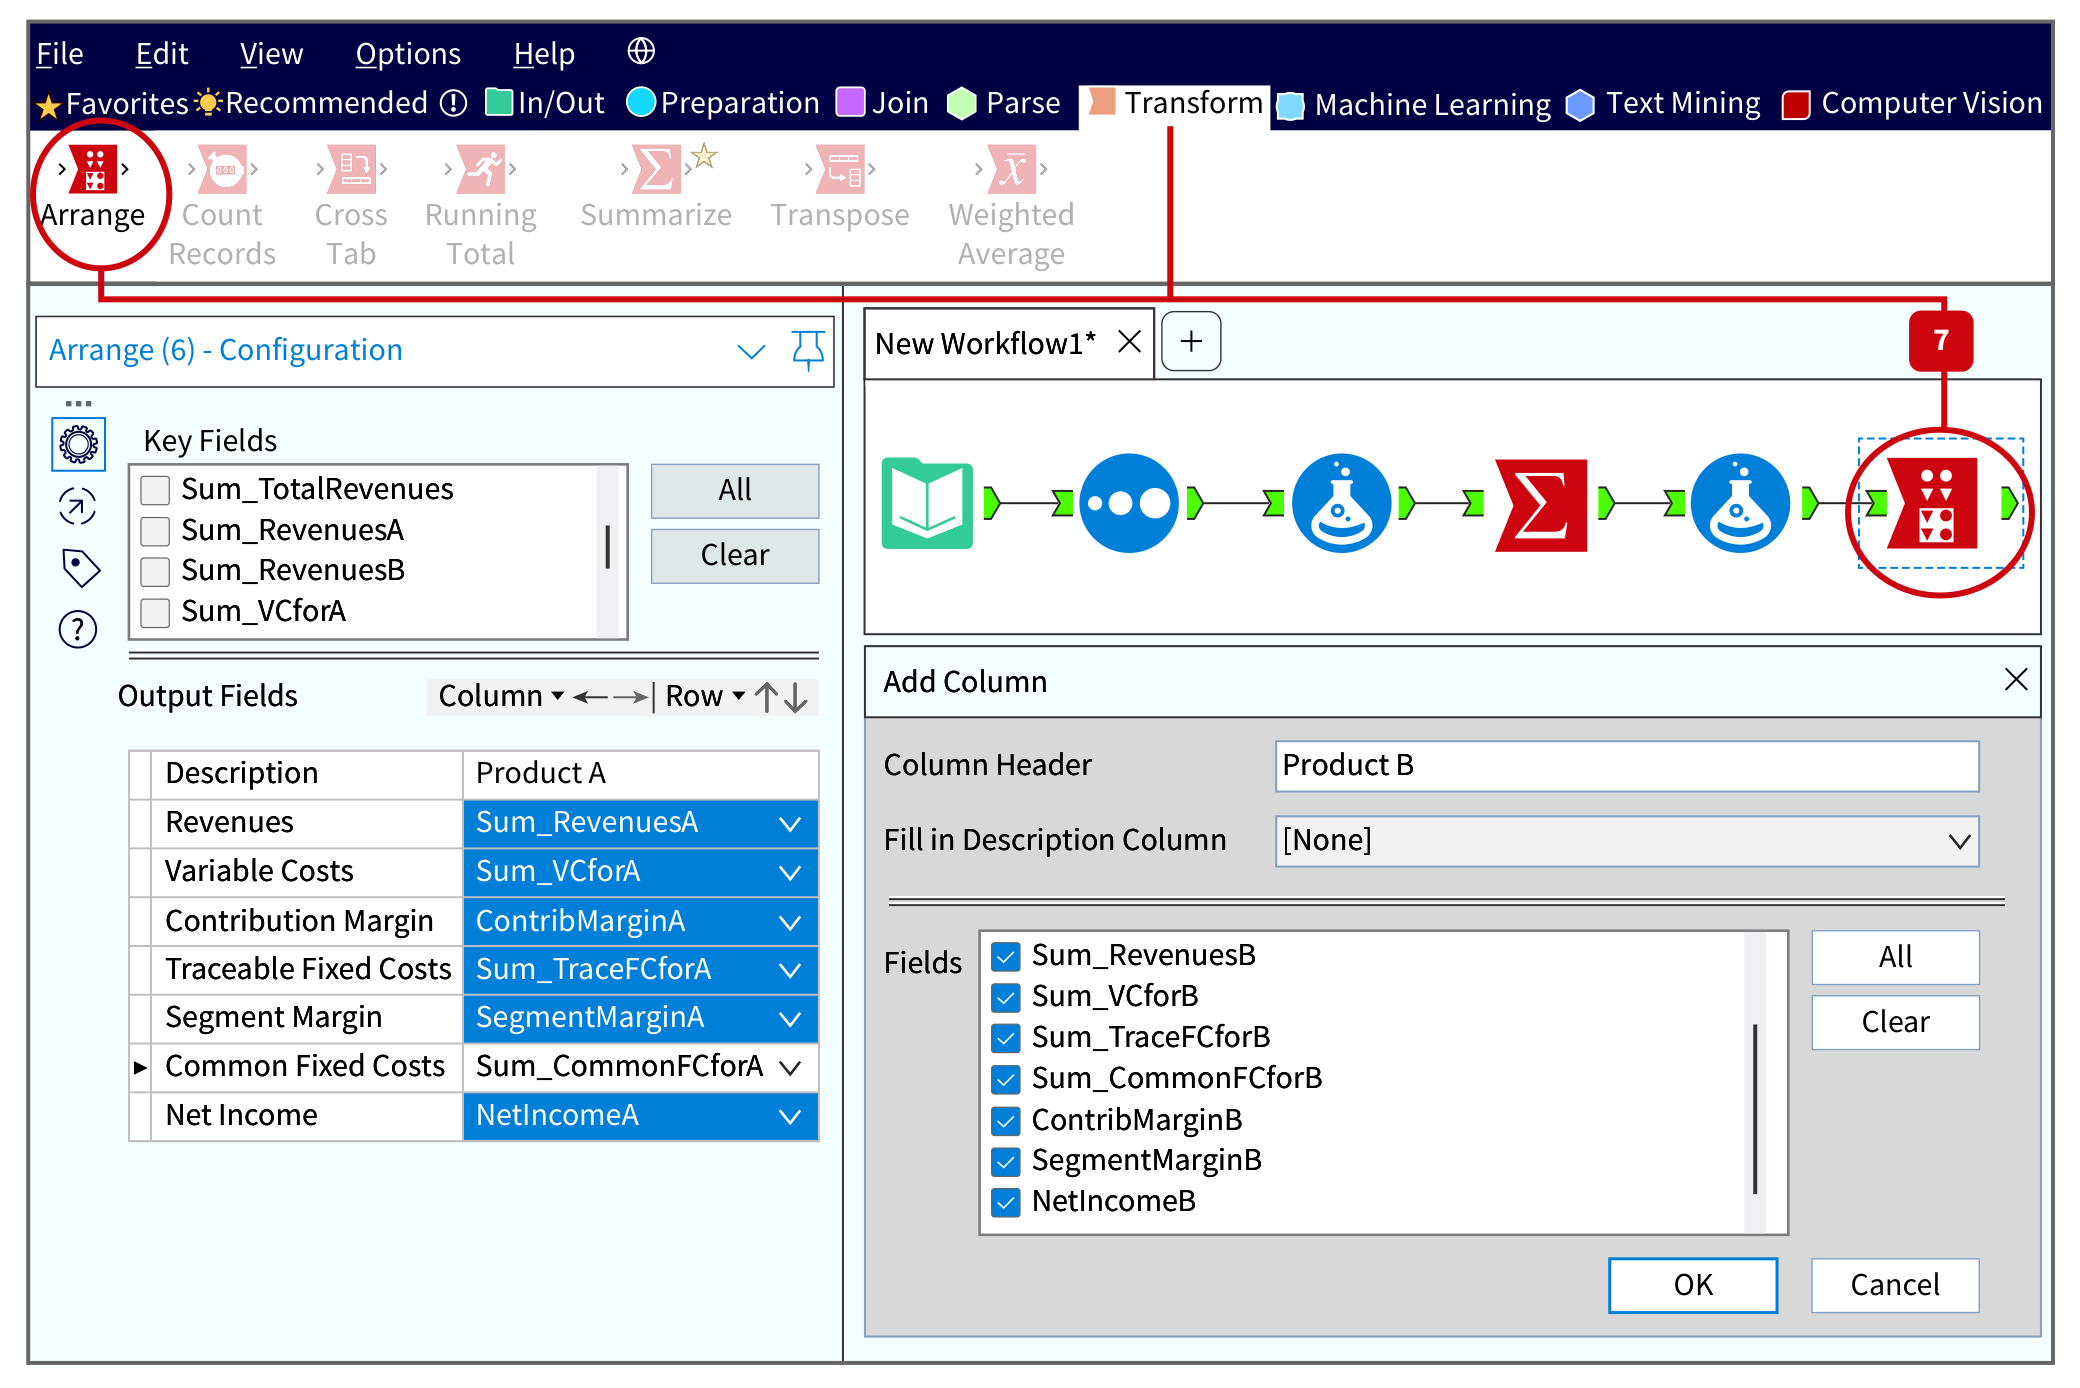
\includegraphics[width=0.95\textwidth,height=0.75\textheight,keepaspectratio]{../textbookForPractice/Figures/Ch_10/ILLUSTRATION 10.36.png}
    \end{figure}
\end{frame}

\begin{frame}{Tổng Kết Chương 10}
\begin{itemize}
    \item Nghề kế toán không biến mất, mà sẽ chuyển dịch lên cấp độ cao hơn.
    \item Công việc chân tay, lặp lại sẽ do RPA và AI đảm nhiệm.
    \item Kế toán viên cần trở thành những \textbf{Data Analyst} và \textbf{Strategic Advisor} thực thụ.
\end{itemize}
\end{frame}

\begin{frame}{ILLUSTRATION 10.37}

    \begin{figure}[h]
        \centering
        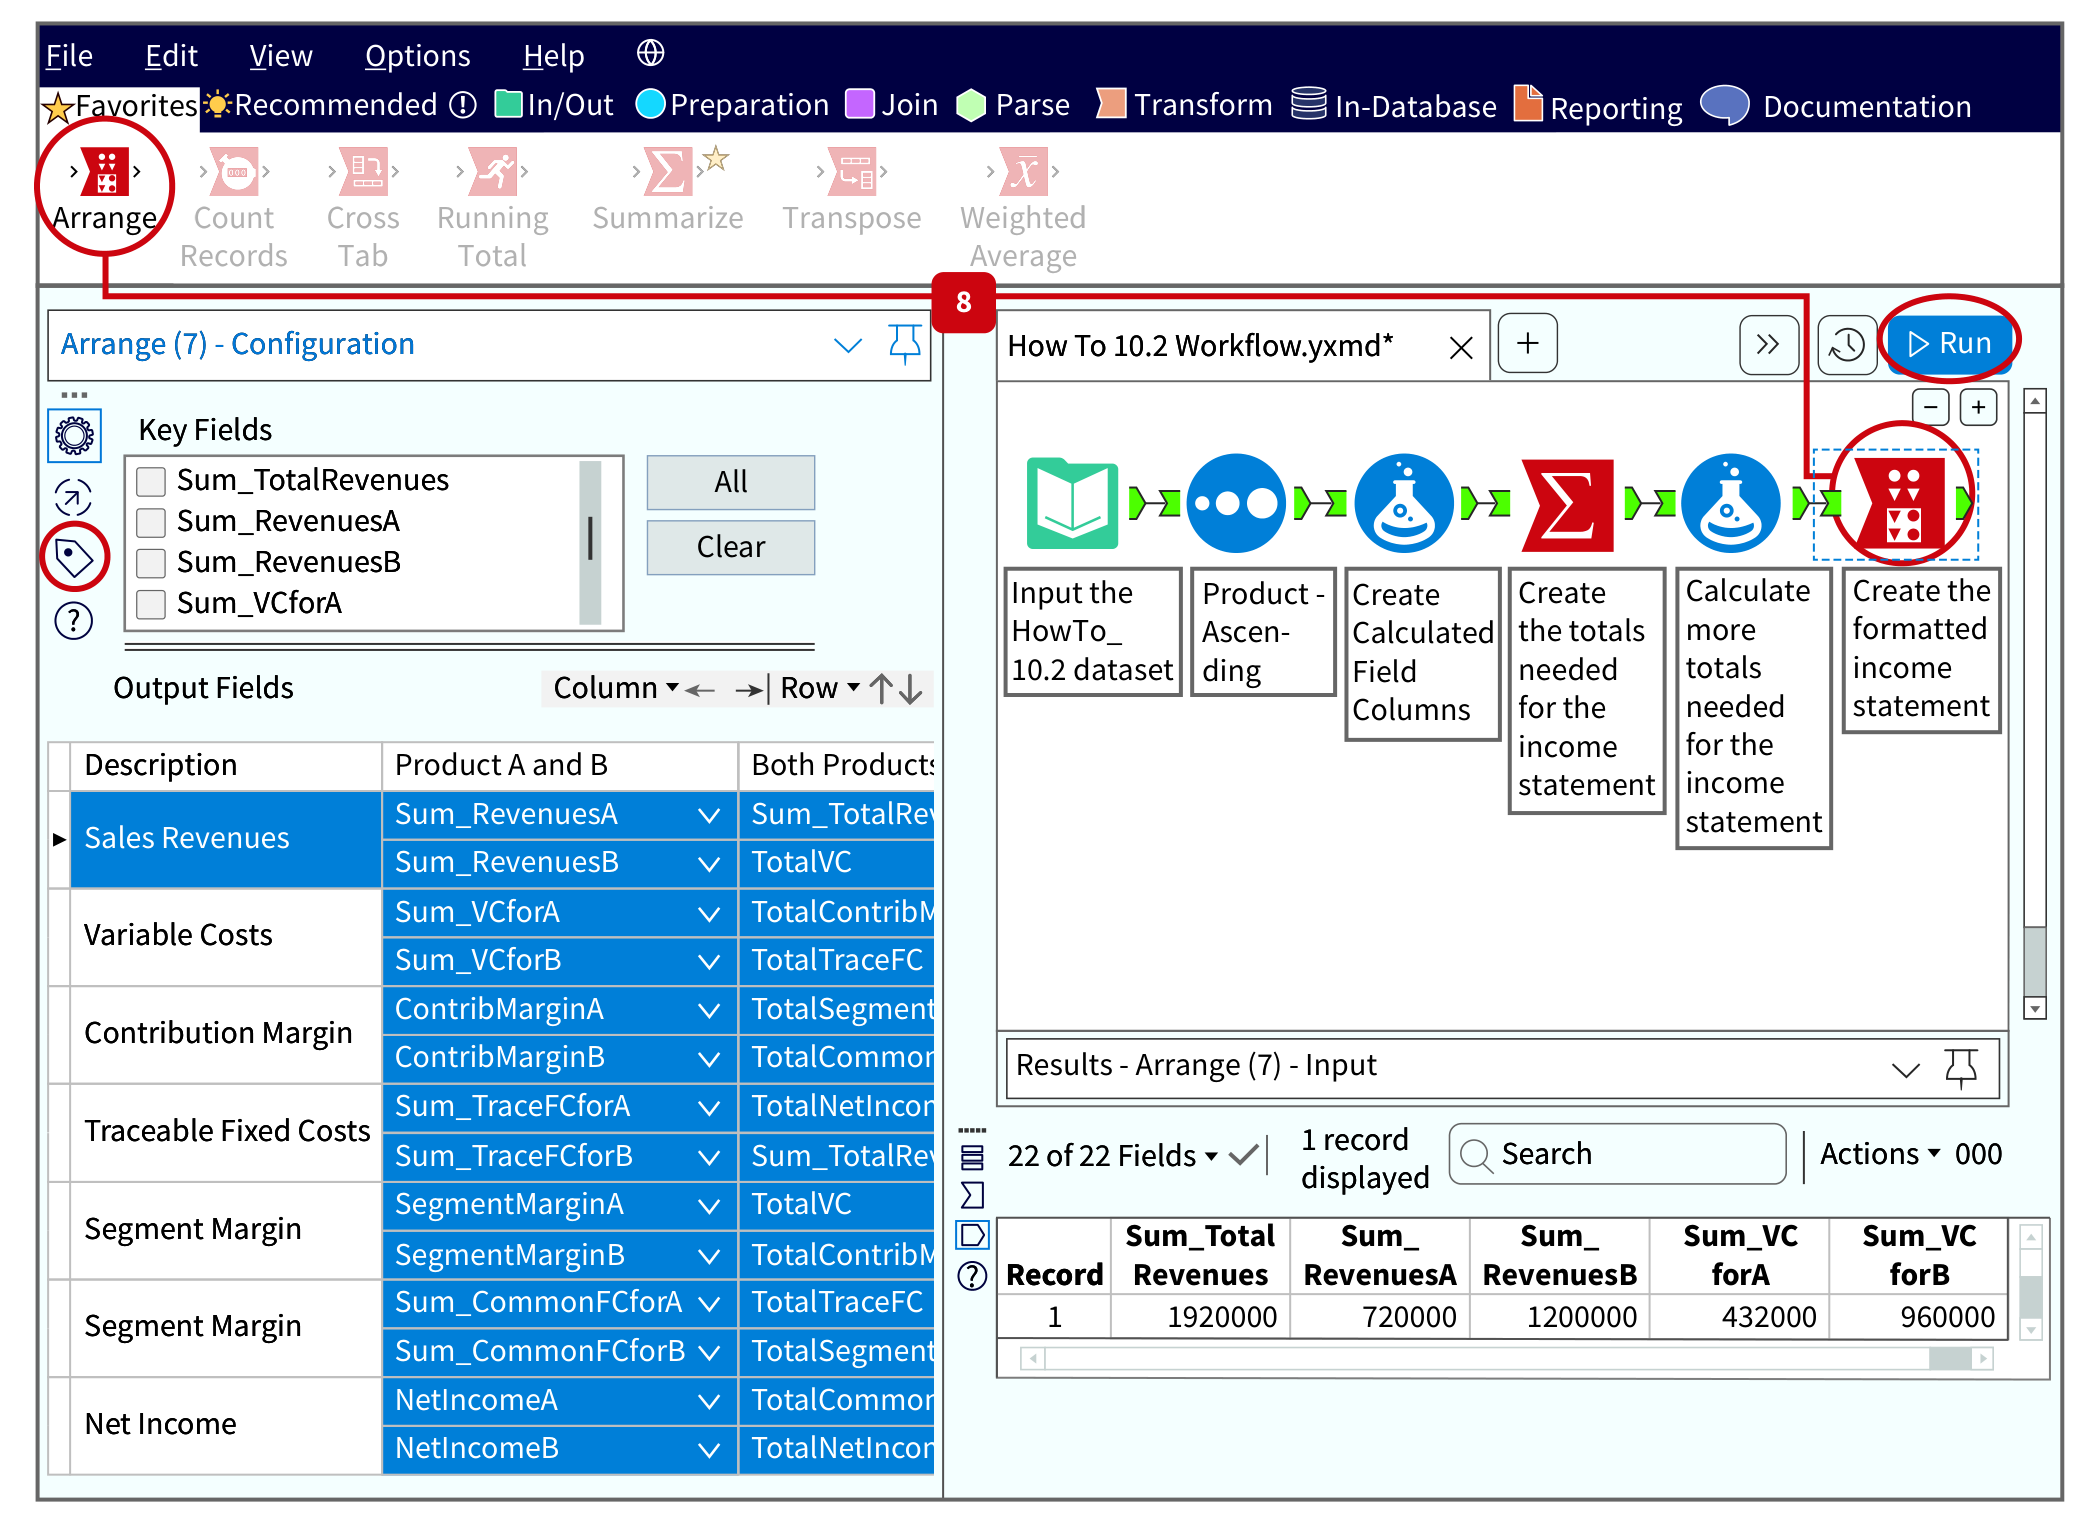
\includegraphics[width=0.95\textwidth,height=0.75\textheight,keepaspectratio]{../textbookForPractice/Figures/Ch_10/ILLUSTRATION 10.37.png}
    \end{figure}
\end{frame}

\begin{frame}{Apply It 10.1}

    \begin{figure}[h]
        \centering
        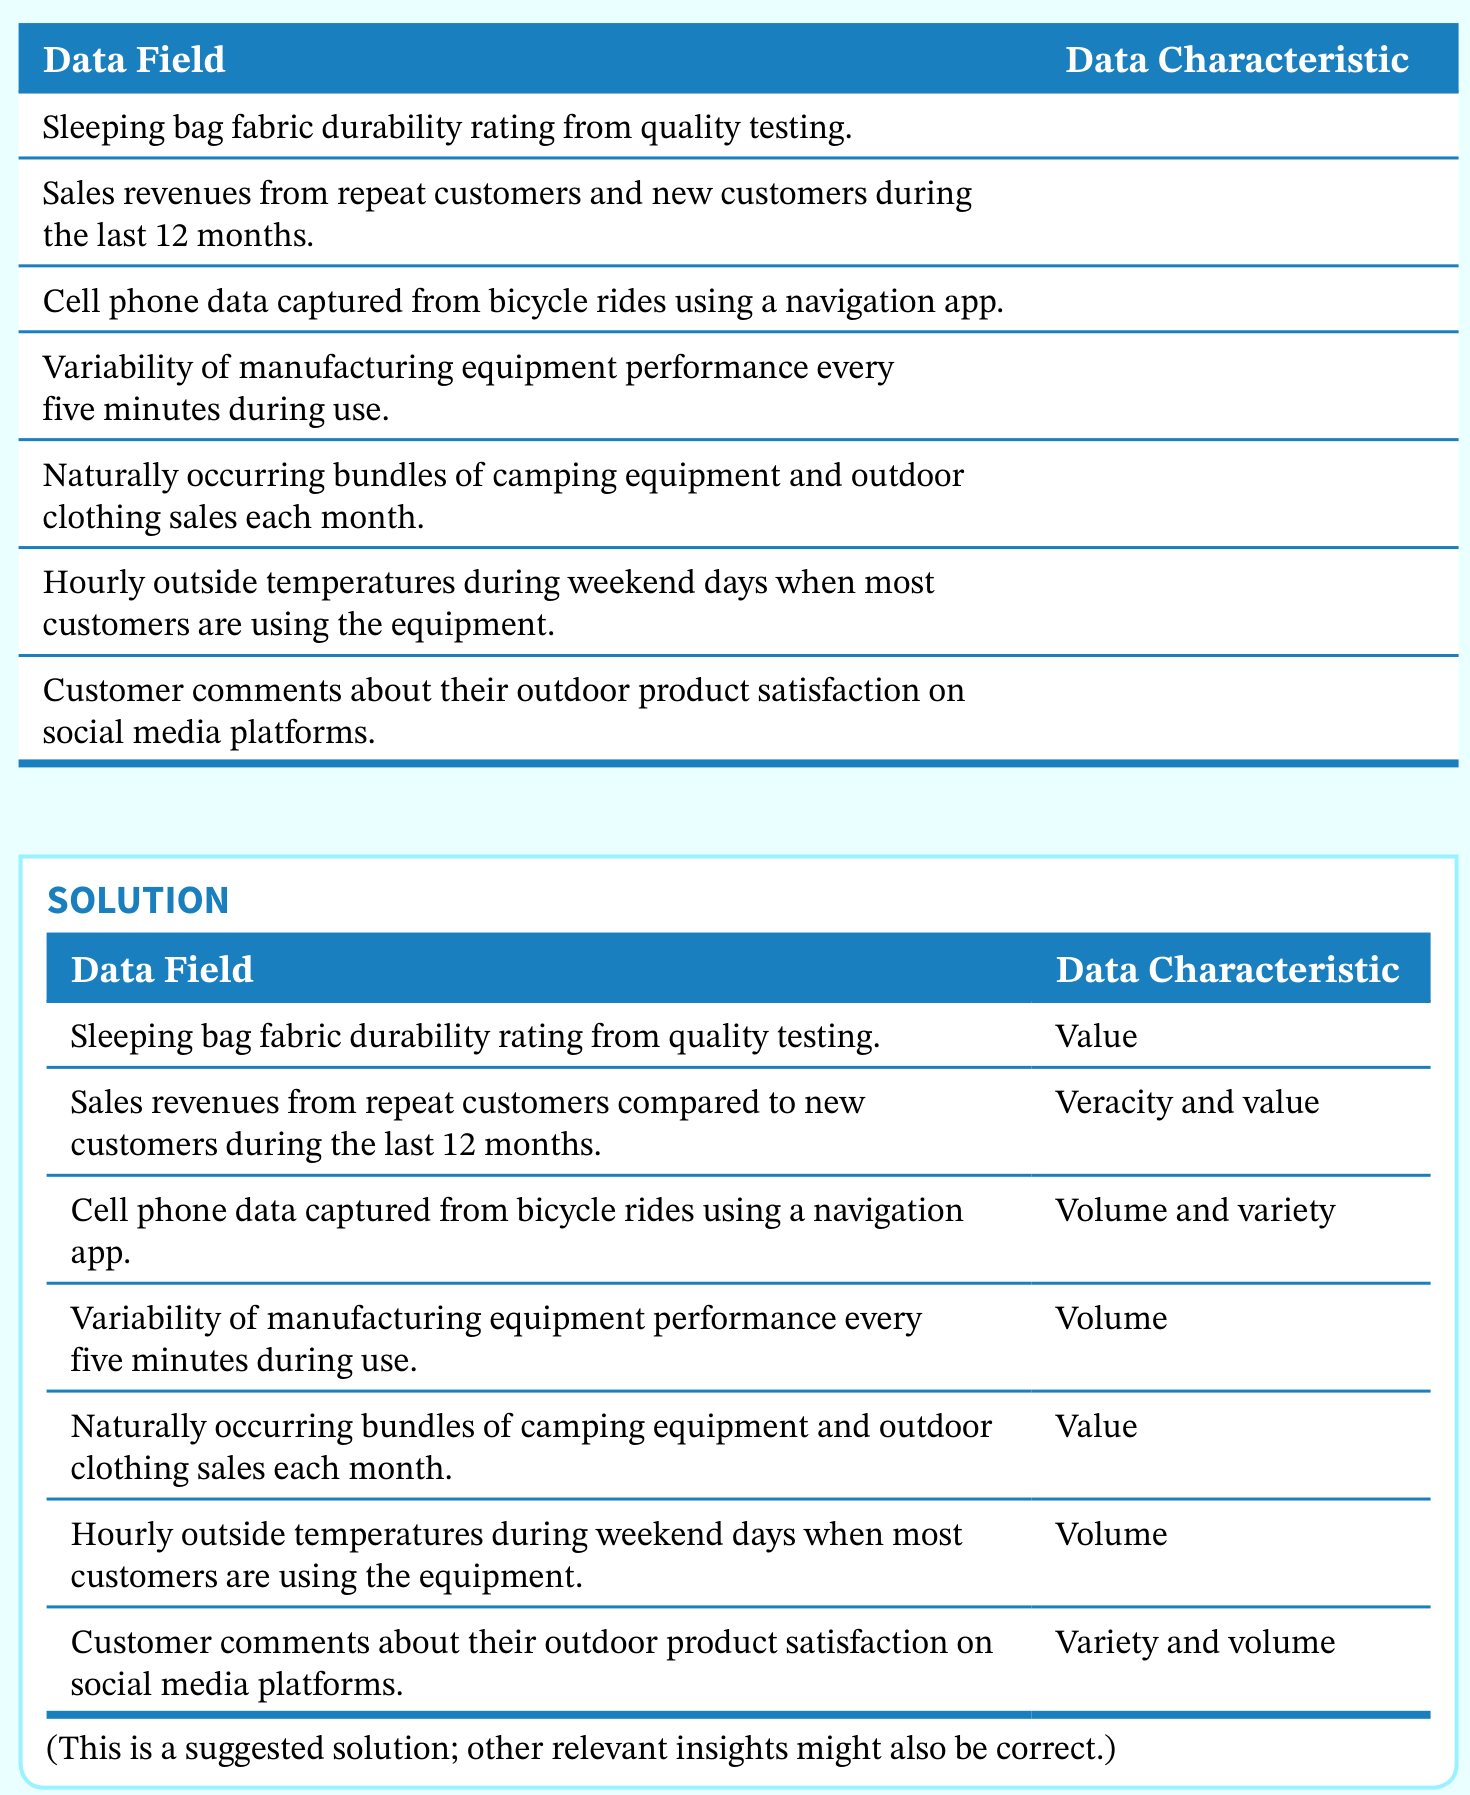
\includegraphics[width=0.95\textwidth,height=0.75\textheight,keepaspectratio]{../textbookForPractice/Figures/Ch_10/Apply It 10.1.png}
    \end{figure}
\end{frame}

\begin{frame}{Apply It 10.2}

    \begin{figure}[h]
        \centering
        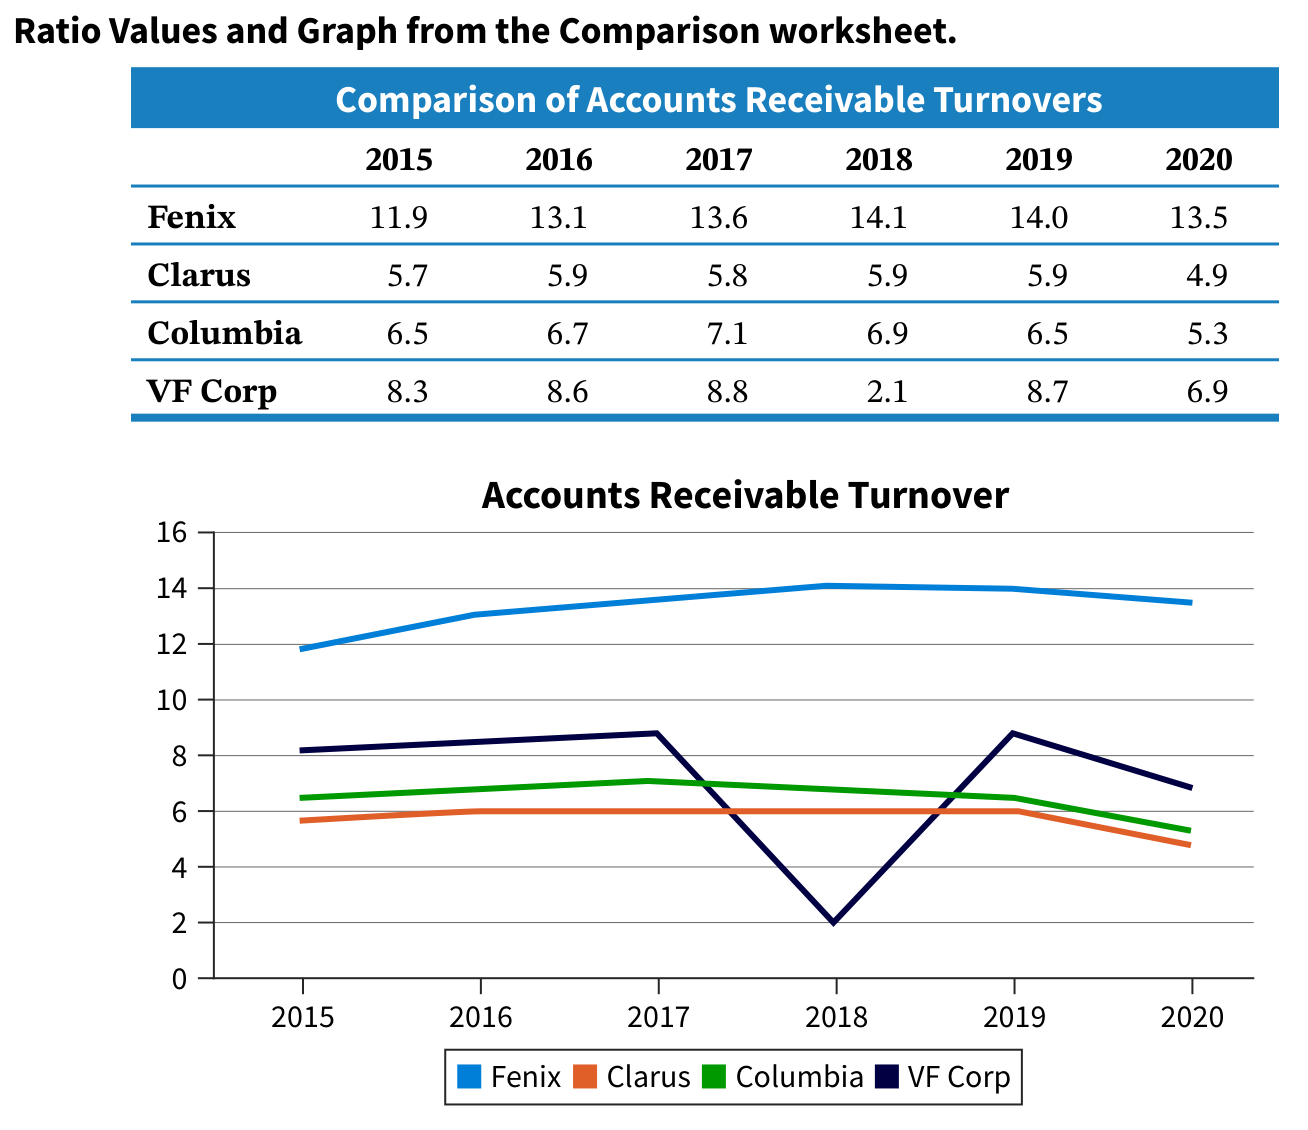
\includegraphics[width=0.95\textwidth,height=0.75\textheight,keepaspectratio]{../textbookForPractice/Figures/Ch_10/Apply It 10.2.png}
    \end{figure}
\end{frame}

\begin{frame}{HowTo 10.2}

    \begin{figure}[h]
        \centering
        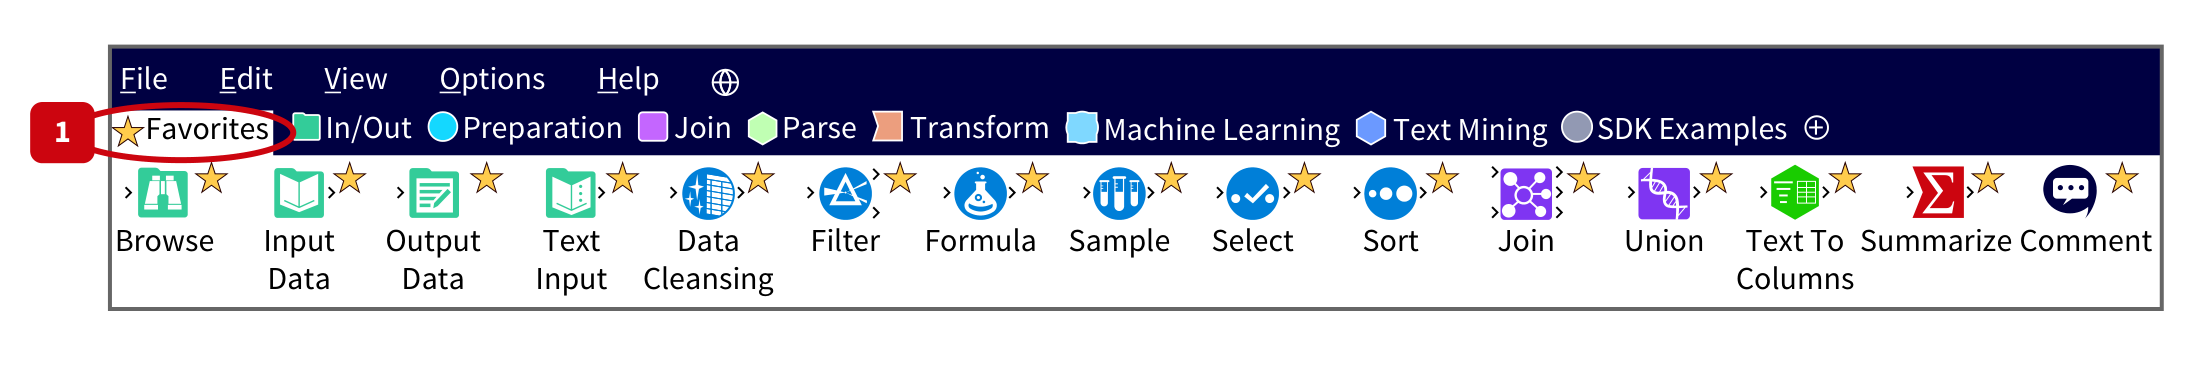
\includegraphics[width=0.95\textwidth,height=0.75\textheight,keepaspectratio]{../textbookForPractice/Figures/Ch_10/HowTo 10.2.png}
    \end{figure}
\end{frame}

\begin{frame}{Adventure Sports 10.13}

    \begin{figure}[h]
        \centering
        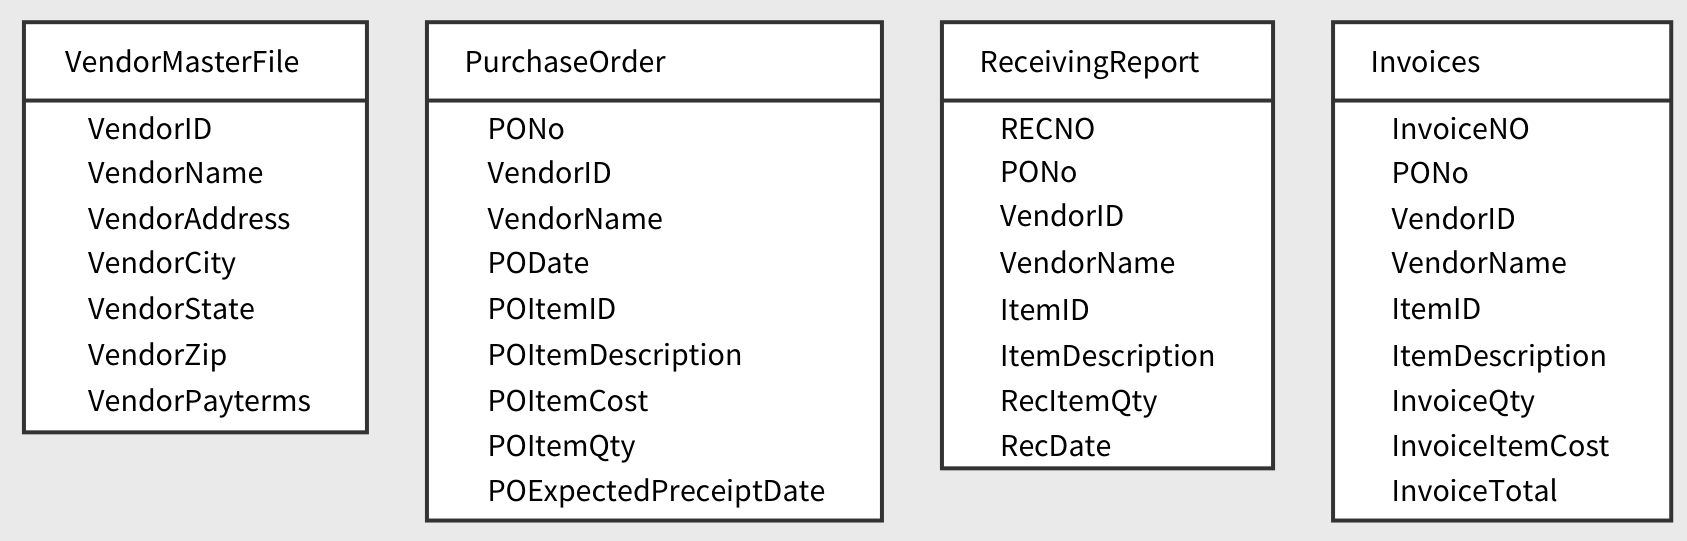
\includegraphics[width=0.95\textwidth,height=0.75\textheight,keepaspectratio]{../textbookForPractice/Figures/Ch_10/Adventure Sports 10.13.png}
    \end{figure}
\end{frame}

\begin{frame}{Bài tập Ngắn (Brief Exercises)}
\begin{center}
            \Huge \textbf{Phần Bài tập Ngắn} \\
            \vspace{0.5cm}
            \Large Brief Exercises (BE)
        \end{center}
\end{frame}

\begin{frame}{BE 10.5}

    \begin{figure}[h]
        \centering
        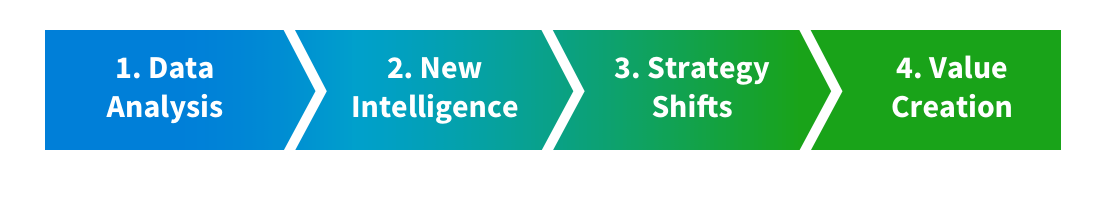
\includegraphics[width=0.95\textwidth,height=0.75\textheight,keepaspectratio]{../textbookForPractice/Figures/Ch_10/BE 10.5.png}
    \end{figure}
\end{frame}

\begin{frame}{Bài tập (Exercises)}
\begin{center}
            \Huge \textbf{Phần Bài tập} \\
            \vspace{0.5cm}
            \Large Exercises (EX)
        \end{center}
\end{frame}

\begin{frame}{EX 10.3 \& EX 10.12}
    \begin{columns}
        \begin{column}{0.5\textwidth}
            \begin{figure}[h]
                \centering
                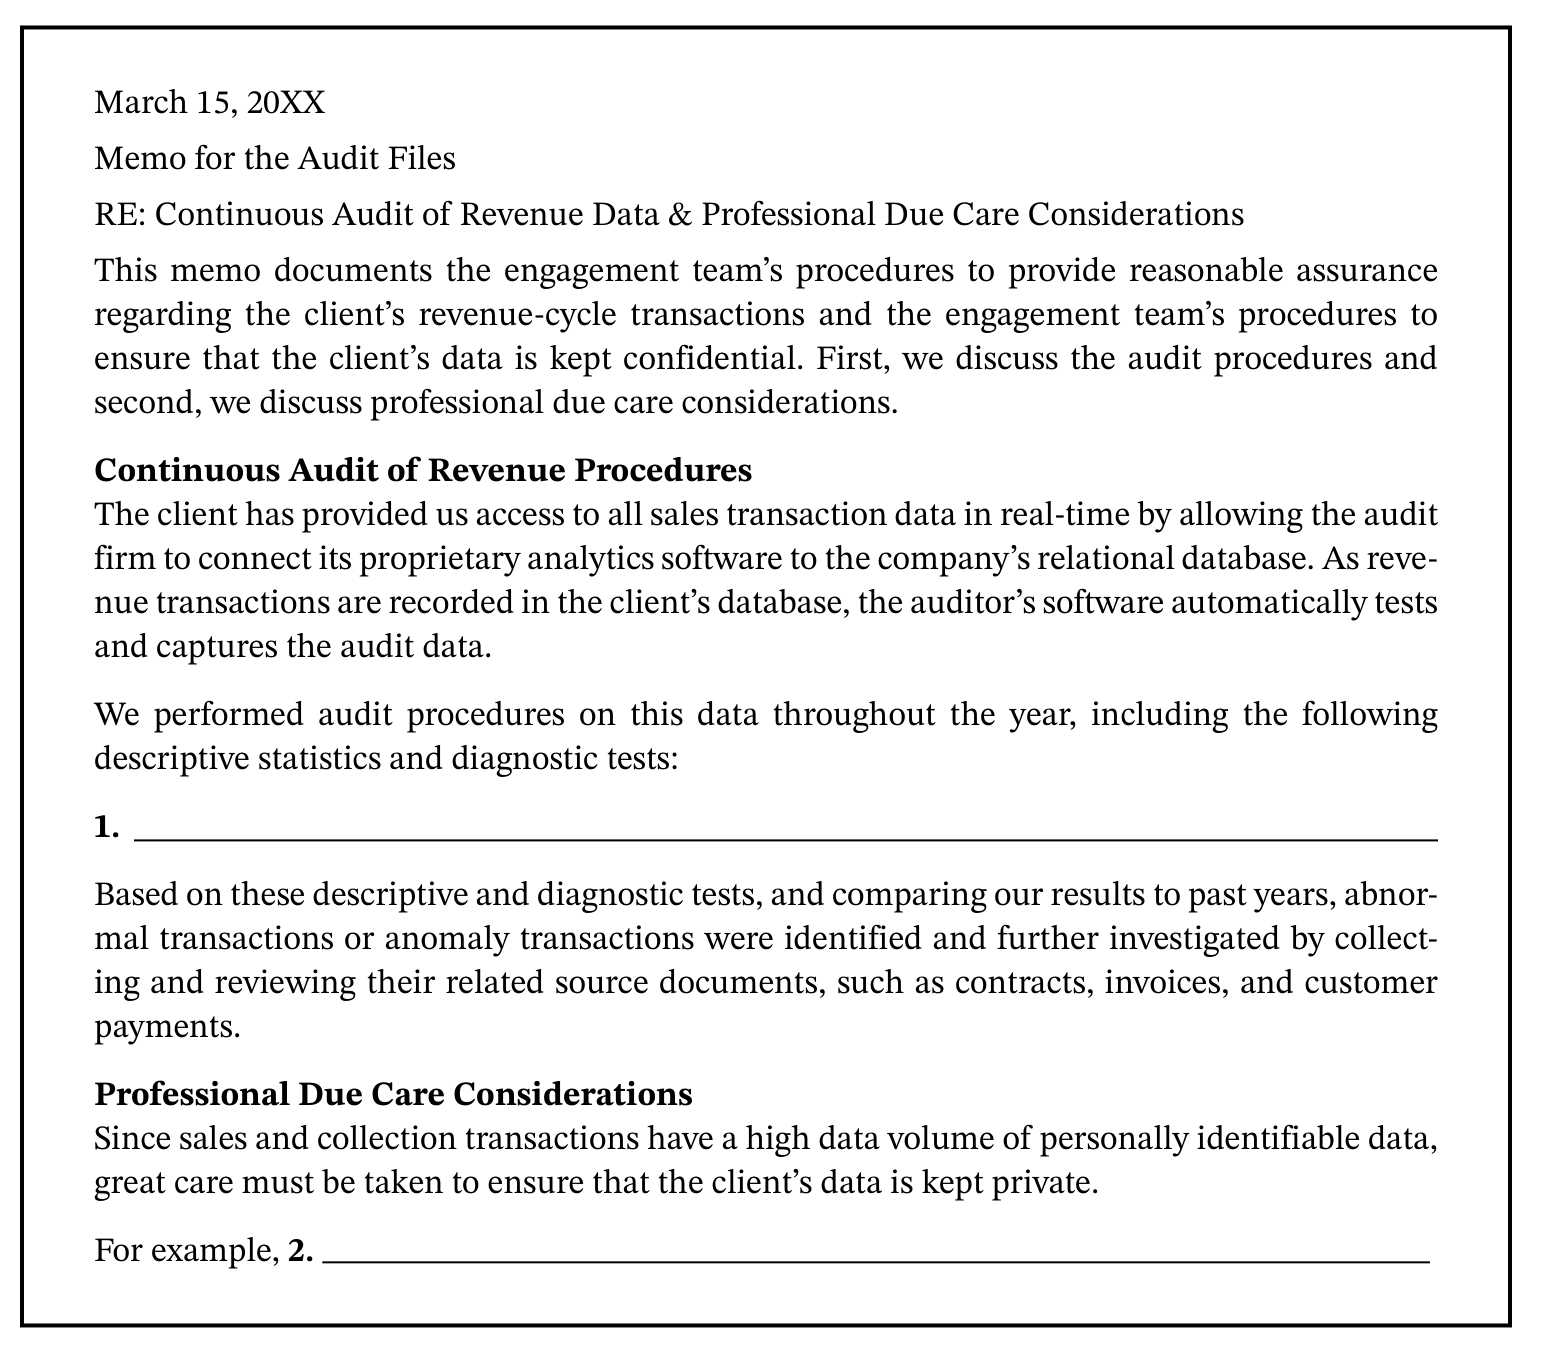
\includegraphics[width=\textwidth,height=0.7\textheight,keepaspectratio]{../textbookForPractice/Figures/Ch_10/EX 10.3.png}
            \end{figure}
        \end{column}
        \begin{column}{0.5\textwidth}
            \begin{figure}[h]
                \centering
                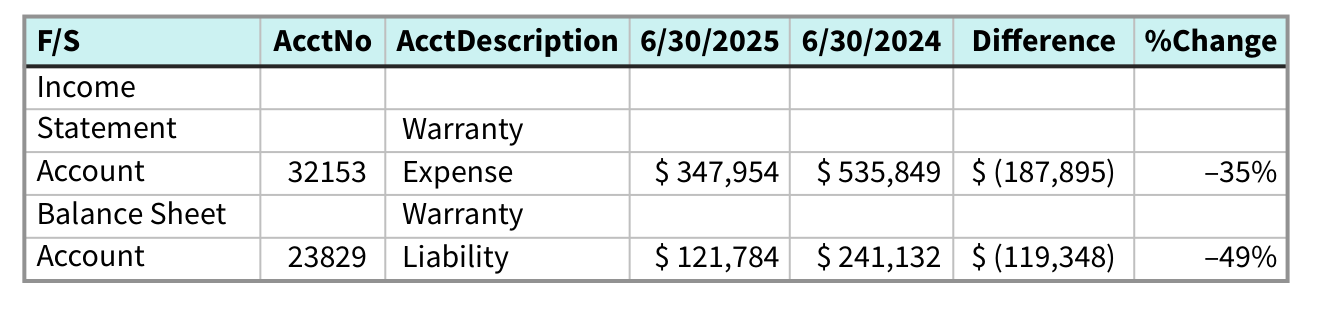
\includegraphics[width=\textwidth,height=0.7\textheight,keepaspectratio]{../textbookForPractice/Figures/Ch_10/EX 10.12.png}
            \end{figure}
        \end{column}
    \end{columns}
\end{frame}

\begin{frame}{Kết thúc}
    \begin{center}
        \Huge \textbf{Hỏi \& Đáp} \\
        \vspace{1cm}
        \Large Cảm ơn các bạn đã lắng nghe!
    \end{center}
\end{frame}

\end{document}
